% !TEX TS-program = XeLaTeX
% use the following command:
% all document files must be coded in UTF-8
\documentclass[portuguese]{textolivre}
% build HTML with: make4ht -e build.lua -c textolivre.cfg -x -u article "fn-in,svg,pic-align"

\journalname{Texto Livre}
\thevolume{14}
%\thenumber{1} % old template
\theyear{2024}
\receiveddate{\DTMdisplaydate{2024}{5}{18}{-1}} % YYYY MM DD
\accepteddate{\DTMdisplaydate{2024}{7}{16}{-1}}
\publisheddate{\today}
\corrauthor{Leonel Figueiredo de Alencar}
\articledoi{10.1590/1983-3652.2024.52653}
%\articleid{NNNN} % if the article ID is not the last 5 numbers of its DOI, provide it using \articleid{} commmand 
% list of available sesscions in the journal: articles, dossier, reports, essays, reviews, interviews, editorial
\articlesessionname{articles}
\runningauthor{Alencar} 
%\editorname{Leonardo Araújo} % old template
\sectioneditorname{Daniervelin Pereira}
\layouteditorname{Leonel Figueiredo de Alencar}

\title{Aspectos da construção de um corpus sintaticamente anotado do nheengatu no modelo Dependências Universais}
\othertitle{Aspects of the construction of a Universal Dependencies treebank for Nheengatu}
% if there is a third language title, add here:
%\othertitle{Artikelvorlage zur Einreichung beim Texto Livre Journal}

\author[1]{Leonel Figueiredo de Alencar~\orcid{0000-0001-8148-6994}\thanks{Email: \href{mailto:leonel.de.alencar@ufc.br}{leonel.de.alencar@ufc.br}}}
\affil[1]{Universidade Federal do Ceará, Centro de Humanidades, Fortaleza, CE, Brasil.}


\addbibresource{article.bib}
% use biber instead of bibtex
% $ biber article

% if you use multirows in a table, include the multirow package
\usepackage{multirow}
\usepackage{caption}
%\captionsetup[table]{name=Quadro}


% CUSTOM EPIGRAPH - BEGIN 
%%% https://tex.stackexchange.com/questions/193178/specific-epigraph-style
\usepackage{epigraph}
\renewcommand\textflush{flushright}
\makeatletter
\newlength\epitextskip
\pretocmd{\@epitext}{\em}{}{}
\apptocmd{\@epitext}{\em}{}{}
\patchcmd{\epigraph}{\@epitext{#1}\\}{\@epitext{#1}\\[\epitextskip]}{}{}
\makeatother
\setlength\epigraphrule{0pt}
\setlength\epitextskip{0.5ex}
\setlength\epigraphwidth{.7\textwidth}
% CUSTOM EPIGRAPH - END


% add line numbers for submission
%\usepackage{lineno}
%\linenumbers

% my packages
\usepackage{dirtytalk}
\usepackage{ccicons}
% my abbreviations
\newcommand{\wt}[2]{\textit{#1} `#2'}
\newcommand{\ud}{Universal Dependencies}
\newcommand{\udc}{coleção UD}
\newcommand{\tbc}{UD\_Nheengatu-CompLin}
\newcommand{\mw}{Muiratiwa}
\newcommand{\conll}{CoNLL-U}
\newcommand{\cdc}{a coleção UD}
\newcommand{\tbs}{\textit{treebanks}}
\newcommand{\tb}{\textit{treebank}}
\newcommand{\vquatro}{\textcite{de-alencar-2024-universal-k}}
\newcommand{\pvquatro}{\parencite{de-alencar-2024-universal-k}}
\newcommand{\vtres}{\textcite{alencar2023-yauti}}
\newcommand{\vum}{\textcite{alencar2021}}
\newcommand{\pvtres}{\parencite{alencar2023-yauti}}
\newcommand{\pvum}{\parencite{alencar2021}}
%\renewcommand{\sep}{;\ }

\begin{document}
\maketitle

\begin{polyabstract}
\begin{abstract}
O alheamento das tecnologias da linguagem natural constitui fator adicional de enfraquecimento de línguas minoritárias relativamente às línguas majoritárias com as quais convivem. Sobretudo os falantes mais jovens, elos da transmissão linguística, tendem a migrar para a língua favorecida com esses recursos. O nheengatu é uma língua indígena brasileira em perigo de extinção, com índice de suporte digital de apenas 0,07 na escala \textit{Digital Language Support} (DLS), significativamente inferior à pontuação de 0,97 do português, para o qual tem perdido continuamente falantes. O \textit{treebank} do nheengatu da coleção Dependências Universais visa a contribuir para redução dessa deficiência, alimentando o treinamento de um \textit{parser} neural. O \textit{treebank} estreou com 196 sentenças e 2.146 palavras na versão de 15/11/2023 dessa coleção. Este artigo trata da versão mais recente do \textit{treebank}, que, composto de amostras de sentenças extraídas de vinte publicações de diferentes fases históricas do nheengatu, perfazendo 1.470 sentenças e 15.036 palavras, constitui o maior de língua ameríndia da versão de 15/05/2024 da coleção Dependências Universais. A utilização de um analisador automático acelerou o crescimento do \textit{corpus}. Anotadores humanos, porém, revisaram cada anotação automática, assegurando um índice de validação de 100\% do \textit{treebank} e concorrendo para a classificação de duas estrelas, a mais alta conferida a \textit{treebanks} de línguas ameríndias da coleção Dependências Universais. A expansão e revisão do \textit{corpus} continuará, visando a abarcar todos os textos em domínio público e alcançar acurácia de \textit{parsing} do estado da arte.

\keywords{Linguística computacional \sep processamento de linguagem natural \sep tupinologia \sep corpus sintaticamente anotado}

\end{abstract}

\begin{english}
\begin{abstract}
The alienation of natural language technologies adds up to the weakening of minority languages coexisting with majority languages. Especially younger speakers, who function as links in language transmission, tend to migrate to the language favored by these resources. Nheengatu, an endangered Brazilian indigenous language, has a digital support score of just 0.07 on the Digital Language Support (DLS) scale. This is significantly lower than the 0.97 score for Portuguese, to which Nheengatu has been continually losing speakers. The Nheengatu treebank of the Universal Dependencies collection aims to reduce this deficit by feeding the training of a neural parser. Initially released on 11/15/2023 with 196 sentences and 2,146 words, the latest version, as of 05/15/2024, comprises 1,470 sentences and 15,036 words from twenty publications spanning different historical phases of Nheengatu. This makes it the largest treebank for an Amerindian language in the collection. The use of an automatic analyzer facilitated the rapid expansion of the corpus, while human annotators reviewed each annotation to ensure a 100\% validation rate, achieving a two-star rating, the highest for Amerindian language treebanks in the Universal Dependencies collection. The ongoing expansion and revision aim to include all public domain texts and achieve state-of-the-art parsing results.

\keywords{Computational linguistics \sep natural language processing \sep tupinology \sep treebank}

\end{abstract}
\end{english}
% if there is another abstract, insert it here using the same scheme
\end{polyabstract}

\section{Introdução}\label{sec:intro}

É fato conhecido do mundo biológico que espécies medram em ambientes propícios e definham em condições desfavoráveis. Não é diferente no campo das línguas naturais, \say{organismos vivos que, como outro vivente qualquer, nascem, crescem e se desenvolvem para culminar numa florescência [...] [exuberante] ou estiolar e morrer} \parencite[p. 63]{stradelli1929}. A história tem dado testemunho do desaparecimento de diversas línguas \parencite{Rodrigues-500-anos}. Se uma língua morre sem deixar descendentes\footnote{Sobre esse termo, ver nota \ref{footnote:descendente}.} e se, concomitantemente, não tiver sido documentada, perde-se para sempre uma peça do quebra-cabeças da linguagem ou mesmo da cognição humana \parencite{rodrigues1986linguas,storto2019}.

Num país de extrema diversidade linguística como o Brasil, a glototanásia tem vitimado diversas línguas indígenas \parencite{rodrigues1986linguas,Rodrigues-500-anos}. Das cerca de 150 línguas indígenas ainda sobreviventes no país \parencite{storto2019}, um número expressivo está ameaçado de extinção \parencite{eberhard-simons-fennig2023}. Nesse grupo se insere o nheengatu, também conhecido como tupi moderno ou Língua Geral Amazônica (LGA) \parencite{rodrigues1996,freire2011,rodrigues-cabral-2011,moore2014}. Até meados do século XIX a língua mais falada da região norte \parencite{navarro2016}, não obstante os estimados 6000 falantes no Brasil e 8000 na Colômbia, o nheengatu ocupa nesses dois países, segundo \textcite{eberhard-simons-fennig2023}, respectivamente, os níveis 6b e 7 da Escala Graduada Expandida de Interrupção Intergeracional (EGIDS, abreviatura de \textit{Expanded Graded Intergenerational Disruption Scale}). Os níveis 6b e 7 significam que, embora a geração reprodutiva ainda use o idioma, \say{a transmissão intergeracional está em vias de ser interrompida} \parencite{eberhard-simons-fennig2023}. Na Venezuela, o nheengatu ocupa o nível 8b da escala, indicando a sua quase extinção. O nível 10 da EGIDS é atribuído a línguas extintas, como, por exemplo, ao próprio tupinambá, do qual o nheengatu é descendente.\footnote{\label{footnote:descendente}\textcite{cruz2011} vale-se do modelo de árvore genealógica para classificar as línguas da família tupi-guarani. No diagrama que propõe, cada nó representa uma língua ou grupo (\say{ramo}) de línguas, conectado a um ou mais nós, de tal modo que se podem estabelecer as diferentes relações de parentesco entre as línguas ou grupos. Por exemplo, o tupinambá constitui o nó ``mãe'' do nheengatu. Em linguística histórica e comparativa, a árvore genealógica e toda a terminologia associada, como \textit{língua ancestral}, \textit{línguas filhas}, \textit{línguas parentes}, \textit{família linguística} 	\textit{etc.}, constituem  metáforas, as quais não devem ser tomadas ao pé da letra \parencite{AikhenvaldDixon2001}. Como ressalta \textcite{Faraco2022}, não é a língua que muda, mas os falantes.}

Conforme a EGIDS, a chave para a vitalidade de uma língua não é tanto o número absoluto de falantes como a transmissão natural de pais para filhos. Com apenas 780 falantes, o jamamadi, por exemplo, classifica-se no nível 5 dessa escala \parencite{eberhard-simons-fennig2023}.

Um dos fatores para a sobrevivência de uma língua nos dias de hoje é a sua presença no mundo digital. As novas gerações, exatamente aquelas responsáveis pela cadeia de transmissão de uma língua, são os usuários mais frequentes das tecnologias digitais, de cujas vidas fazem parte numa proporção dificilmente imaginada na época dos seus pais ou avós. Tradução automática, texto para voz, voz para texto e assistentes virtuais, entre outras ferramentas, representam a culminância de mais de um século de pesquisas em inteligência artificial, processamento de linguagem natural (PLN) e linguística computacional, compondo o ecossistema que determina a vitalidade dos idiomas que delas se beneficiam ou o definhamento daqueles ignorados por esse desenvolvimento científico e tecnológico.

O PLN e suas áreas afins, linguística computacional e linguística de \textit{corpus}, desenvolveram-se muito nos últimos 20 anos no Brasil, focando quase exclusivamente língua portuguesa. Paralelamente, constatamos um crescente interesse da comunidade científica internacional pela construção de recursos para o tratamento computacional de línguas minoritárias, indígenas ou em perigo de extinção. Por exemplo, \textcite{ainu-2013nlp} relatam sobre o desenvolvimento de ferramentas para processamento automático do ainu, língua nativa do norte do Japão quase extinta. Esses esforços, no entanto, praticamente ignoraram a enorme diversidade de línguas indígenas da América do Sul, representada por cerca de 456 línguas, até muito recentemente, como salientam \textcite{Gerardi2021}, que propõem uma base de dados lexical da família tupi, segundo eles, especialmente sub-representada, não obstante constituir a maior do continente. Nesse contexto, uma iniciativa digna de nota foi a criação de um \tb~para shipibo-konibo \parencite{vasquez-etal-2018-toward-k}, aparentemente o primeiro recurso desse tipo para uma língua ameríndia no modelo Dependências Universais (doravante UD) \parencite{nivre-etal-2016-universal-k,de-marneffe-etal-2021-universal-k}. 

Felizmente, o ostracismo tecnológico a que se relegaram as línguas indígenas brasileiras começa a reverter-se. \textcite{Galves2017} e \textcite{sandalo2023anotando} discutem a elaboração de um esquema de anotação para um \textit{corpus} sintaticamente anotado (\tb) do cadiuéu. \textcite{rueter-etal-2021-apurina-k} relatam sobre as diferentes etapas da construção do primeiro \tb~do apurinã no modelo UD, visando à implementação de aplicações de PLN de alto nível, v.g., sistemas de resolução de perguntas (QA, do inglês \textit{question answering}), tradução automática \textit{etc.} \textcite{DAngelis-2021} tratam da tradução do sistema operacional de um fabricante de celulares para caingangue e nheengatu. \vum~descreve um tradutor automático para predicações qualificativas em nheengatu, língua para a qual \vtres~propõe uma ferramenta denominada Yauti capaz de construir árvores no formato UD. \textcite{martin-rodriguez-etal-2022-tupian-k,santos2024linguas} apresentam diversos recursos computacionais para línguas tupis, incluindo \tbs~no modelo UD para nove membros dessa família.

O presente trabalho vem somar-se a esses esforços, constituindo mais um passo para dirimir a disparidade de condições de sobrevivência do nheengatu frente ao português.\footnote{Conforme \textcite{eberhard-simons-fennig2023}, o espanhol parece pouco usado entre falantes do nheengatu. De um lado, resta, quando muito, um número ínfimo de falantes na Venezuela. De outro lado, na Colômbia, vem ocorrendo uma migração do nheengatu para a língua tucano.} Com a progressiva absorção, a partir do último quartel do século XIX, dos seus falantes à cultura de língua portuguesa, ancorada na escrita, o nheengatu, de tradição essencialmente oral, enfraqueceu-se cada vez mais, perdendo terreno adicional com a televisão e a internet, sobretudo entre os falantes mais jovens \parencite{navarro-avila-trevisan-2017}. A concorrência com a língua portuguesa tornou-se ainda mais desfavorável com a disseminação avassaladora das tecnologias de linguagem natural. \textcite{simons-etal-2022-assessing-k} enfatizam a importância do suporte digital para a sobrevivência de uma língua num mundo mediado digitalmente, fator para o qual propõem cálculo de pontuação de 0 a 1 e classificação numa escala de cinco faixas sequenciadas de forma ascendente (Figura \ref{fig:digital-support}). 

\begin{figure}[htbp]
  \centering
  \begin{minipage}{.75\textwidth}
    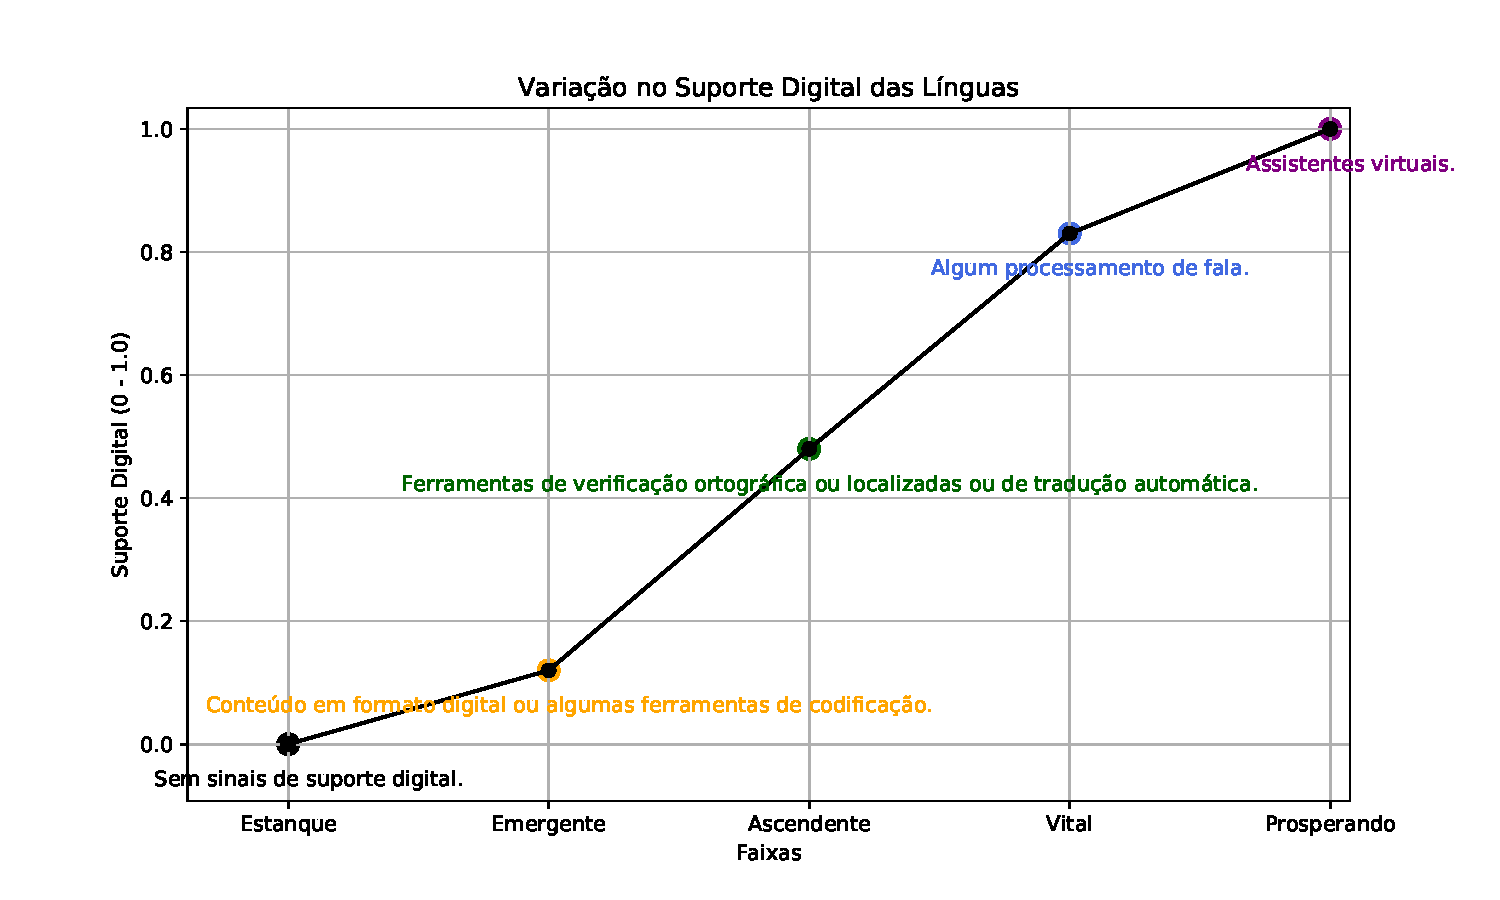
\includegraphics[width=\linewidth]{figures/DigitalSupportColors.pdf}
    \caption{Escala de Suporte Digital às Línguas (DLS, do inglês \textit{Digital Language Support}).}
    \label{fig:digital-support}
    \source{Elaboração própria a partir das especificações de \textcite{simons-etal-2022-assessing-k,eberhard-simons-fennig2023}.}
  \end{minipage}
\end{figure}
 
O nheengatu, com base nessa escala, enquadra-se na categoria de línguas com suporte digital emergente, contudo, a pontuação alcançada é de apenas 0,07 \parencite{eberhard-simons-fennig2023}, a uma gigantesca distância de línguas majoritárias como português e inglês, com pontuações de 0,97 e 1,0. 

O desenvolvimento de ferramentas robustas de PLN é uma tarefa de engenharia de software não trivial. O que para o usuário final ocorre num passe de mágica oculta nos bastidores um edifício de conhecimentos e técnicas acumulados e aperfeiçoados durante décadas. Trata-se de complexo passível de divisão numa série de componentes encadeados, de tal forma que o desempenho de um componente depende essencialmente daquele que o precede na cadeia. Um dos componentes essenciais é a análise sintática automática (\textit{syntactic parsing}), da qual depende a análise semântica e, consequentemente, a compreensão textual automática, base, por sua vez, para aplicações como sistemas de QA, tradutores automáticos, assistentes virtuais \textit{etc.} 

Este artigo trata do \tbc, aparentemente o único \tb~sintático do nheengatu.\footnote{O \tbc~com os respectivos arquivos \texttt{stats.xml} e \texttt{eval.log} e os principais \textit{scripts} utilizados para processar esses dados encontram-se neste \href{https://osf.io/t3uws/?view_only=265e1e44ff3f45e989d5f978ba7dfd80}{link}. Os três primeiros arquivos integram a versão 2.14 da \udc~ \parencite{zeman2024universal}. O repositório \url{https://github.com/CompLin/nheengatu} contém a versão mais atualizada do \tb~e das respectivas ferramentas.}  Distribuído sob a licença \href{https://creativecommons.org/licenses/by-nc-sa/4.0/}{\ccbyncsa}, expandiu-se de 196 sentenças e 2.146 palavras na versão v2.11 da \udc~para 1.470 e 15.036 na versão atual (Figura \ref{fig:evolucao-muiratiwa}). Esse tipo de recurso permite construir um analisador sintático automático (\textit{parser}) por meio de aprendizagem de máquina, utilizando, por exemplo, redes neurais \parencite{straka-etal-2016-udpipe-k}. Sua utilidade, porém, transcende o domínio da informática. A linguística de \textit{corpus} passou a constituir a partir da última década um método padrão de levantamento de dados nos mais variados domínios das ciências da linguagem, da dialetologia e sociolinguística à linguística histórica, passando pela teoria gramatical, sanando limitações de dados obtidos por introspecção \parencite{hirschmann2019korpuslinguistik}.

\begin{figure}[htbp]
  \centering
  \begin{minipage}{.9\textwidth}
    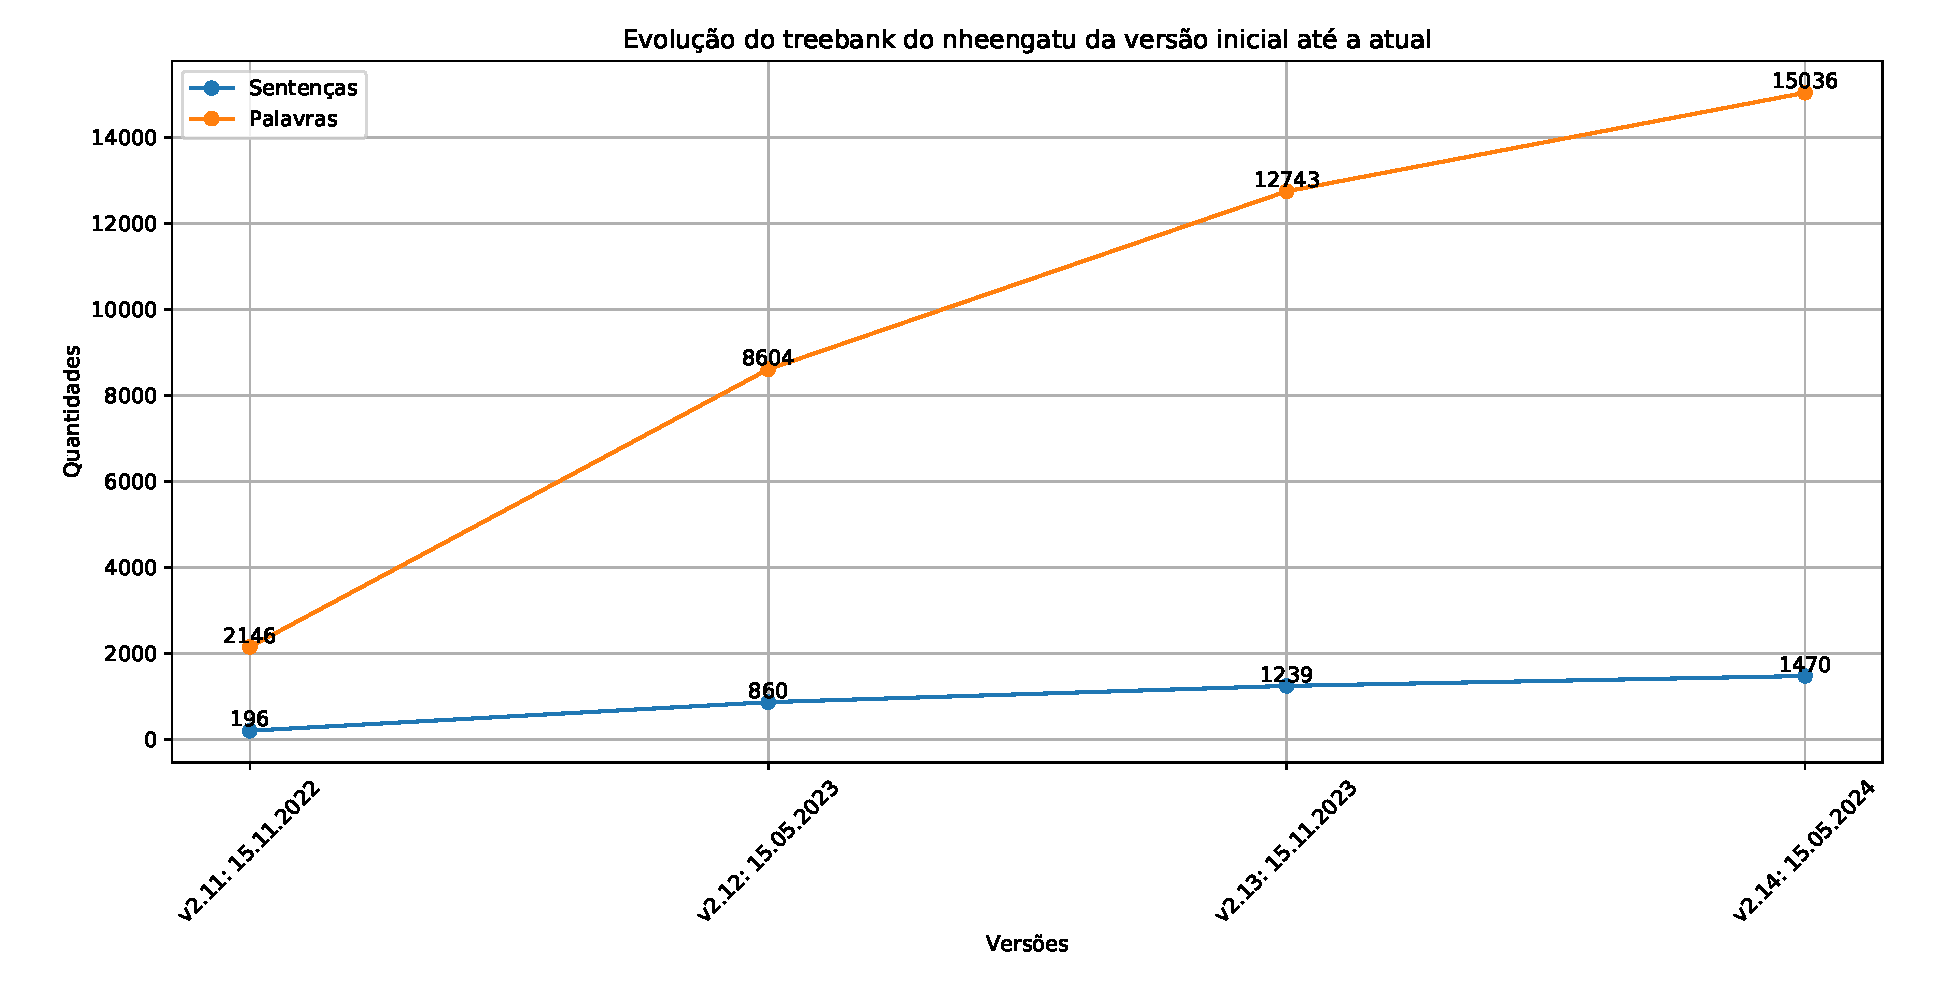
\includegraphics[width=\linewidth]{figures/NheengatuTBEvolution.pdf}
    \caption{Crescimento do \tbc.}
    \label{fig:evolucao-muiratiwa}
    \source{Elaboração própria.}
  \end{minipage}
\end{figure}

Na próxima seção, expomos o quadro teórico que fundamentou a construção do \tb. A seção seguinte trata da metodologia, focando a seleção dos textos, a normalização ortográfica e o fluxograma de anotação e revisão. A seção \ref{sec:anotacao} aborda as diferentes dimensões da anotação. A última seção apresenta as conclusões e oferece sugestões para trabalhos futuros.

\section{Aspectos do projeto UD}\label{sec:ud}

Mirando tanto investigações linguísticas quanto a interpretação semântica e aplicações de PLN, UD almeja consistência na anotação morfossintática de línguas tipologicamente as mais diversas \parencite{de-marneffe-etal-2021-universal-k}, no âmbito de um esforço coletivo no espírito do código aberto que resultou numa coleção de 283 \tbs~de 161 línguas, em contínua expansão desde 2015 (Figura \ref{fig:crescimento}).  

\begin{figure}[htbp]
  \centering
  \begin{minipage}{\textwidth}
    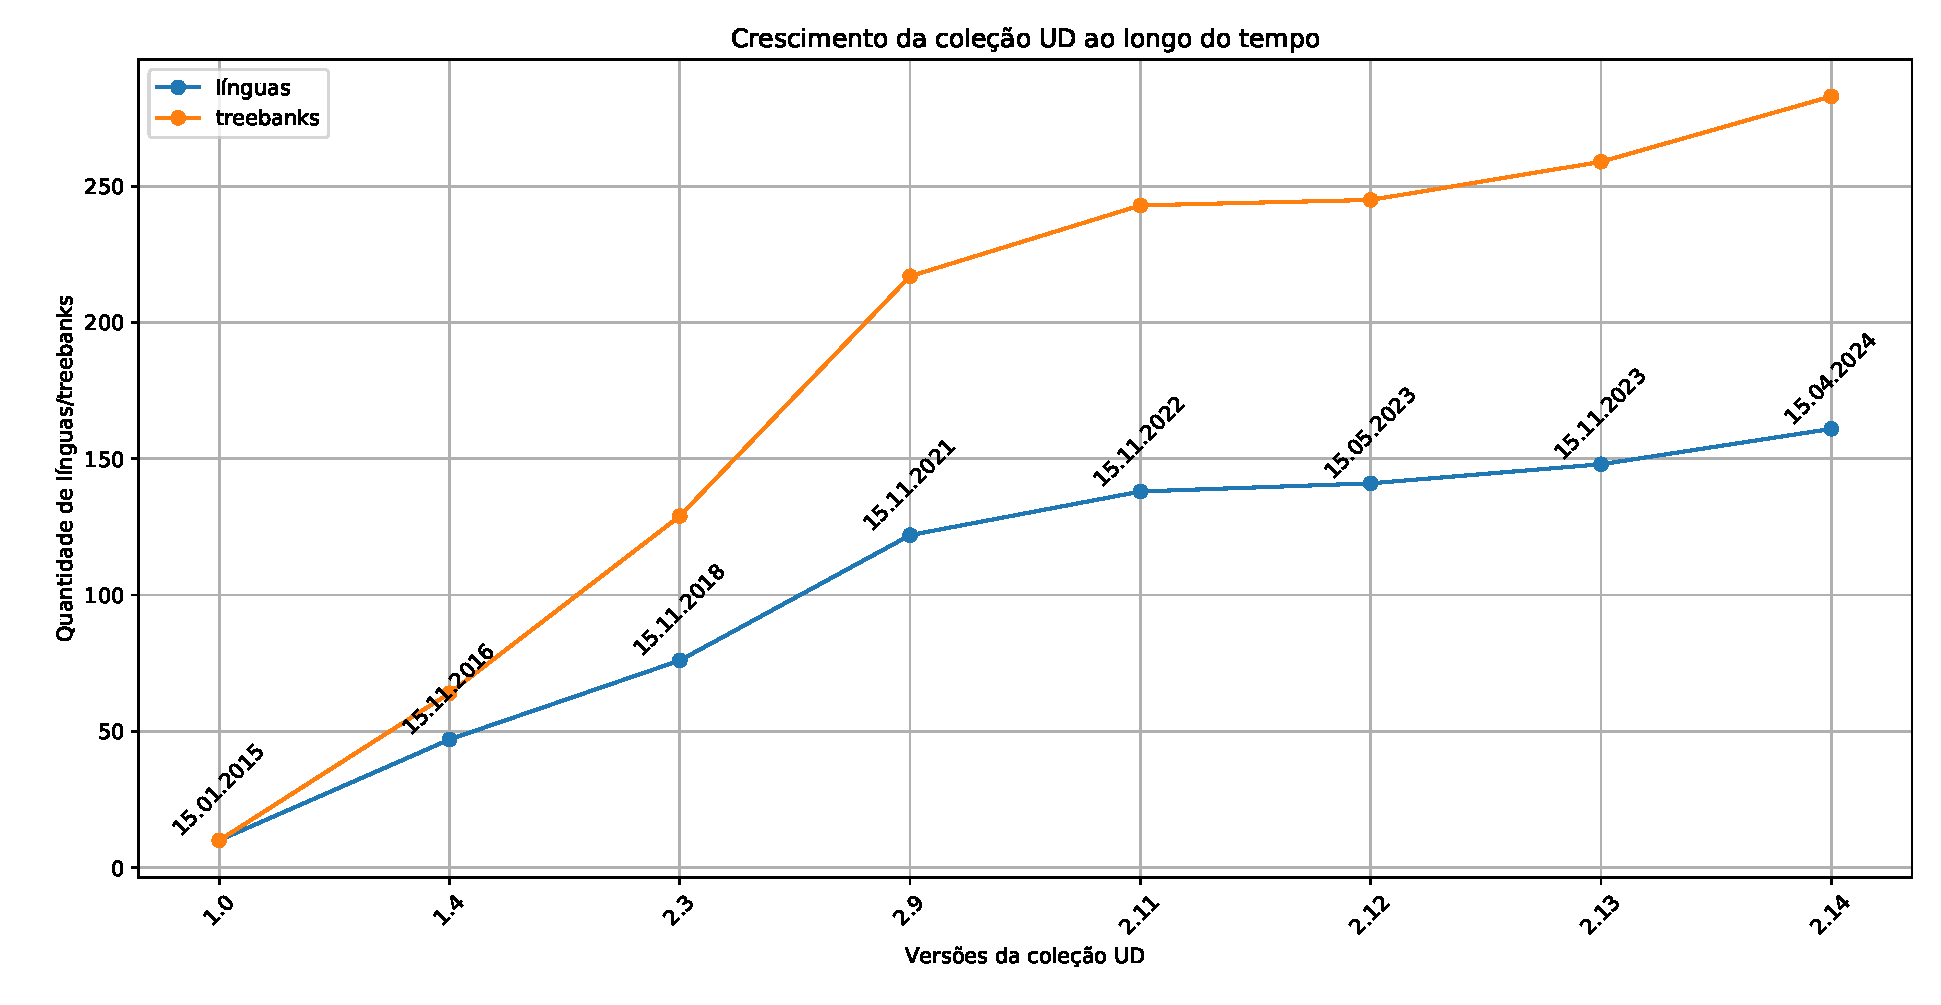
\includegraphics[width=\linewidth]{figures/CrescimentoUD.pdf}
    \caption{Crescimento da \udc~do início até a versão atual.}
    \label{fig:crescimento}
    \source{Elaboração própria com base nos dados de \textcite{Upos2024}.}
  \end{minipage}
\end{figure}

\begin{figure}[htbp]
  \centering
  \begin{minipage}{.7\textwidth}
    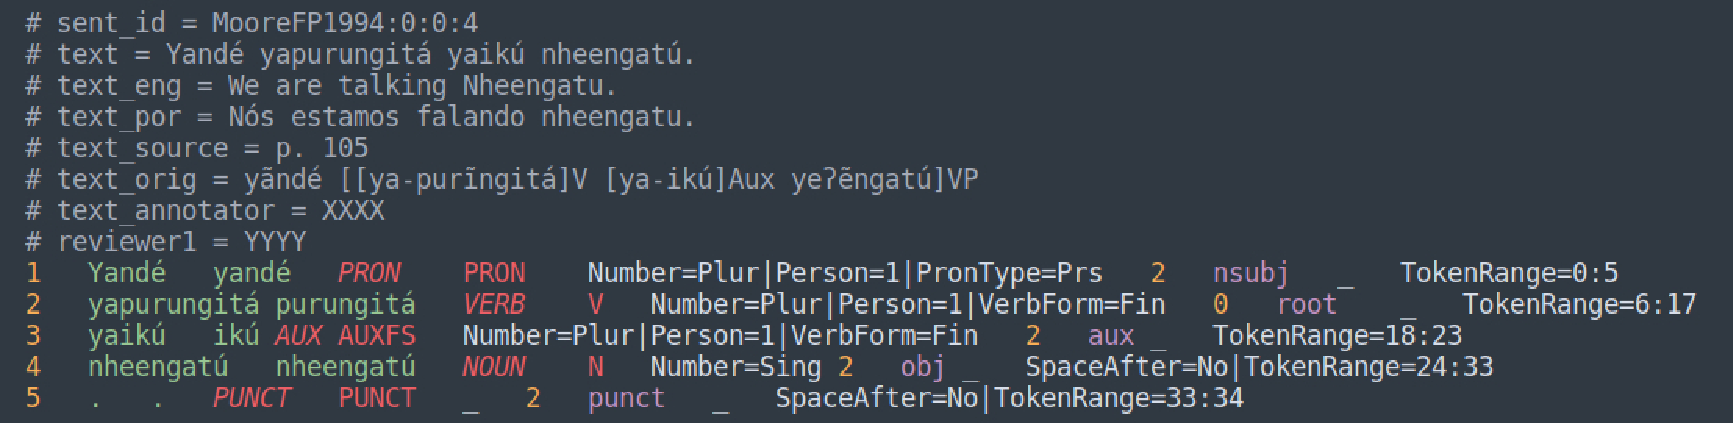
\includegraphics[width=\linewidth]{figures/moore-4-conllu.pdf}
    \caption{Análise de sentença do \tbc~no formato \conll.}
    \label{fig:conllu}
    \source{Elaboração própria.}
  \end{minipage}
\end{figure}

A Figura \ref{fig:conllu} exemplifica o formato \conll~do modelo UD. O primeiro componente consiste em uma série de metadados encabeçados por \texttt{\#}, enquanto o segundo é uma tabela de dez colunas separadas por tabulações, com uma linha para cada palavra. Essas colunas especificam, para cada palavra, as seguintes informações, nesta ordem: (i) índice de ordem (ID); (ii) forma (FORM); (iii) lema (LEMMA); (iv) etiqueta do conjunto de partes do discurso universais (UPOS) (\Cref{tab:upos}); (v) classe de palavra de um conjunto XPOS de etiquetas específicas da língua em questão; (vi) traços morfológicos (FEATS); (vii) núcleo regente (HEAD); (viii) relação de dependência (DEPREL); (ix) \say{dependências aprimoradas} (\textit{enhanced dependencies}) (DEPS) e (x) informações adicionais (MISC). Por exemplo, a forma \wt{yaikú}{estamos} porta o índice 3, uma vez que é a terceira da sentença. O lema dessa palavra é o radical \wt{ikú}{estar}. Diferentemente do verbo pleno \wt{purungitá}{conversar} da linha 2, etiquetado como \texttt{VERB} na respectiva coluna (iv), o auxiliar \wt{ikú}{estar} classifica-se como \texttt{AUX} no modelo UD. Um \tb~da coleção UD não precisa especificar todos esses campos, mas apenas (i), (iv), (vii) e (viii). A coluna (ix), que abriga as chamadas dependências aprimoradas \parencite{schuster-manning-2016-enhanced-k}, é preenchida apenas por parte dos \tbs~da coleção UD.

\begin{table}[htbp]
\caption{Etiquetas do conjunto UPOS.}
\centering
\begin{tabular}{|l|l|l|}
\hline
\textbf{Palavras de classe aberta} & \textbf{Palavras de classe fechada} & \textbf{Outras} \\ \hline
ADJ: adjetivo & ADP: adposição & PUNCT: sinal de pontuação \\ \hline
ADV: advérbio & AUX: auxiliar & SYM: símbolo \\ \hline
INTJ: interjeição & CCONJ: conjunção coordenativa & X: outra \\ \hline
NOUN: nome comum & DET: determinante &  \\ \hline
PROPN: nome próprio & NUM: numeral &  \\ \hline
VERB: verbo & PART: partícula &  \\ \hline
 & PRON: pronome &  \\ \hline
 & SCONJ: conjunção subordinativa &  \\ \hline
\end{tabular}
\label{tab:upos}
\source{Adaptado de \textcite{Upos2024}.}
\end{table}

A \Cref{tab:upos} exibe as 17 etiquetas de partes do discurso do conjunto UPOS, postuladas como universais, ou seja, capazes de classificar qualquer palavra de qualquer língua. No entanto, o conjunto de partes do discurso de uma língua particular não precisa coincidir com UPOS, podendo constituir um subconjunto \parencite{de-marneffe-etal-2021-universal-k}. O modelo UD agrupa as diferentes classes em três macrocategorias, as duas primeiras das quais abrangem a noção tradicional de palavra. A primeira macrocategoria consiste em conjuntos passíveis de contínua expansão, por exemplo, por meio de processos de formação de palavras ou empréstimos de outras línguas, enquanto a segunda macrocategoria abarca as palavras de classe fechada, que constituem conjuntos relativamente fixos, que raramente incorporam novos membros \parencite{jurafsky2009,Lehmann2013-nature}. Tipicamente, a criação de novos membros das classes fechadas ocorre pela gramaticalização de itens de classe aberta \parencite{Lehmann2013-nature}. Um exemplo do nheengatu é o substantivo \wt{pukusawa}{comprimento}, que passou a funcionar como posposição (`durante') e conjunção (`enquanto') \parencite{cruz2011,avila2021}.\footnote{Cumpre ressaltar que os critérios para definição dessas duas macrocategorias variam conforme o arcabouço teórico. \textcite[p. 27]{Lehmann2013-nature}, por exemplo, considera adposições e conjunções como \say{classes abertas em todas as línguas europeias modernas.}} 

A terceira macrocategoria consiste de sinais de pontuação, símbolos e qualquer outro tipo de material textual que não se enquadre em nenhuma das demais classes. Sinais de pontuação são tratados no modelo UD como os demais \textit{tokens} que representam palavras num sentido tradicional, ocupando, como estas, nós na árvore sintática, ligados a outros nós por relações de dependência (Figura \ref{fig:dep-tree}).\footnote{Todas as árvores dependenciais deste artigo foram geradas pelo visualizador \url{https://www.let.rug.nl/kleiweg/conllu/}.} 

Com exceção da classe de particípio, subsumida na classe dos verbos, as duas primeiras macrocategorias da \Cref{tab:upos} englobam as taxonomias óctuplas grega e latina antigas \parencite{Robins1966-ROBTDO-13} e a classificação de palavras de \textcite{macambira1999} e \textcite{rocha2011gramatica}, entre outros, que, na esteira da Nomenclatura Gramatical Brasileira (NGB), consideram substantivo, pronome, artigo, advérbio, verbo, preposição, conjunção, interjeição, adjetivo e numeral suficientes para abarcar todo o léxico do português. Na teoria UD, os artigos integram a classe dos determinantes, que abriga muitos dos itens tratados como pronomes em abordagens mais tradicionais, como indefinidos, interrogativos e demonstrativos. Dado seu viés tipológico, a teoria UD substituiu a categoria preposição pela adposição, que abrange tanto preposições quanto posposições e circumposições. Diferentemente da NGB, a classe numeral do modelo UD, seguindo modelos precedentes de anotação de \tbs~como o de \textcite{santorini1990}, se restringe aos numerais cardinais, excluindo, por exemplo, em línguas como o português, palavras como \textit{segundo} ou \textit{terceiro}, analisadas como adjetivos \parencite{duran2021manual}.\footnote{Pelo contrário, \textcite{francis1979manual} prescrevem a etiquetagem de cardinais e ordinais como \texttt{CD} e \texttt{OD}.} As outras discrepâncias do modelo UD em relação à NGB são a categoria partícula e a subdivisão de verbos, substantivos e conjunções nas classes \texttt{VERB}, \texttt{AUX}, \texttt{NOUN}, \texttt{PROPN}, \texttt{CCONJ} e \texttt{SCONJ}. 

A classificação de numerais cardinais e interjeições é controversa. \textcite{greenberg2000numeral} observa que cardinais comportam-se de forma análoga tanto a adjetivos quanto substantivos em várias línguas, com o que \textcite{evans2000word} concorda, destacando, por outro lado, a rígida estruturação formal e semântica desses elementos, característica de palavras de classe fechada. Em gramática gerativa, há autores que enxergam uma natureza lexical nos cardinais, classificando-os como substantivos ou adjetivos, enquanto outros os analisam como categoria funcional Num ou Q, que projeta um sintagma numeral (NumP) ou quantificador (QP), respectivamente \parencite{ionin2018cardinals}. \textcite{tesniere1959elements} classifica o cardinal em \wt{deux livres}{dois livros} como adjetivo de quantidade, tratando as interjeições como tipo não de palavra, mas de sentença, designando-as \wt{mots-phrases}{palavras-frase}. Analogamente, \textcite[p. 92]{cunha2017} excluem a interjeição das diferentes classificações que postulam para palavras e morfemas, dada a sua natureza de \say{vocábulo-frase} ou \say{grito com que traduzimos de modo vivo nossas emoções}\parencite[605]{cunha2017}. Pelo contrário, \textcite{ameka1992interjections} ressalta o caráter provavelmente universal das interjeições, considerando-as uma classe de palavras. \textcite[p. 120]{wilkins1992interjections} contesta a inserção das interjeições \say{no cesto de lixo dos `fenômenos paralinguísticos`}. Para ele, a interjeição constitui simultaneamente um lexema e um enunciado, relevando à investigação teórica nas mais diferentes subdisciplinas da linguística. No tratamento da interjeição, o modelo UD se soma a uma prática na construção de \textit{corpora} anotados que remonta a \textcite{francis1979manual} e, posteriormente, a \textcite{santorini1990}, em cujos esquemas de anotação essa parte do discurso figura sob a etiqueta \texttt{UH}. 

O conjunto XPOS do \tbc~constitui-se de 78 etiquetas, incorporando tanto distinções correntes na descrição do nheengatu, como a subclassificação dos pronomes pessoais em primeira e segunda classes \parencite{navarro2016,avila2021}, ou a subdivisão dos verbos em ativos (dinâmicos) e inativos (estativos) \parencite{cruz2011}, quanto distinções de granularidade mais fina que visam a capturar particularidades semânticas e/ou morfossintáticas. No \tbc, via de regra, subdivisões de uma categoria do conjunto UPOS no âmbito do conjunto XPOS são indicadas por sufixos que refletem as propriedades diagnósticas de cada subgrupo. Por exemplo, as etiquetas \texttt{AUXFS} e \texttt{AUXFR} do conjunto XPOS distinguem auxiliares flexionados pós-verbais (Figura \ref{fig:dep-tree}) e pré-verbais (Figura \ref{fig:aux-su}), respectivamente.  

\begin{figure}[htbp]
  \centering
  \begin{minipage}{.7\textwidth}
    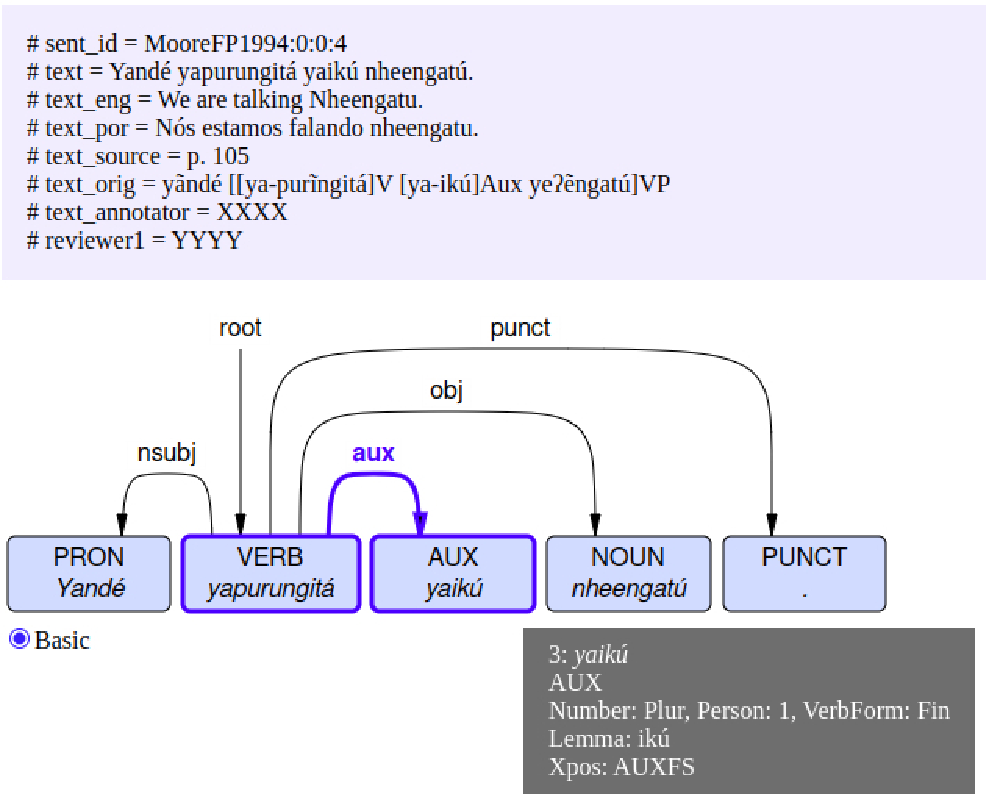
\includegraphics[width=\linewidth]{figures/moore-4.pdf}
    \caption{Representação dependencial de sentença do \tbc~destacando os traços da forma \textit{yaikú} `estamos'.}
    \label{fig:dep-tree}
    \source{Elaboração própria.}
  \end{minipage}
\end{figure}

\begin{figure}[htbp]
  \centering
  \begin{minipage}{.7\textwidth}
    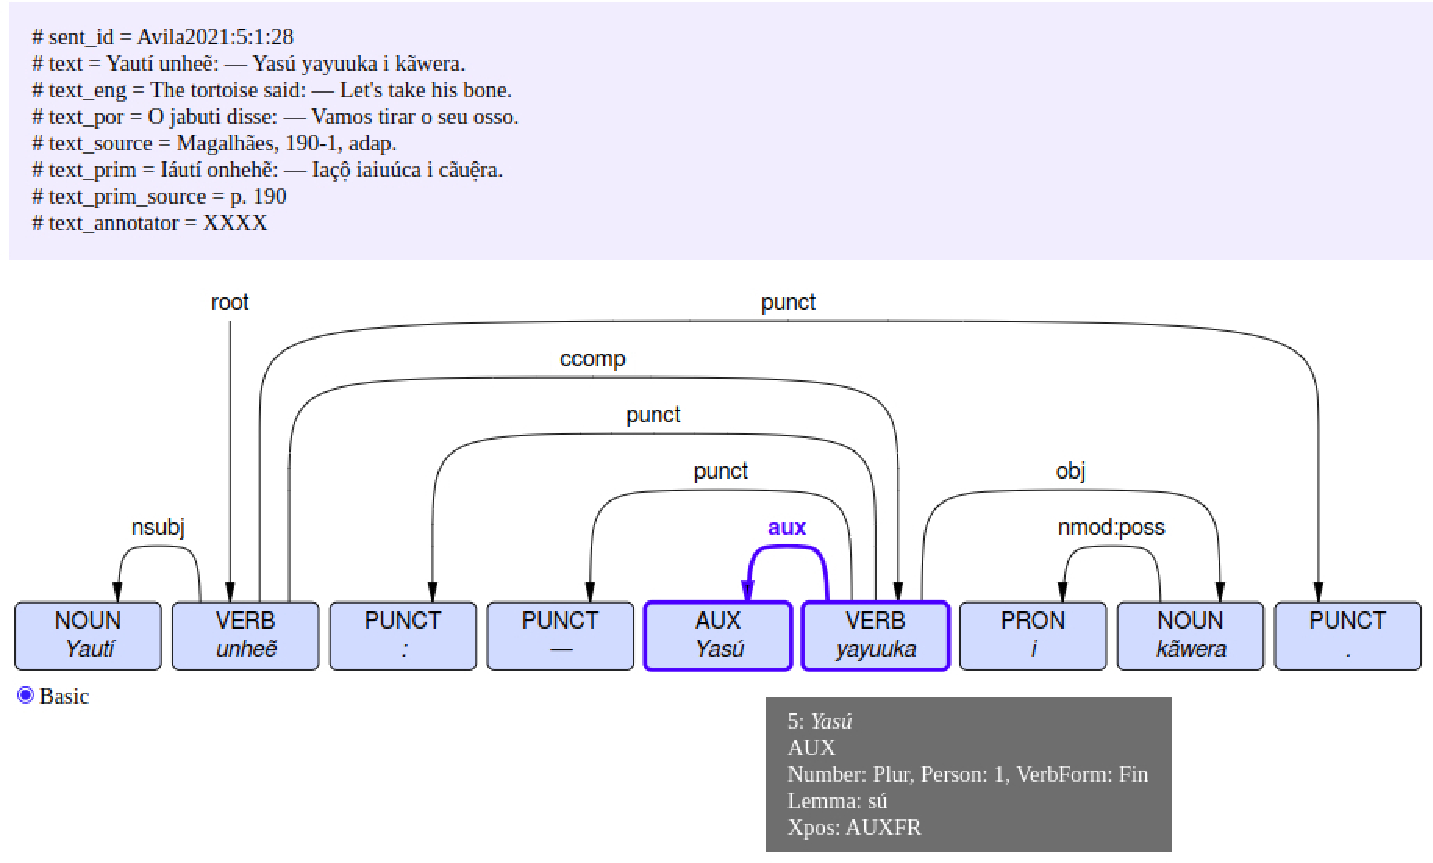
\includegraphics[width=\linewidth]{figures/aux-su.pdf}
    \caption{Representação dependencial de sentença do \tbc~com o auxiliar pré-verbal \wt{sú}{ir}.}
    \label{fig:aux-su}
    \source{Elaboração própria.}
  \end{minipage}
\end{figure}

Os traços morfossintáticos da coluna (vi), referida na documentação de UD pela abreviatura FEATS, constituem uma lista ordenada alfabeticamente de pares de atributos e valores no formato \texttt{ATRIBUTO=VALOR}, separados por $|$. Por exemplo, na coluna (vi) das linhas 2 e 3 da tabela da Figura \ref{fig:conllu}, os pares \texttt{Number=Plur}, \texttt{Person=1} e \texttt{VerbForm=Fin} especificam que se trata de formas verbais finitas na primeira pessoa do plural. O par \texttt{PronType=Prs} na coluna (vi) da linha 1 distingue os pronomes pessoais dos demais tipos de pronomes, como os demonstrativos, os interrogativos	\textit{etc.}

As informações das colunas (vii) e (viii) definem a árvore sintática dependencial, que consiste numa série de nós conectados por arcos direcionados de um nó pai regente a um nó filho dependente. Cada arco é rotulado com uma abreviatura de uma das 37 relações de dependência postuladas pela teoria UD (doravante DEPREL), como \texttt{nsubj} (sujeito nominal) e \texttt{obj} (objeto direto).

O modelo UD adota uma posição lexicalista na análise sintática. Isso significa que a menor unidade linguística do \textit{corpus} é a palavra. Unidades menores, como o prefixo \textit{ya} de primeira pessoa do plural (Figura \ref{fig:dep-tree}) ou o prefixo relacional \textit{r} de contiguidade (Figura \ref{fig:non-verbal}), não constituem nós na árvore dependencial. A contribuição desses morfemas para a representação morfossintática da sentença é codificada na estrutura de traços. As árvores sintáticas nesse modelo estabelecem, portanto, relações de dependência entre palavras (Figuras \ref{fig:dep-tree} e \ref{fig:aux-su}), ao contrário das de teorias constitucionais, que se baseiam na estrutura sintagmática, representando relações de parte e todo (Figura \ref{fig:ctree}). 

A raiz da árvore dependencial, identificada pelo índice 0, é o único nó que não representa uma palavra da frase. Trata-se de artifício que confere uma estrutura comum a todo tipo de sentença. Esse nó abstrato domina o nó da palavra hierarquicamente superior da sentença por meio da relação \texttt{root}. No caso de predicados verbais, esse nó mais alto é o único verbo pleno da oração (Figura \ref{fig:dep-tree}) ou o verbo principal (Figura \ref{fig:aux-su}). A Figura \ref{fig:non-verbal} exibe a estrutura dependencial de sentença em que o nó mais alto constitui um substantivo.  

\begin{figure}[htbp]
  \centering
  \begin{minipage}{.7\textwidth}
    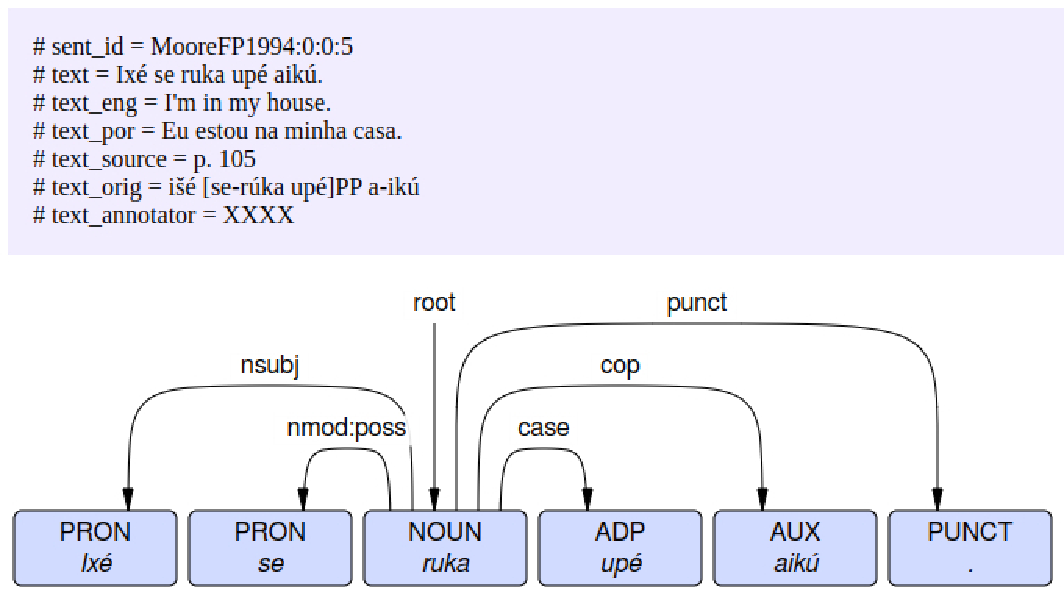
\includegraphics[width=\linewidth]{figures/non-verbal.pdf}
    \caption{Representação dependencial de sentença do \tbc~com predicado nominal.}
    \label{fig:non-verbal}
    \source{Elaboração própria.}
  \end{minipage}
\end{figure}
 

\begin{figure}[htbp]
  \centering
  \begin{minipage}{.5\textwidth}
    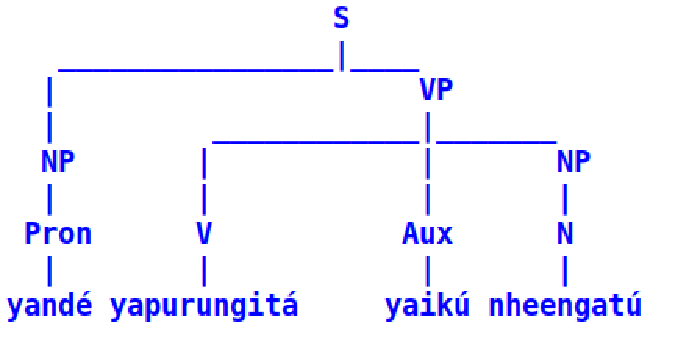
\includegraphics[width=\linewidth]{figures/ctree-ascii.pdf}
    \caption{Árvore sintagmática baseada em \textcite{moore-facundes-pires-1994} para a sentença da Figura \ref{fig:dep-tree}.}
    \label{fig:ctree}
    \source{Elaboração própria.}
  \end{minipage}
\end{figure}

O modelo UD distingue entre palavras de conteúdo, que incluem todas as classes da primeira macrocategoria da \Cref{tab:upos}, e palavras funcionais, que constituem um subconjunto próprio do conjunto definido pela segunda macrocategoria da \Cref{tab:upos}, ou seja, toda palavra funcional integra o conjunto de palavras de classe fechada, mas nem toda palavra de classe fechada é funcional \parencite{Lehmann2023-word-classes}. Esse é o caso, por exemplo, dos numerais e dos pronomes \parencite{lopes2022corpora}.\footnote{A esse respeito, o modelo UD difere de abordagens como \textcite{Lehmann2013-nature}, que trata pronomes como palavras gramaticais.} Via de regra, palavras funcionais figuram apenas como dependentes, ao passo que palavras de conteúdo tanto podem reger outras palavras quanto ser regidas \parencite{UD2024-Syntax}. Com base nessa distinção, as relações do conjunto DEPREL subdividem-se em dois grupos. O primeiro grupo consiste de relações sintáticas que se estabelecem entre duas palavras de conteúdo, por exemplo, entre dois substantivos, dois verbos ou dois numerais,\footnote{Por exemplo, em expressões como \textit{5 -- 6 metros} ou \textit{1920 x 1080 pixels} \parencite[p. 285]{de-marneffe-etal-2021-universal-k}.} entre um verbo e um substantivo ou pronome, um substantivo e um adjetivo ou um verbo e um advérbio. Além de \texttt{nsubj} e \texttt{obj}, esse grupo abarca relações como \texttt{iobj} (objeto indireto), \texttt{obl} (oblíquo), \texttt{csubj} (sujeito oracional), \texttt{ccomp} (complemento oracional), \texttt{xcomp} (complemento oracional aberto) e \texttt{nmod} (modificador nominal). O segundo grupo abrange relações sintáticas entre uma palavra de conteúdo e uma palavra funcional, como \texttt{case}, \texttt{mark} e \texttt{aux}, que se aplicam a adposições, conjunções subordinativas e auxiliares, respectivamente.

A teoria não impõe que toda língua natural possua todas as 37 relações sintáticas. Exige apenas que as relações sintáticas de uma língua constituam um subconjunto dessas relações. Por outro lado, a teoria permite que uma relação sintática seja subtipada, de modo a contemplar especificidades de uma língua. Esses subtipos podem ser criados livremente, mas precisam estar documentados no sistema de UD para serem aceitos pelo \textit{script} de validação. O \tbc~vale-se no momento de três relações subtipadas, a saber \texttt{nmod:poss}, \texttt{acl:relcl} e \texttt{advcl:relcl}, utilizadas por vários outros \textit{treebanks}. 

A última coluna da tabela da Figura \ref{fig:conllu}, denominada MISC, abriga quaisquer informações adicionais que construtores de um \tb~julguem relevantes. Seguindo vários \tbs~d\cdc, o \tbc~inclui nesse campo, entre outros, os atributos Space\-After e Token\-Range. O primeiro indica a ausência de espaço em branco subseguindo o \textit{token}. O segundo atributo indica a posição inicial e final do \textit{token} na cadeia de caracteres (\textit{string}) por meio da notação \texttt{n:m}, adotada na linguagem de programação Python, onde \texttt{n} é o índice do primeiro caractere do \textit{token} e \texttt{m-1}, do último. 

\section{Metodologia de construção do corpus}\label{sec:metodologia}

\subsection{O material linguístico}\label{subsec:material}

Nesta seção, tratamos do material linguístico que compõe a versão atual do \tbc, ao qual continuamente novos exemplos se agregam. No momento, as sentenças do \tb~provêm de 20 publicações, a maior parte das quais documentam a história do nheengatu de meados do século XIX à segunda década do XXI. Exemplos de outras publicações, como \textcite{goes2015novo}, \textcite{Avila2016} e \textcite{Trevisan2017} serão igualmente incorporados ao \tb. Extrapolaria o âmbito deste artigo discorrer pormenorizadamente sobre cada uma dessas fontes. Para tanto, remetemos o leitor a \textcite{avila2021}, que faz um levantamento detalhado dos registros escritos da LGA do século XVIII às duas primeiras décadas do século XXI. Das fontes nominadas na Figura \ref{fig:freqsources}, \textcite{moore-facundes-pires-1994} e \vum~são as únicas que não integram o corpus histórico-filológico de \textcite{avila2021}.  

\begin{figure}[htbp]
  \centering
  \begin{minipage}{.8\textwidth}
    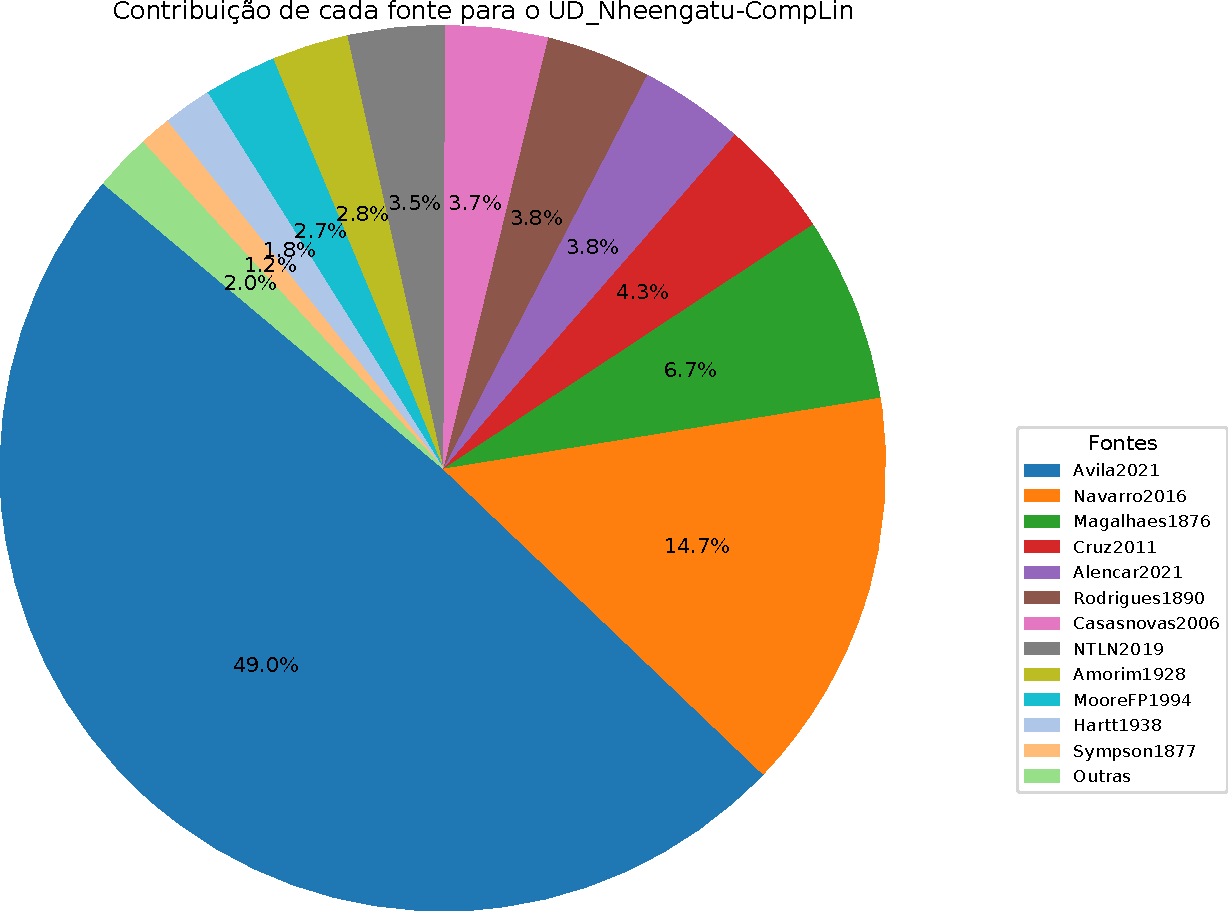
\includegraphics[width=\linewidth]{figures/FreqSources16NTB.pdf}
    \caption{Frequência relativa das principais fontes bibliográficas do \tbc. A categoria \textit{Outras} engloba fontes com menos de 16 sentenças no \tb.}
    \label{fig:freqsources}
    \source{Elaboração própria.}
  \end{minipage}
\end{figure}

Os~\tbs~da~\udc~de algumas das línguas majoritárias mais ricas em recursos para o PLN, como, por exemplo, alemão, japonês, checo, russo, português e árabe, possuem cada um mais de um milhão de palavras, os três primeiros mais que o dobro disso. No caso de uma língua que, apesar dos mais de 300 anos de história, só mais recentemente iniciou uma tradição escrita própria (os textos anteriores constituindo na maioria das vezes registros de falantes não nativos), um \tb~à altura dos dessas línguas teria de abranger todos os registros históricos acessíveis e toda ou quase toda a produção dos últimos anos.

Para dar uma ideia da relativa escassez de textos em nheengatu, a tradução do Novo Testamento \parencite{novo-testamento-nyengatu}, publicada pela primeira vez em 1973, constituindo, ao que tudo indica, o texto mais longo do nheengatu do século XX, possui pouco mais de 150.000 palavras. Publicações mais recentes, como o livreto de fábulas contadas por membros da Comunidade de Terra Preta \parencite{fabulas2013}, com cerca de 2.500 palavras em nheengatu, não alcançam uma fração ínfima dessa quantidade.

Desse modo, o ideal seria incluir no \tbc~todos os textos disponíveis. No entanto, como as ferramentas de processamento computacional do nheengatu ainda não estão suficientemente maduras ao ponto de automatizar de forma mais significativa a anotação do \textit{corpus}, esse objetivo não é realista a um curto ou médio prazo. Um outro fator a ser levado em conta é que os textos de publicações mais recentes são protegidos pelo direito autoral, não podendo ser incorporados irrestritamente ao \tb, como é o caso das fábulas referidas, cuja reprodução necessita de autorização por escrito da comunidade responsável. Por outro lado, muitas publicações não estão em formato digital pesquisável, necessitando de transcrição manual, v.g., \textcite{costa1909}, enquanto a maioria das que se encontram nesse formato demandam uma série de intervenções manuais na preparação do texto para anotação (Seção \ref{subsec:processo}). Outra dificuldade para a construção de \textit{corpora} anotados e a implementação de ferramentas de processamento é a gigantesca diversidade de ortografias do nheengatu.

Dadas essas limitações, dividimos a construção do \tbc~em diversas etapas. Para a etapa objeto deste artigo, selecionamos primeiramente exemplos que permitissem fornecer uma visão geral da estrutura morfossintática do nheengatu sob a perspectiva do modelo UD, aproveitando as publicações mais acessíveis e atentando para as questões de direito autoral. Outro critério decisivo que permeou essas escolhas foi o grau de facilidade de anotação, determinado por fatores como a disponibilidade e o tipo de versão digital do texto, a qualidade das traduções e o detalhamento da análise lexical e/ou gramatical prévia, principalmente sob a forma de glosas interlineares. Com base nesses critérios, compilamos e anotamos o primeiro grupo de exemplos, extraídos de \textcite{moore-facundes-pires-1994}, \textcite{cruz2011}, \textcite{navarro2016}, \vum~e \textcite{avila2021}. O segundo grupo de exemplos visou a antecipar os diversos problemas a serem enfrentados nas etapas seguintes. Para tanto, incorporamos progressivamente exemplos de variadas fontes, tanto sentenças individuais quanto passagens mais extensas ou textos inteiros, representativos do tesouro textual do nheengatu de meados do século XIX aos dias de hoje, norteando-nos principalmente pelo abrangente levantamento de fontes que embasam o dicionário de \textcite{avila2021}. 

A Figura \ref{fig:size-stats} sumaria alguns dos principais dados quantitativos que permitem dimensionar o tamanho atual do \tbc~e compará-lo com os outros cinco maiores \tbs~de línguas ameríndias na versão v.2.14 da \udc.\footnote{As Figuras \ref{fig:size-stats}, \ref{fig:treebank-stats}, \ref{fig:tag-freq} e \ref{fig:rel-tag-freq} condensam dados gerados pelo \textit{script} \href{https://github.com/UniversalDependencies/tools/blob/master/conllu-stats.pl}{conllu-stats.pl}, compilados no arquivo \texttt{stats.xml} do repositório de cada \tb.} O gráfico evidencia que o \tbc~supera significativamente os demais no número de palavras, consistindo, também, do maior número de sentenças. Quanto ao número de lemas e formas, o \tbc~se aproxima dos \tbs~que ocupam a primeira posição nessas duas dimensões.

\begin{figure}[htbp]
  \centering
  \begin{minipage}{.9\textwidth}
    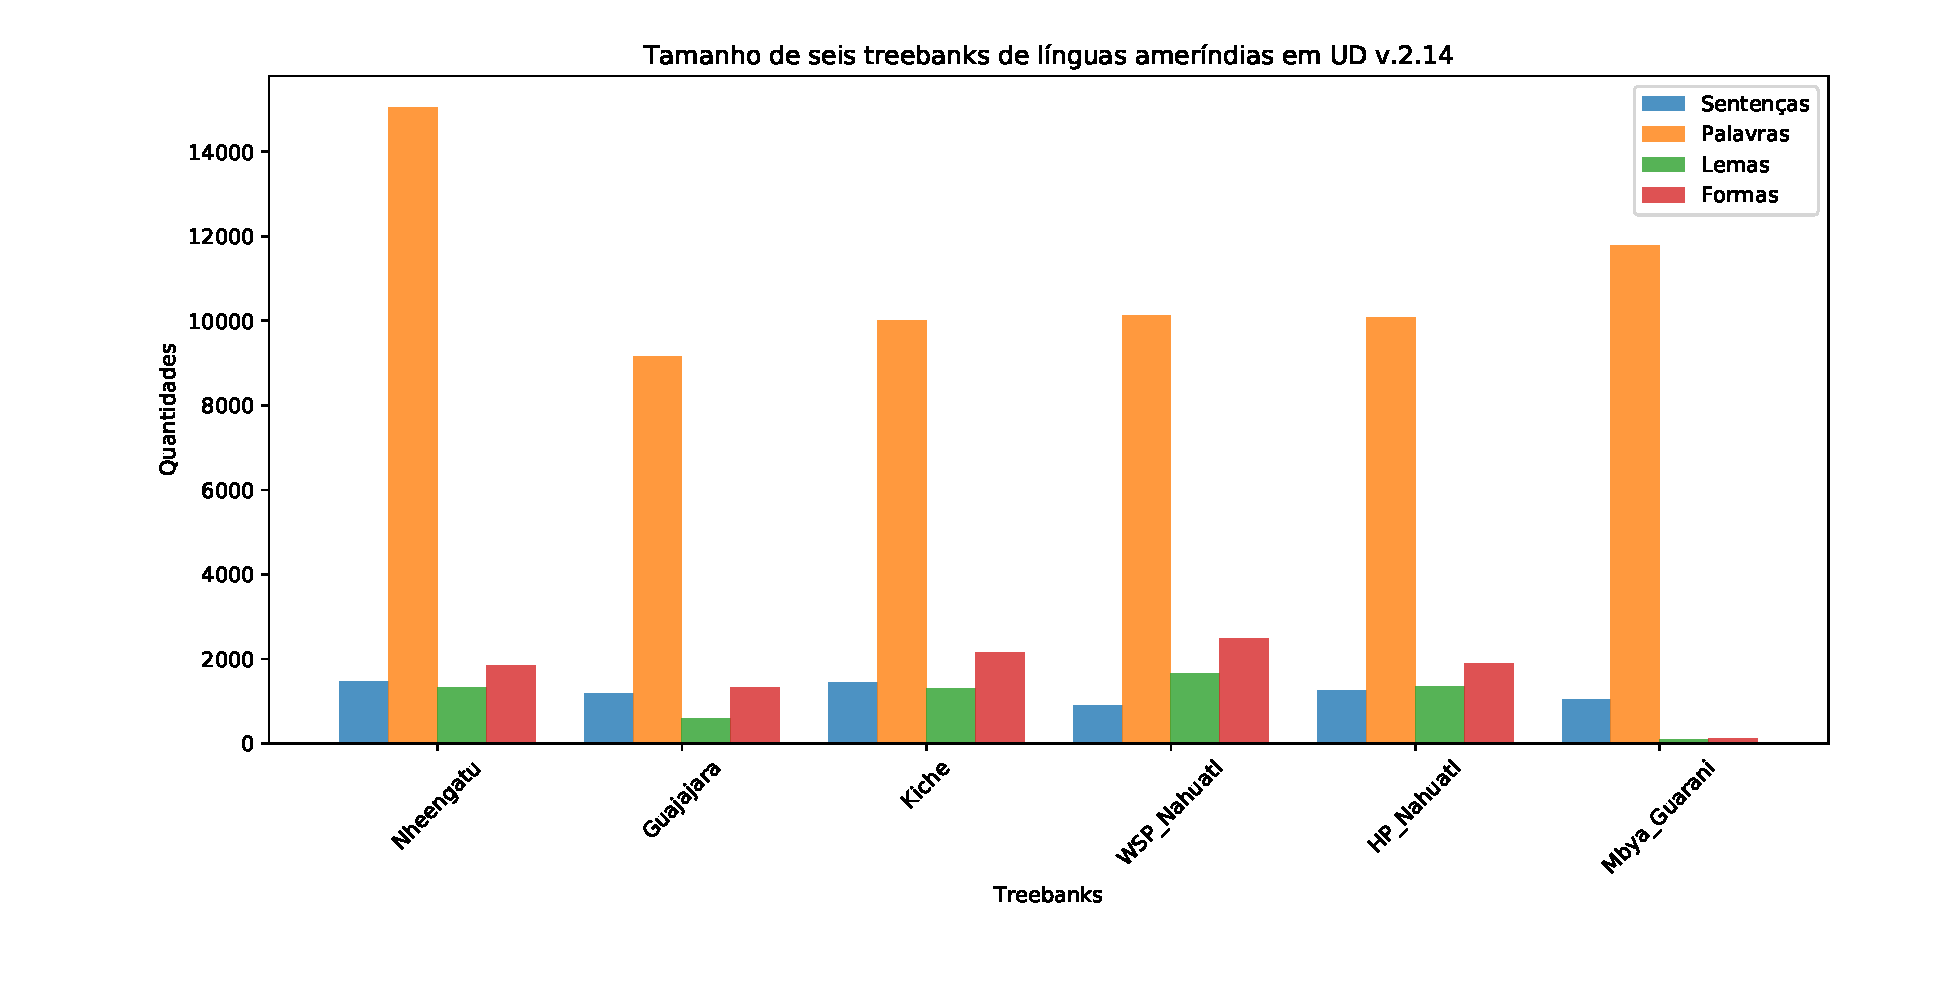
\includegraphics[width=\linewidth]{figures/TreebankSizeStats.pdf}
    \caption{Dados quantitativos dos seis maiores \tbs~de línguas ameríndias em UD v.2.14.}
    \label{fig:size-stats}
    \source{Elaboração própria a partir dos dados de \textcite{zeman2024universal}.}
  \end{minipage}
\end{figure}

\begin{figure}[htbp]
  \centering
  \begin{minipage}{.75\textwidth}
    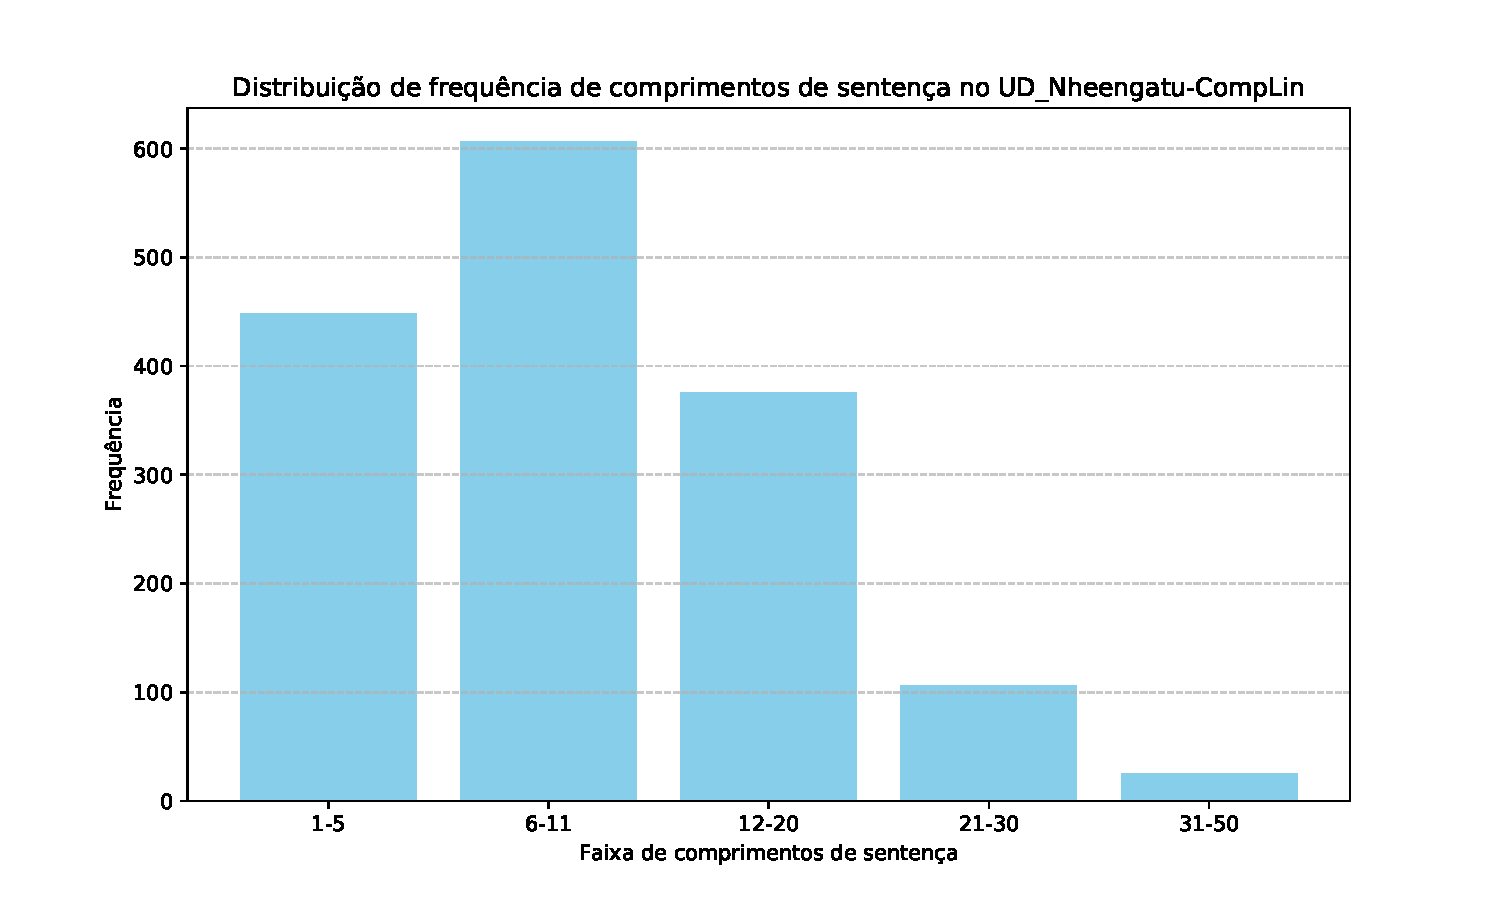
\includegraphics[width=\linewidth]{figures/SentLensNheenRangesPor.pdf}
    \caption{Comprimentos de sentença por quantidade de palavras no \tbc.}
    \label{fig:comprimentos}
    \source{Elaboração própria.}
  \end{minipage}
\end{figure}

A Figura \ref{fig:comprimentos} evidencia que o \tb~possui uma distribuição diversificada de tipos de sentença em termos de extensão, incluindo tanto sentenças curtas como muitas bastante longas, com 355 sentenças na faixa de 12 a 20 palavras e 126 entre 21 e 49, perfazendo uma média de 10,23 palavras por sentença com desvio padrão de 6,93 e uma mediana de 8,0.\footnote{Valores computados por meio das funções correspondentes da biblioteca \href{https://numpy.org/}{numpy} de Python, aplicadas sobre uma lista com as quantidades de palavras sintáticas das 1.470 sentenças do \tb.}

Constatamos na Figura \ref{fig:freqsources} que quase metade dos exemplos consiste de abonações dos verbetes de \textcite{avila2021}. Totalizando 15\% do \tb, o segundo maior grupo de exemplos provém de \textcite{navarro2016}, um curso dividido em 13 lições, obedecendo a uma progressão gramatical que cobre uma ampla parcela da estrutura morfossintática da língua, exemplificada tanto por trechos ou textos completos adaptados da literatura, como \textcite{magalhaes1876}, \textcite{rodrigues1890}, \textcite{stradelli1929}, \textcite{Amorim1928} e \textcite{cruz2011}, quanto por textos construídos. Um glossário de mais de 800 entradas indica as classes de palavra, propriedades flexionais e acepções do vocabulário desses textos, que podem ser extraídos de arquivo no formato PDF e preparados para anotação automática com poucas intervenções manuais.  

Com cerca de 8.000 verbetes, dos quais aproximadamente 6.400 consistem em entradas principais e 1.600 em variantes, \textcite{avila2021} é o mais abrangente dicionário do nheengatu de que se dispõe. Fundamenta-se num conjunto de publicações diatópica e diacronicamente representativo, estendendo-se sobretudo de meados do século XIX à segunda década de XXI, complementado por dados coletados junto a informantes na região do Alto Rio Negro. A microestrutura dos verbetes contempla uma ampla gama de informações, incluindo a etimologia, as marcas de uso, especificações morfossintáticas como classe de palavra e regência, as diferentes acepções e subacepções, os lemas tanto atuais quanto históricos e os registros na literatura antiga com as respectivas variantes ortográficas (Figura \ref{fig:verbetes}). Via de regra, não só as lexias simples e complexas, mas também afixos flexionais e derivacionais de todos os exemplos correspondem a lemas do dicionário. Também são consignadas várias centenas de derivados, compostos e locuções de diversas classes de palavras.

Ao todo, abonam os verbetes mais de 4.000 exemplos diferentes, a maioria provenientes da literatura, com apenas cerca de 10\% da lavra do próprio dicionarista. As abonações obedecem a uma formatação sistemática, constituída de três partes, a saber, (i) sentença nheengatu, (ii) fonte e (iii) tradução portuguesa, o que facilita a geração automática de parte substantiva dos metadados da anotação. Como podemos constatar na Figura \ref{fig:peteka-idle}, alimentado com uma abonação de \textcite{avila2021}, o Yauti\footnote{Disponível no repositório \url{https://github.com/CompLin/nheengatu}.} automaticamente constrói os valores dos atributos \texttt{text}, \texttt{text\_source} e \texttt{text\_por}, do último dos quais se vale, via tradutor do Google™, para preencher o atributo \texttt{text\_eng}.

\begin{figure}[htbp]
  \centering
  \begin{minipage}{.75\textwidth}
    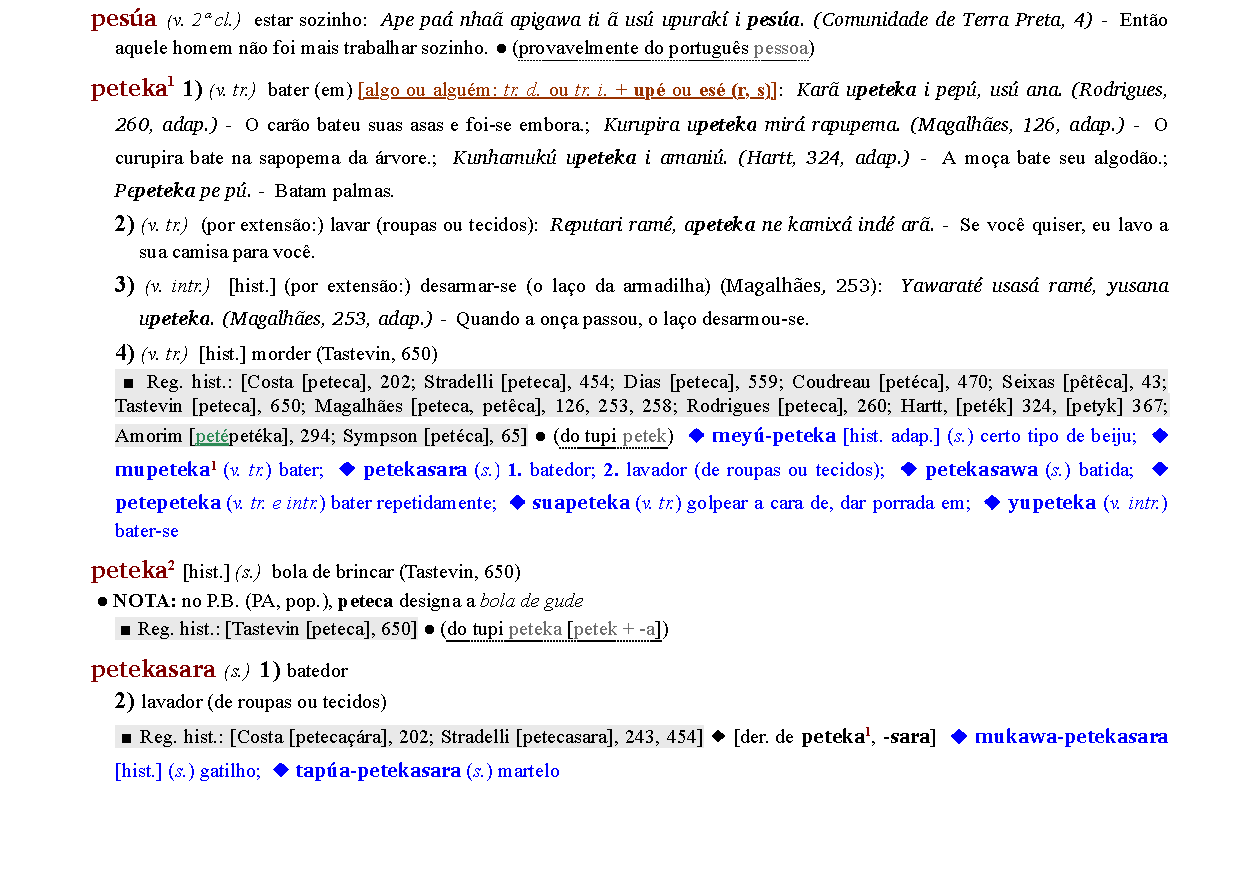
\includegraphics[width=\linewidth]{figures/2021_MarcelTwardowskyAvila_VCorr_p593_excerpt.pdf}
    \caption{Excerto de \textcite[p. 592]{avila2021}.}
    \label{fig:verbetes}
    \source{Elaboração própria por meio de recorte de página em PDF.}
  \end{minipage}
\end{figure}

Outro ponto forte do dicionário é que transcende o domínio lexicográfico propriamente dito, uma vez que as informações gramaticais do corpo principal de algumas dezenas de verbetes são complementadas por explicações gramaticais sob a forma de notas, algumas delas bastante extensas. Diversos temas da gramática do nheengatu são aprofundados, tanto do ponto de vista sincrônico quanto diacrônico, em anexos ou no corpo principal da tese que ensejou o dicionário. 
Todas essas características fazem de \textcite{avila2021} a publicação em nheengatu mais adequada para a rápida construção de um \tb~ conforme a teoria UD.  

\begin{figure}[htbp]
  \centering
  \begin{minipage}{.75\textwidth}
    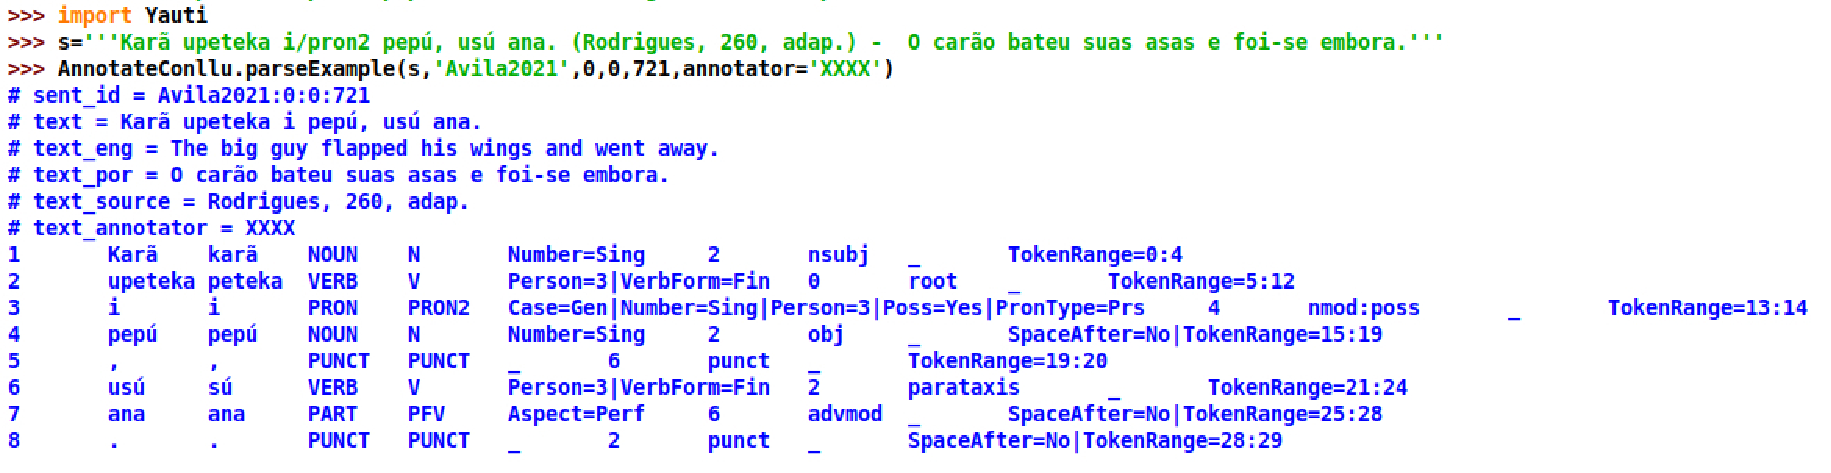
\includegraphics[width=\linewidth]{figures/peteka-idle.pdf}
    \caption{Geração de metadados e análise morfossintática com o Yauti a partir de exemplo do verbete \textbf{peteka$^1$} da Figura \ref{fig:verbetes}.}
    \label{fig:peteka-idle}
    \source{Elaboração própria.}
  \end{minipage}
\end{figure}

\begin{figure}[htbp]
  \centering
  \begin{minipage}{.8\textwidth}
    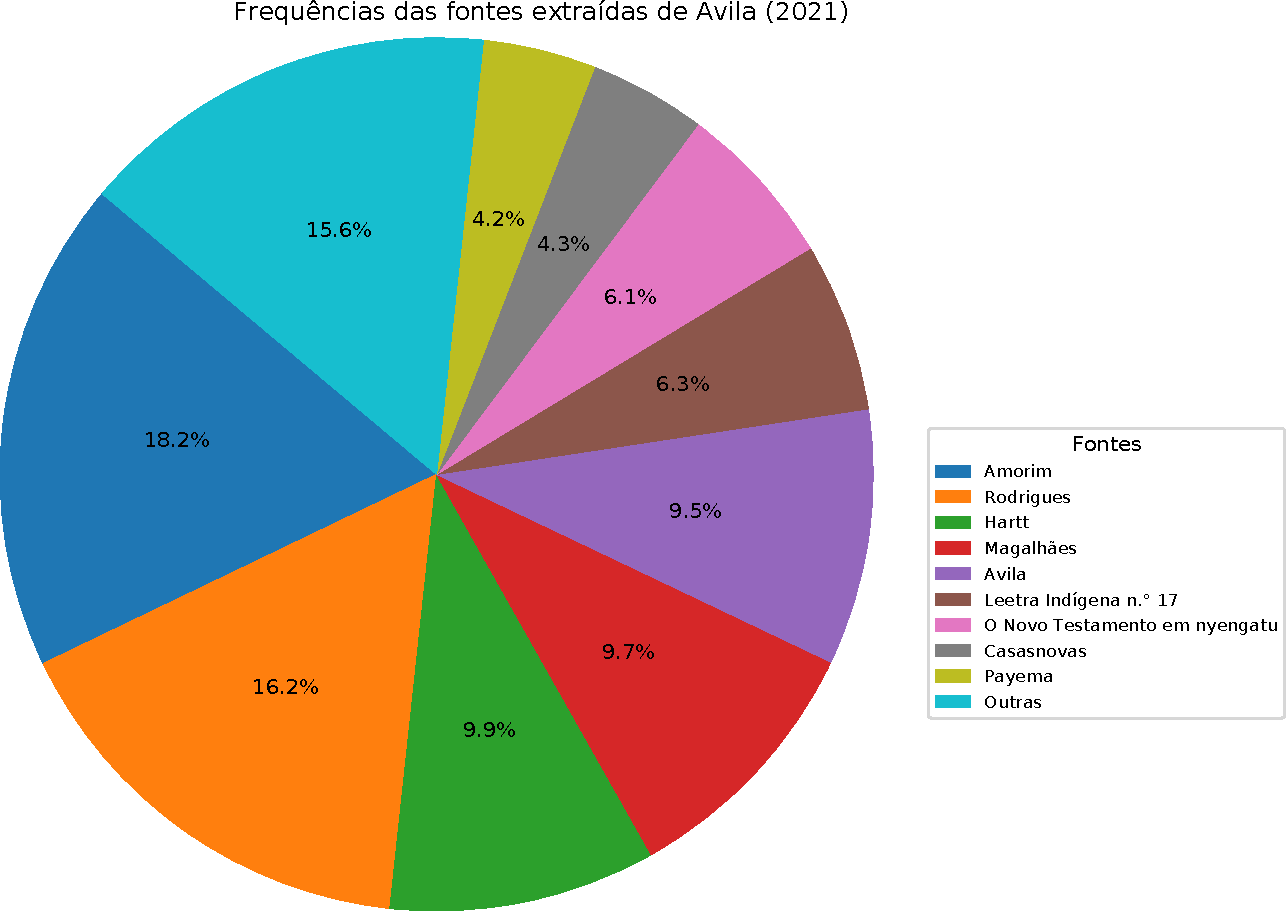
\includegraphics[width=\linewidth]{figures/FreqSourcesAvila.pdf}
    \caption{Frequência relativa das fontes bibliográficas de \textcite{avila2021} utilizadas no \tbc. A categoria \textit{Outras} engloba fontes com menos de 30 sentenças no \tb.}
    \label{fig:freqsources-avila}
    \source{Elaboração própria.}
  \end{minipage}
\end{figure}

\subsection{A normalização ortográfica}\label{subsec:normal}

A normalização ortográfica é um procedimento padrão na linguística de \textit{corpus} \parencite{hirschmann2019korpuslinguistik}. Num \tb~do nheengatu, essa questão é crucial, haja vista a inexistência de uma ortografia uniforme. Talvez não seja exagero afirmar que cada publicação em nheengatu adota um padrão próprio, ainda assim, dentro de determinadas obras, deparamo-nos com significativa variação grafêmica \parencite{avila2021,DAngelis-2023}. A discrepância entre as grafias de uma mesma palavra chega a ser tão extrema ao ponto de não compartilharem caractere algum, como, por exemplo, \textit{yã} relativamente a \textit{nhan}, \textit{nhaan} e \textit{naa}, algumas das variantes de \wt{nhaã}{aquele}. Sem uma normalização ortográfica, seria impraticável a um usuário do \tb~recuperar todas as ocorrências desse pronome demonstrativo. Uma complicação adicional é que as diferenças ortográficas não se limitam à representação de fonemas, estendendo-se à segmentação de palavras. Esse tipo de variação é pervasivo nos textos nheengatus, afetando diferentes morfemas, escritos ora separados, ora juntos da palavra anfitriã, intermediados ou não por hífen, como o relativizador \textit{waá} (grafado também \textit{ua}, \textit{uaa}, \textit{uá}, \textit{uahá}, \textit{wa} 	\textit{etc.})

No \tbc, \texttt{text} assinala a versão normalizada do texto original, preservado \textit{ipsis litteris} como valor do atributo \texttt{text\_orig} (Figuras \ref{fig:dep-tree} e \ref{fig:non-verbal}). Em exemplos de \textcite{avila2021} provenientes da literatura nheengatu, o atributo \texttt{text\_prim} reproduz o texto primário (Figuras \ref{fig:aux-su} e \ref{fig:style-arch}). A exemplo do anotador morfossintático Yauti \pvtres, adotamos na normalização ortográfica a proposta de \textcite{avila2021}, dada a abrangência diacrônica e sincrônica desse dicionário. Cumpre salientar, no entanto, que essa escolha não representa, absolutamente, um juízo de valor de que essa ortografia é melhor do que as outras. De fato, \textcite{avila2021}  propõe esse padrão com a única finalidade de facilitar a consulta ao dicionário. Trata-se de estratégia análoga à ortografia de trabalho definida por \textcite{DAngelis-2021}.
	 
\subsection{O processo de anotação e revisão}\label{subsec:processo}
Nesta subseção, tratamos das diferentes tarefas envolvidas na inclusão de uma nova sentença no \tbc, as quais se articulam no fluxograma da Figura \ref{fig:fluxograma-anotacao}.

\begin{figure}[htbp]
  \centering
  \begin{minipage}{.9\textwidth}
    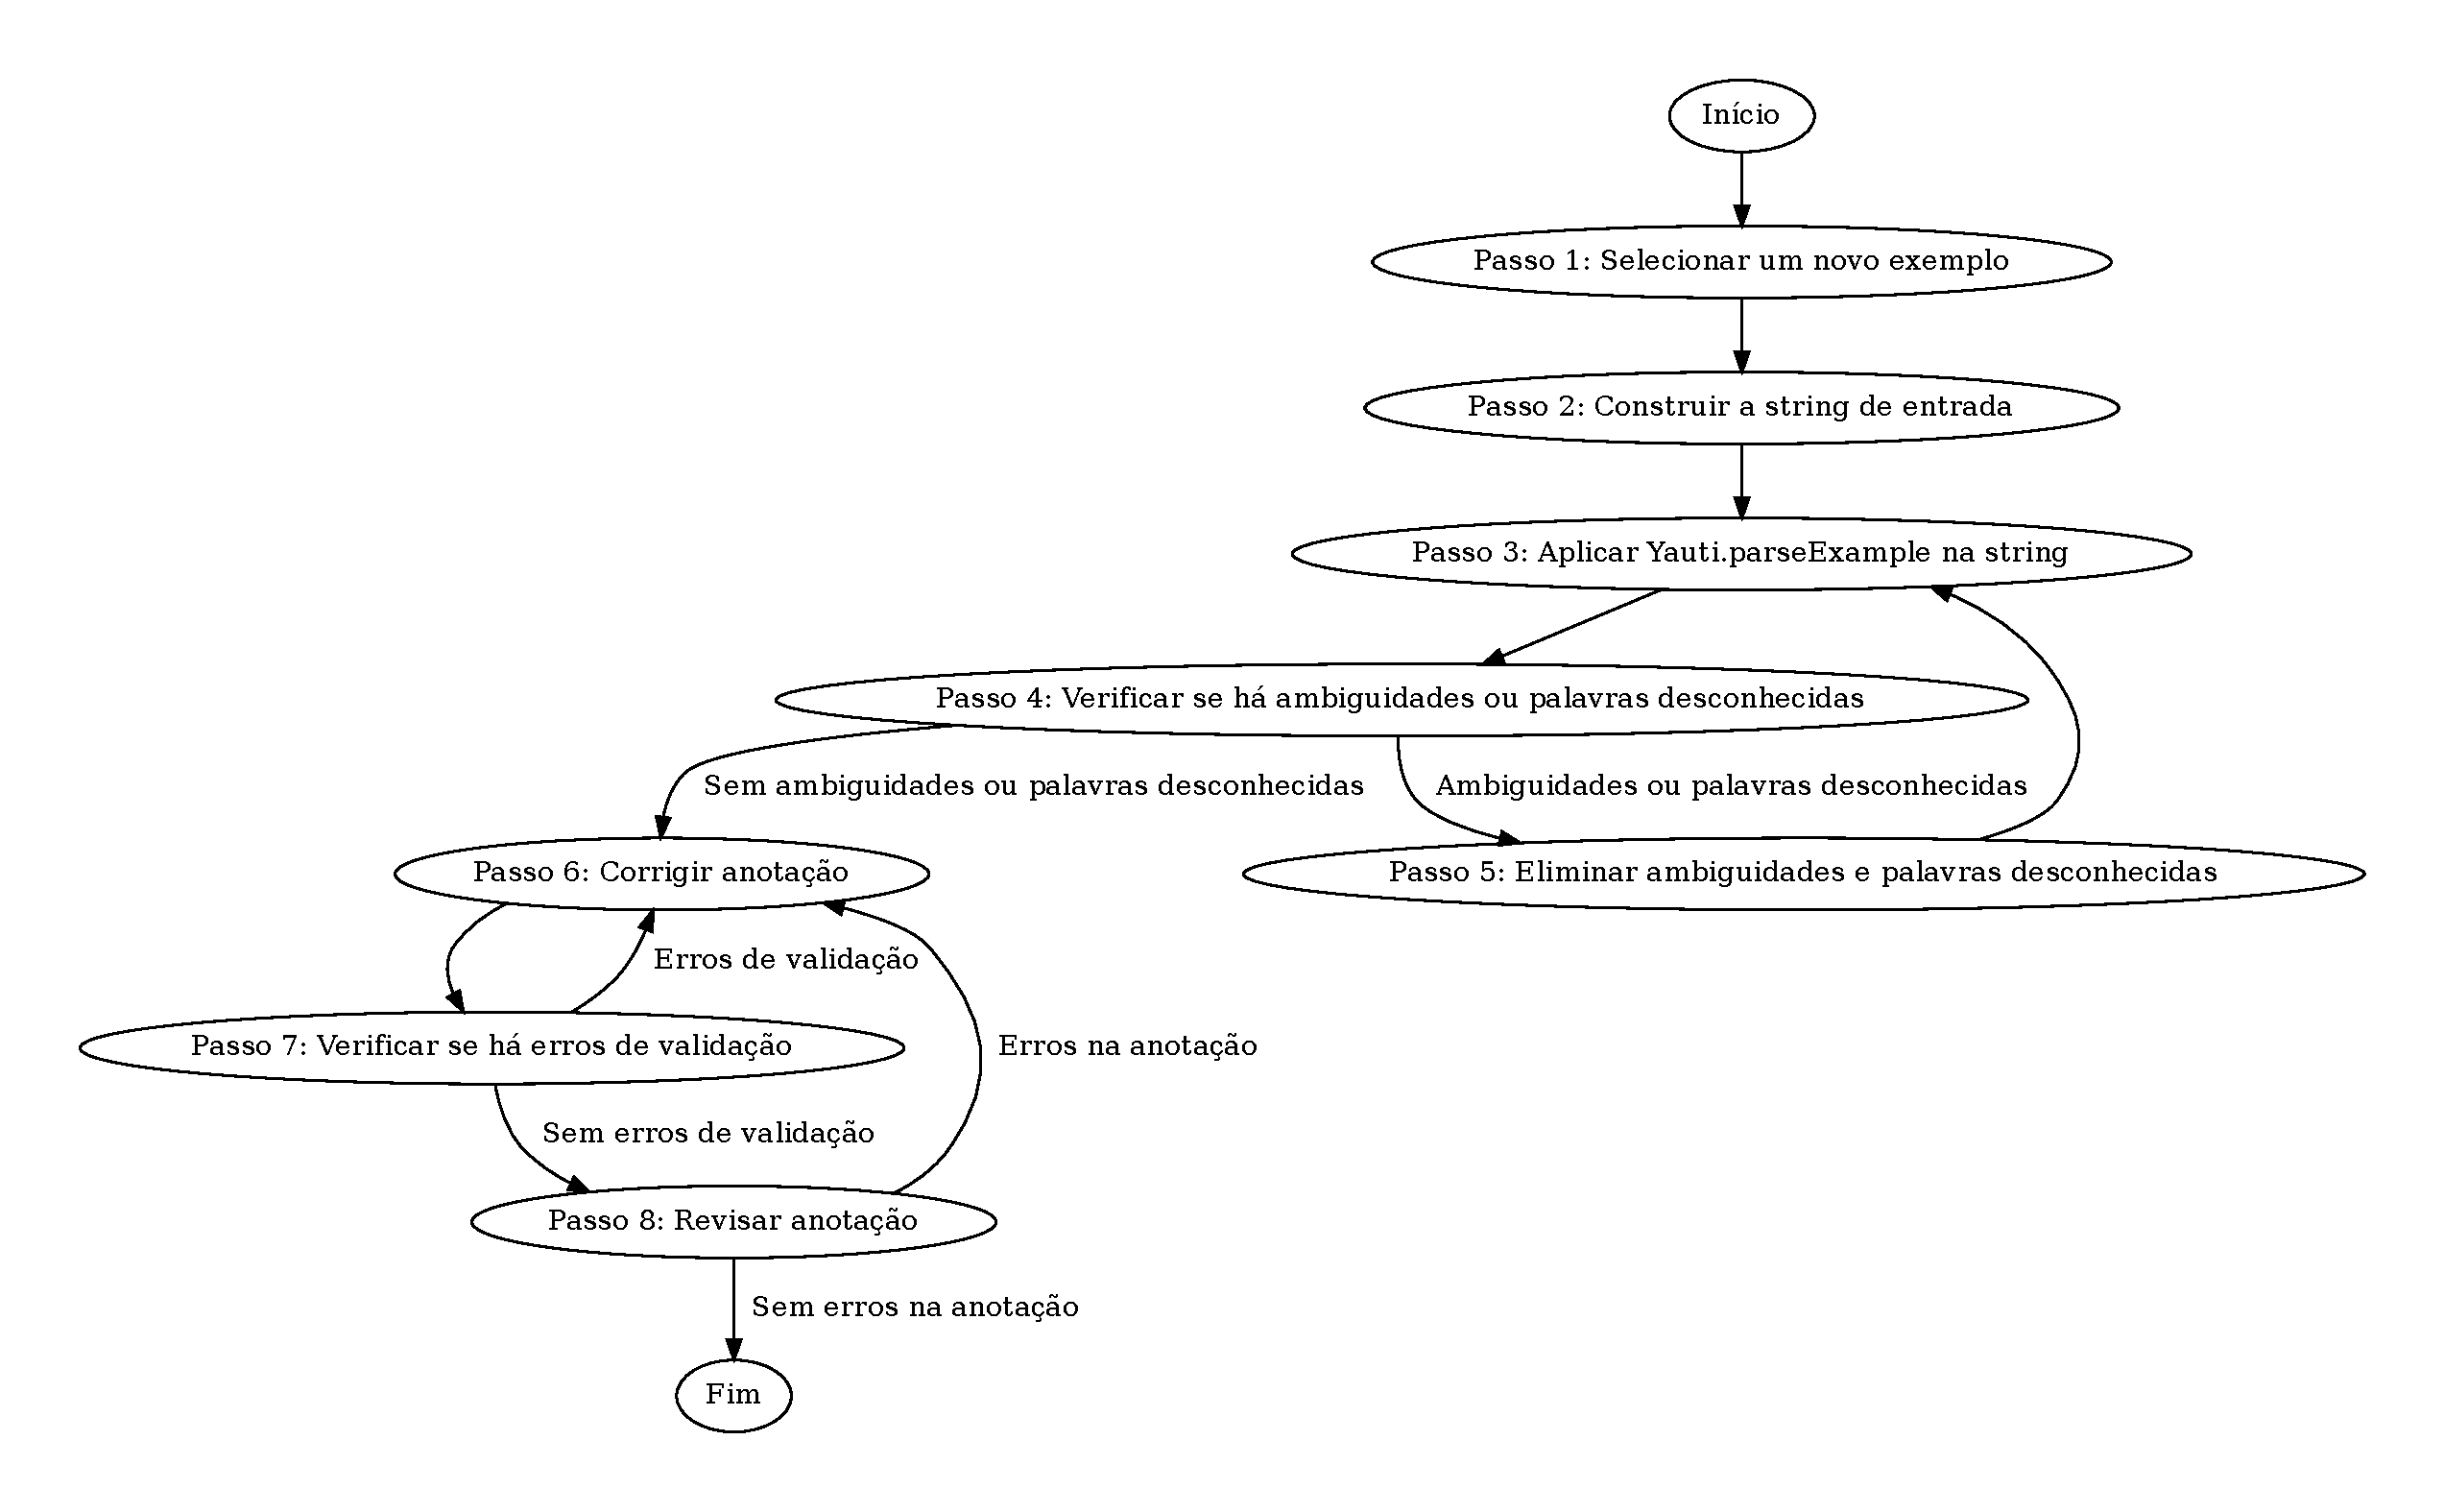
\includegraphics[width=\linewidth]{figures/fluxo-anotacao-1.pdf}
    \caption{Fluxograma da inclusão de uma nova sentença anotada no \tbc.}
    \label{fig:fluxograma-anotacao}
    \source{Elaboração própria.}
  \end{minipage}
\end{figure}

Nosso objetivo de longo prazo é abarcar com o \tb~todo o material textual nheengatu em domínio público, além de textos de cujos proprietários venhamos a obter permissão. Visando a metas de curto prazo de expansão do \tb~relacionadas às \textit{releases} periódicas da \udc, distinguimos duas situações típicas que se deparam no primeiro passo do fluxograma da Figura \ref{fig:fluxograma-anotacao}.

A primeira situação configura-se quando se trata de anotar todas as sentenças de uma dada publicação ou de uma ou mais narrativas ou trechos contínuos. Nesse caso, anotamos os exemplos, via de regra, na sequência em que aparecem na respectiva fonte. A segunda situação ocorre quando o objetivo é anotar sentenças com uma determinada palavra ou construção. Por exemplo, as orações relativas constituem uma das construções fundamentais do nheengatu. Desse modo, um \textit{parser} capaz de analisar corretamente os diferentes tipos de estruturas com o relativizador \textit{waá} precisa ser treinado num \tb~com um grande número de variados exemplos com esse elemento. Para tanto, extraímos sentenças com \textit{waá} de diferentes exposições gramaticais, como as de \textcite{seixas1853}, \textcite{magalhaes1876}, \textcite{sympson1877} e \textcite{casasnovas2006}, para somarem-se às sentenças com esse subordinador incluídas pela primeira via.

O Yauti \pvtres~foi utilizado desde o início para anotar as sentenças do \tbc~e teve seu desenvolvimento guiado pelas necessidades da anotação, crescendo em abrangência paralelamente ao \tb. Em ambas as situações delineadas acima, comumente nos deparamos com palavras ainda não codificadas no léxico da ferramenta e fenômenos gramaticais ainda não implementados cuja análise sob a perspectiva de UD e codificação em Python implicaram anotar um variado leque de exemplos característicos, de modo também a testar a respectiva implementação. Como o léxico do Yauti ainda é limitado \pvtres, ao incluir uma nova entrada no glossário da ferramenta para poder analisar um dado exemplo, aproveitamos para anotar o máximo de novos exemplos de \textcite{avila2021} com essa palavra, exemplos esses que, com frequência, continham palavras ainda não implementadas, resultando na anotação de mais sentenças, num efeito em cadeia.

A seguir, explicamos os passos de 2 a 8 da Figura \ref{fig:fluxograma-anotacao} com base num exemplo concreto. No passo 2, preparamos a \textit{string} de Python a ser dada como primeiro argumento da função \texttt{parseExample} do Yauti, conforme exemplificamos anteriormente na Figura \ref{fig:peteka-idle} com abonação de \textcite{avila2021}. Em exemplos de \textcite{magalhaes1876} e \textcite{sympson1877}, como de publicações análogas, atualizamos a ortografia da tradução em português e adaptamos o texto original à proposta ortográfica de \textcite{avila2021}, incluindo-o como último componente da referida \textit{string} (Figura \ref{fig:unknown-word-idle}). 

\begin{figure}[htbp]
  \centering
  \begin{minipage}{.75\textwidth}
    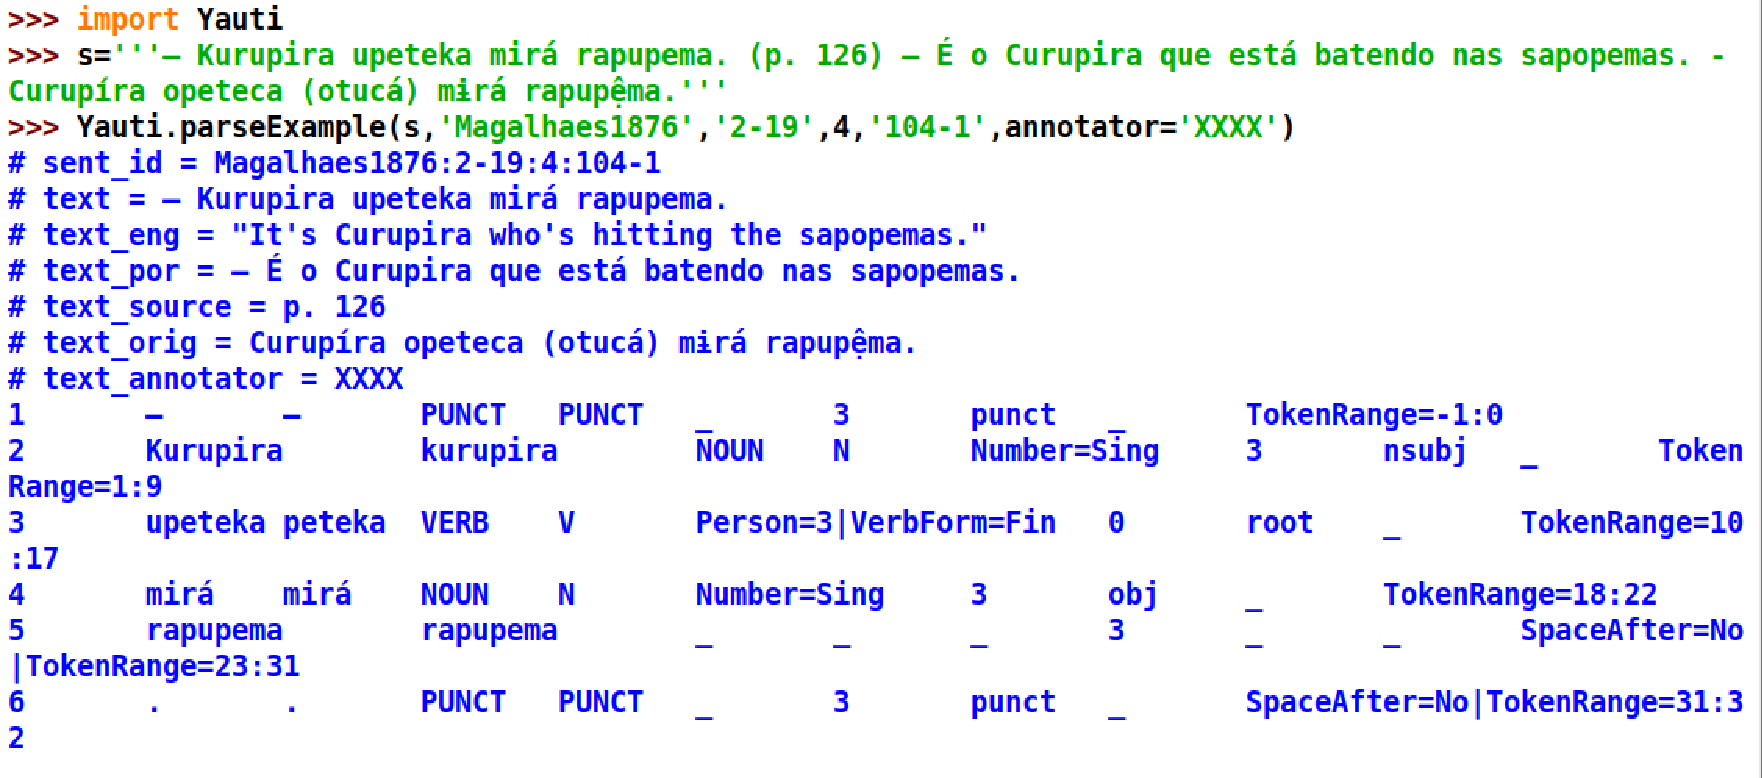
\includegraphics[width=\linewidth]{figures/unknown-word-idle.pdf}
    \caption{Preparação de exemplo de \textcite[p. 126]{magalhaes1876} e primeira aplicação da função \texttt{parseExample} do Yauti.}
    \label{fig:unknown-word-idle}
    \source{Elaboração própria.}
  \end{minipage}
\end{figure}

Nos passos 3 e 4, executamos a função \texttt{parseExample}, constatando que o Yauti não reconheceu o quinto \textit{token} da sentença (Figura \ref{fig:unknown-word-idle}). Isso ocorreu porque o seu léxico ainda não incluía essa palavra, consignada em \textcite{avila2021}. Realizada a atualização da ferramenta, conforme o passo 5, reexecutamos a função \texttt{parseExample}, gerando a análise da Figura \ref{fig:upeteka-magalhaes-idle}. No passo 6, analisamos essa anotação, recorrendo, geralmente, a uma ferramenta de visualização de árvores no formato \conll~(Figura \ref{fig:upeteka-tree}). Nesse exemplo, apenas a tradução automática do português para o inglês necessitou correção. O passo 7 consiste na aplicação do \textit{script} \href{https://github.com/UniversalDependencies/tools/blob/master/validate.py}{validate.py}, ferramenta do projeto UD que verifica se uma análise no formato \conll~obedece a uma série de requisitos do modelo \parencite{UDValidation2024}, como exemplificado na Figura \ref{fig:validation} com duas outras sentenças. Como o \textit{script} considera válida a análise da Figura \ref{fig:upeteka-magalhaes-idle}, concluímos o ciclo com o passo 8, que consiste na revisão da anotação por um outro anotador. Divergindo anotador inicial e revisor, procedemos à adjudicação das discrepâncias \parencite{hirschmann2019korpuslinguistik}.\footnote{\vquatro~pormenoriza a composição da equipe de anotadores e revisores.}  

\begin{figure}[htbp]
  \centering
  \begin{minipage}{.75\textwidth}
    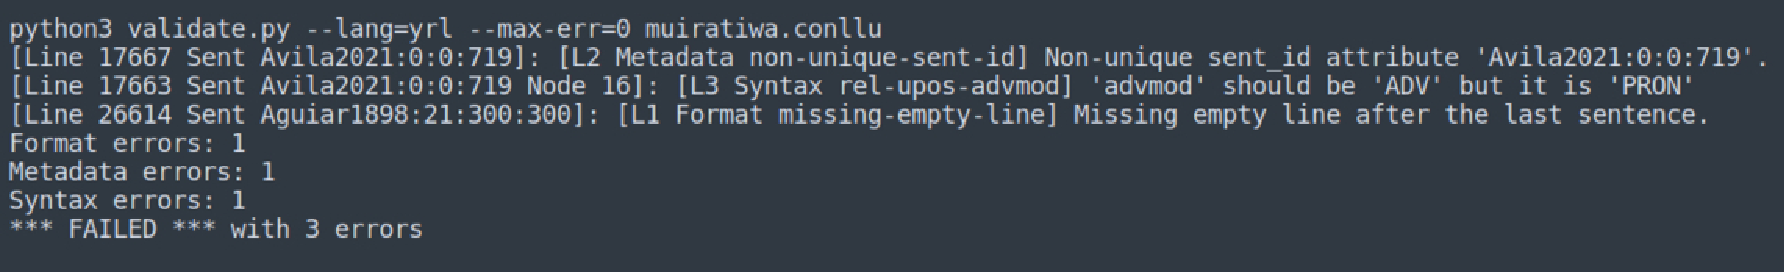
\includegraphics[width=\linewidth]{figures/validator.pdf}
    \caption{Detecção de erros de validação por meio do \textit{script} \href{https://github.com/UniversalDependencies/tools/blob/master/validate.py}{validate.py}.}
    \label{fig:validation}
    \source{Elaboração própria.}
  \end{minipage}
\end{figure}

\begin{figure}[htbp]
  \centering
  \begin{minipage}{.75\textwidth}
    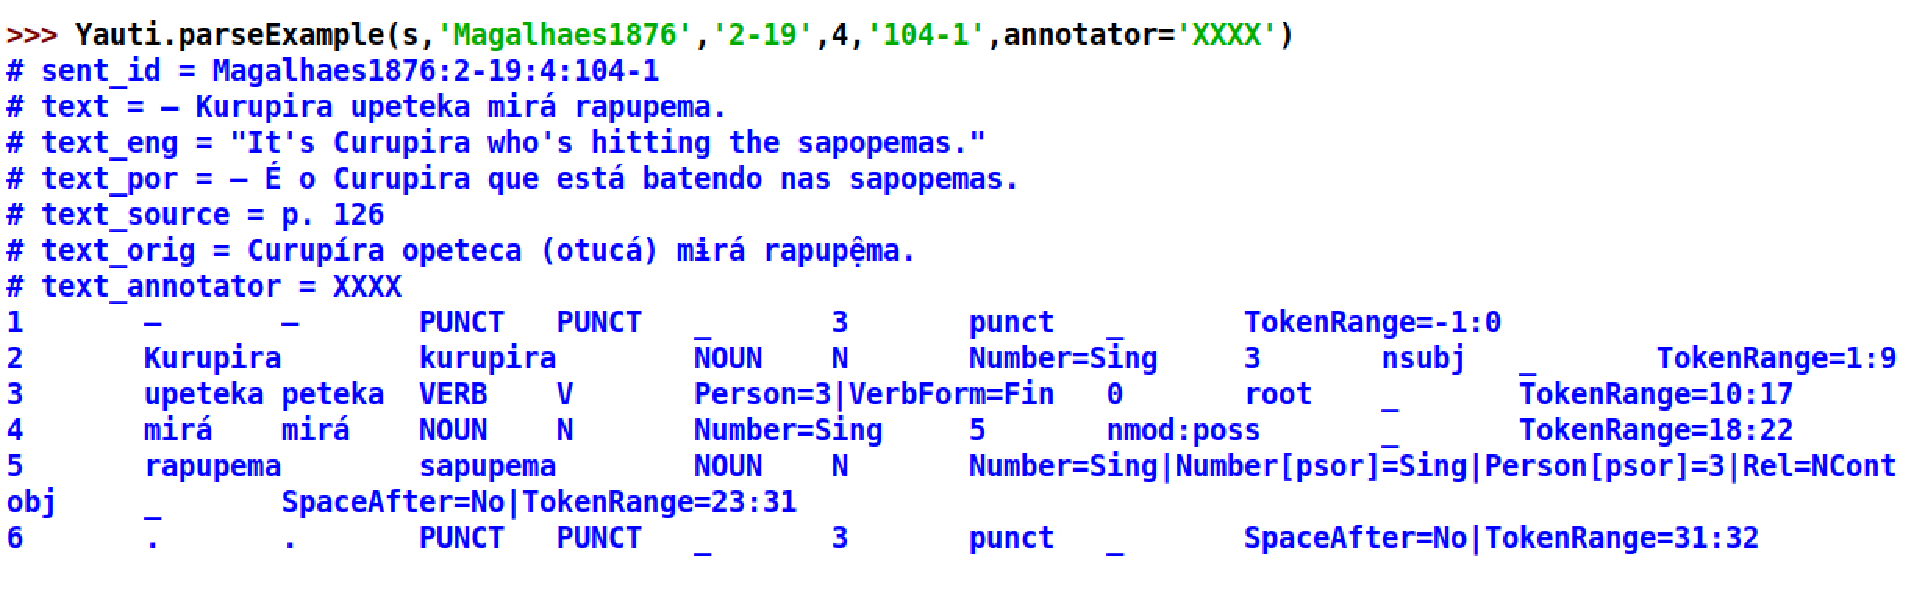
\includegraphics[width=\linewidth]{figures/upeteka-magalhaes-idle.pdf}
    \caption{Reaplicação da função \texttt{parseExample} sobre o exemplo de \textcite[p. 126]{magalhaes1876} após atualização do léxico da ferramenta.}
    \label{fig:upeteka-magalhaes-idle}
    \source{Elaboração própria.}
  \end{minipage}
\end{figure}

\begin{figure}[htbp]
  \centering
  \begin{minipage}{.75\textwidth}
    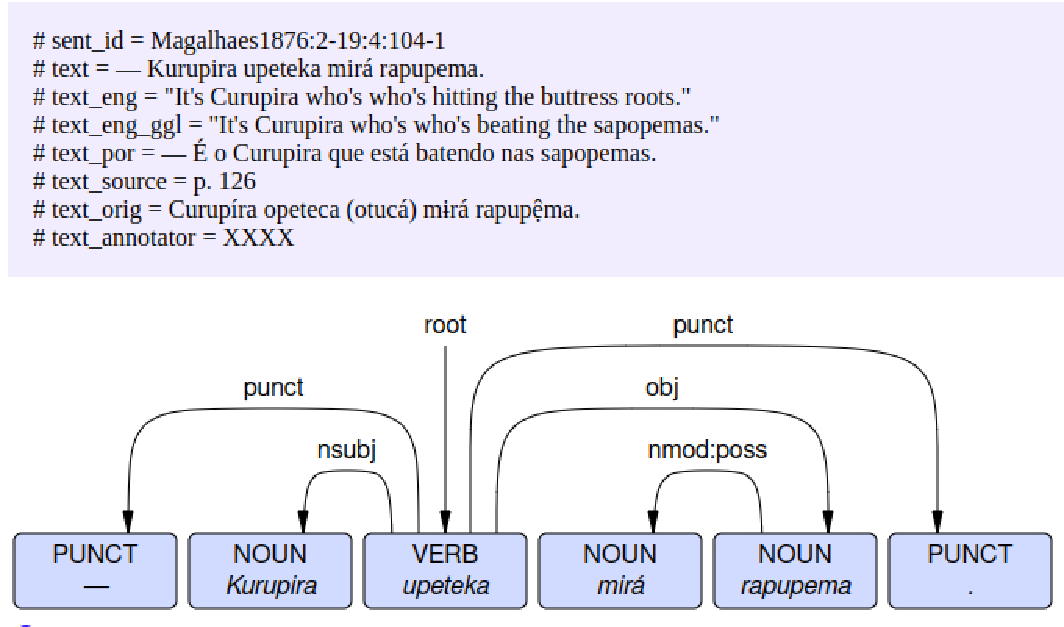
\includegraphics[width=\linewidth]{figures/upeteka-magalhaes-tree.pdf}
    \caption{Visualização da análise da Figura \ref{fig:upeteka-magalhaes-idle} com correção manual da tradução do português para o inglês realizada pelo tradutor do Google™.}
    \label{fig:upeteka-tree}
    \source{Elaboração própria.}
  \end{minipage}
\end{figure}

A Figura \ref{fig:sufixo-privativo-idle} exemplifica um outro tipo de situação com que o anotador se depara nos passos 4 e 5. Processos produtivos de formação de palavras, abundantes em nheengatu \parencite{sympson1877,stradelli1929,cruz2011,navarro2016,avila2021}, propiciam a criação de novos lexemas a qualquer momento. Entre esses mecanismos, destacam-se a reduplicação e a sufixação. Enquanto várias dessas formações se lexicalizaram e estão consignadas em \textcite{avila2021}, como \wt{purapuranga}{muito bonito}, reduplicação parcial de \wt{puranga}{bonito}, e \wt{sesaíma}{cego}, derivada de \wt{sesá}{olho} por meio do sufixo privativo \wt{ima}{sem}, encontramos nos textos outras derivações ainda não lexicalizadas, como \wt{paya-ima}{sem pai} (Figura \ref{fig:sufixo-privativo-idle}).\footnote{Em \textcite[p. 276]{stradelli1929} constam \say{paiay[m]a} e \say{maiayma} como acepções de \textit{órfão de pai} e \textit{órfão de mãe}.} Isso significa que apenas incorporar o inventário integral de lexemas de \textcite{avila2021} não permitiria a um analisador morfossintático automático reconhecer qualquer formação desse tipo. Para lidar com esses casos, o Yauti adota duas estratégias. Em casos completamente previsíveis como a reduplicação total, a ferramenta automaticamente identifica o processo derivacional, preenchendo o campo LEMMA com a base e o campo FEATS com o traço \texttt{Red=Yes} (Figura \ref{fig:utuka-tuka}). Noutros casos, exemplificado na Figura \ref{fig:sufixo-privativo-idle}, o anotador precisa inserir uma etiqueta especial prefixada por \texttt{/=} indicando o tipo de formação e a classe de palavra resultante, entre outras informações \pvtres. 

\begin{figure}[htbp]
  \centering
  \begin{minipage}{.75\textwidth}
    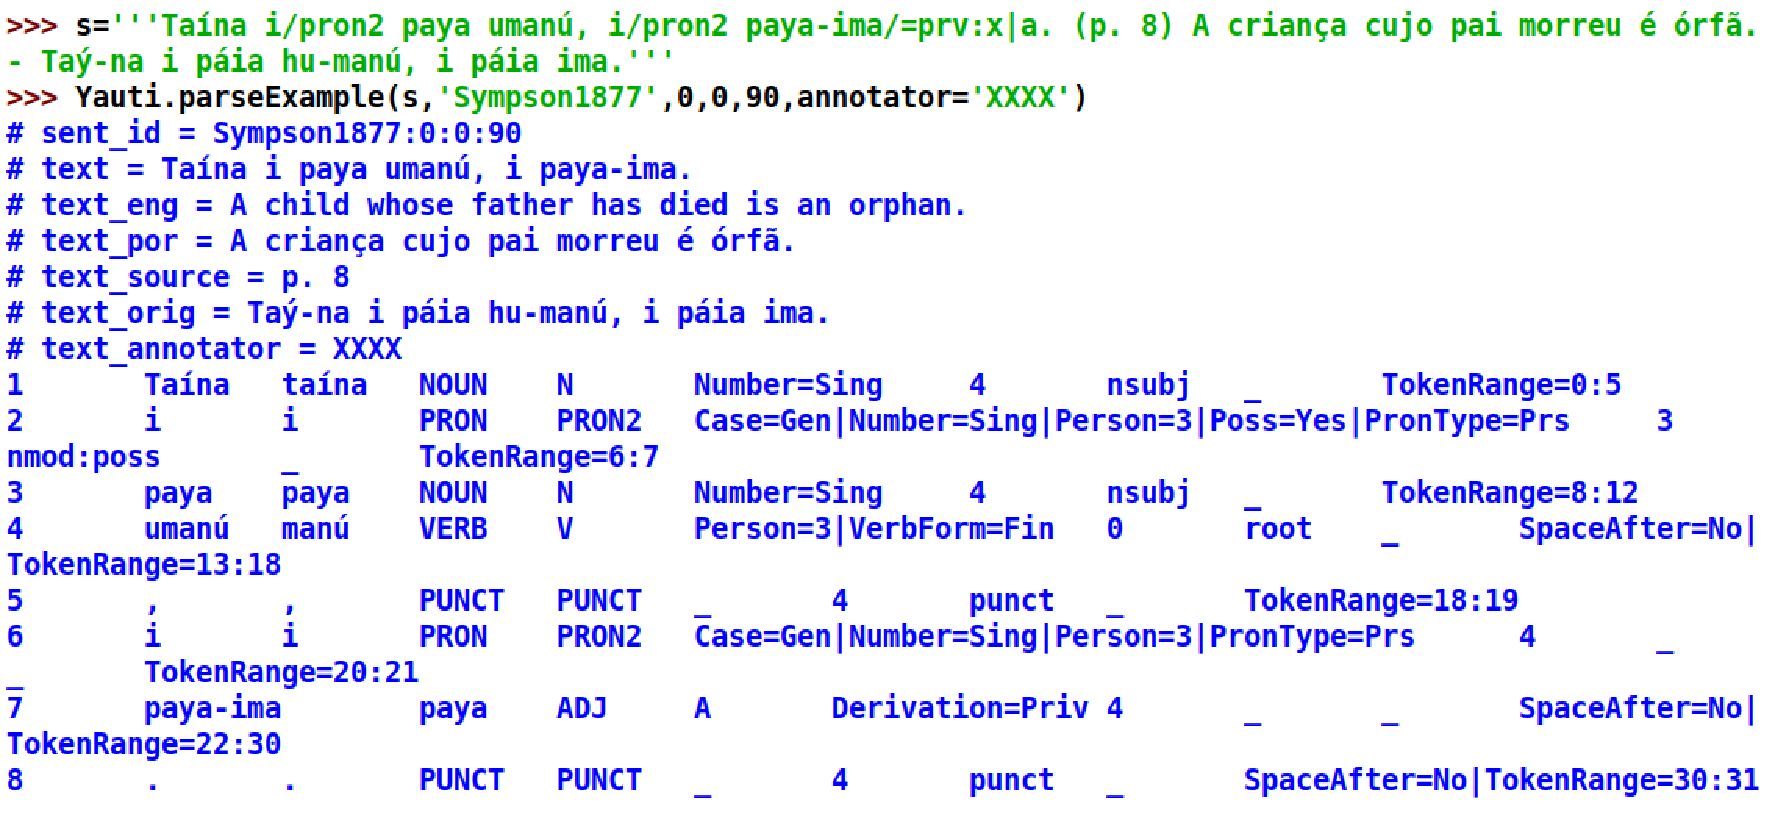
\includegraphics[width=\linewidth]{figures/sufixo-privativo-idle.pdf}
    \caption{Preparação de exemplo de \textcite[p. 8]{sympson1877} e primeira aplicação da função \texttt{parseExample} do Yauti.}
    \label{fig:sufixo-privativo-idle}
    \source{Elaboração própria.}
  \end{minipage}
\end{figure}

\begin{figure}[htbp]
  \centering
  \begin{minipage}{.75\textwidth}
    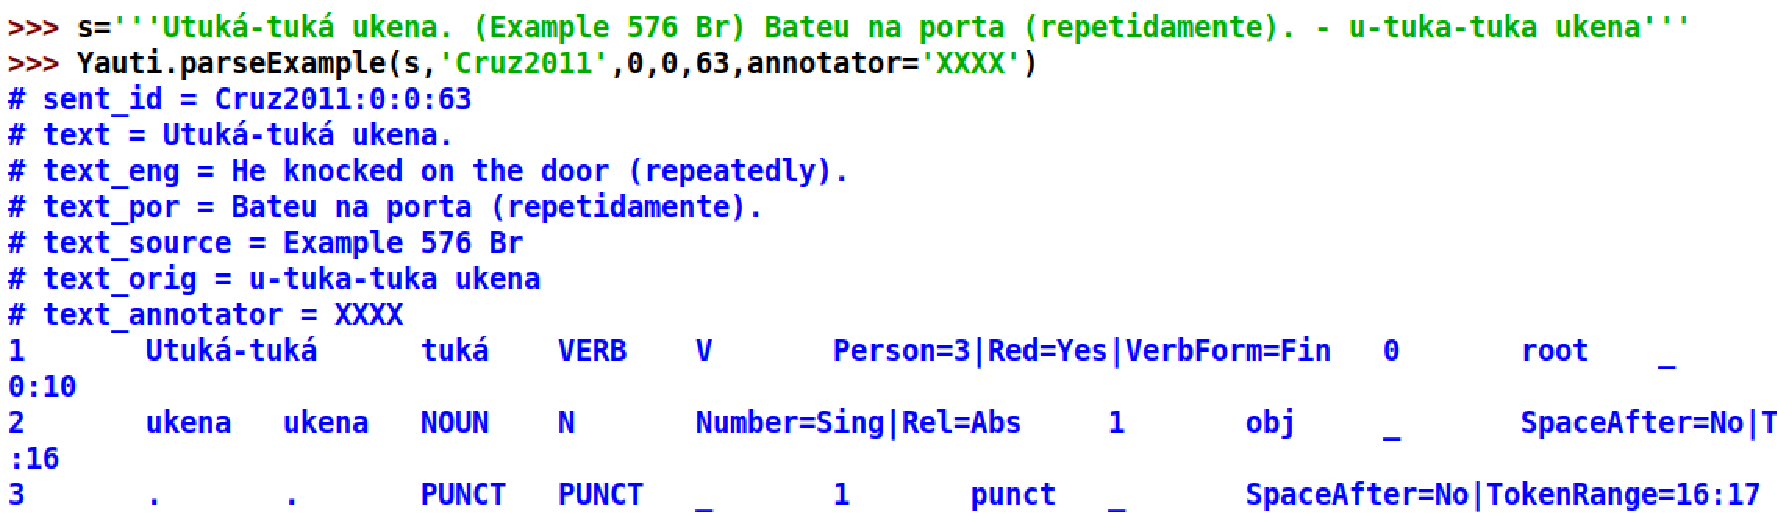
\includegraphics[width=\linewidth]{figures/utuka-tuka.pdf}
    \caption{Análise automática da reduplicação total pelo Yauti.}
    \label{fig:utuka-tuka}
    \source{Elaboração própria.}
  \end{minipage}
\end{figure}

Divergimos de \textcite{avila2021} em alguns aspectos relacionados à adaptação dos exemplos antigos, subtarefa do passo 2, adotando uma perspectiva mais conservadora, de modo a possibilitar investigações dialetológicas ou diacrônicas, preservando, via de regra, a pontuação\footnote{Maiusculizamos a primeira letra de sentenças e inserimos a pontuação final faltante, entre outras intervenções mínimas em casos de lapsos ou erros tipográficos óbvios.} e escolhendo, para cada palavra, a variante histórica mais próxima da forma original, sem inserir nem suprimir palavras, mesmo quando justificável sob a ótica do nheengatu rio-negrino atual. 

Comparem-se, na Figura \ref{fig:rodrigues-avila}, o texto original \texttt{text\_orig} de \textcite{rodrigues1890}, sem o relativizador \textit{waá}, com o texto secundário \texttt{text\_sec} de \textcite{avila2021} com esse subordinador. O atributo \texttt{cross\_reference} remete ao exemplo do \tbc~com a versão de \textcite{avila2021}, que também lematiza \wt{muirá}{árvore} como \textit{mirá} e separa com uma vírgula a última oração da sentença. Pelo contrário, limitamos nossas intervenções ao plano ortográfico, mantendo a forma \textit{muirá}, consignada em \textcite{avila2021} como variante histórica.

\begin{figure}[htbp]
  \centering
  \begin{minipage}{.75\textwidth}
    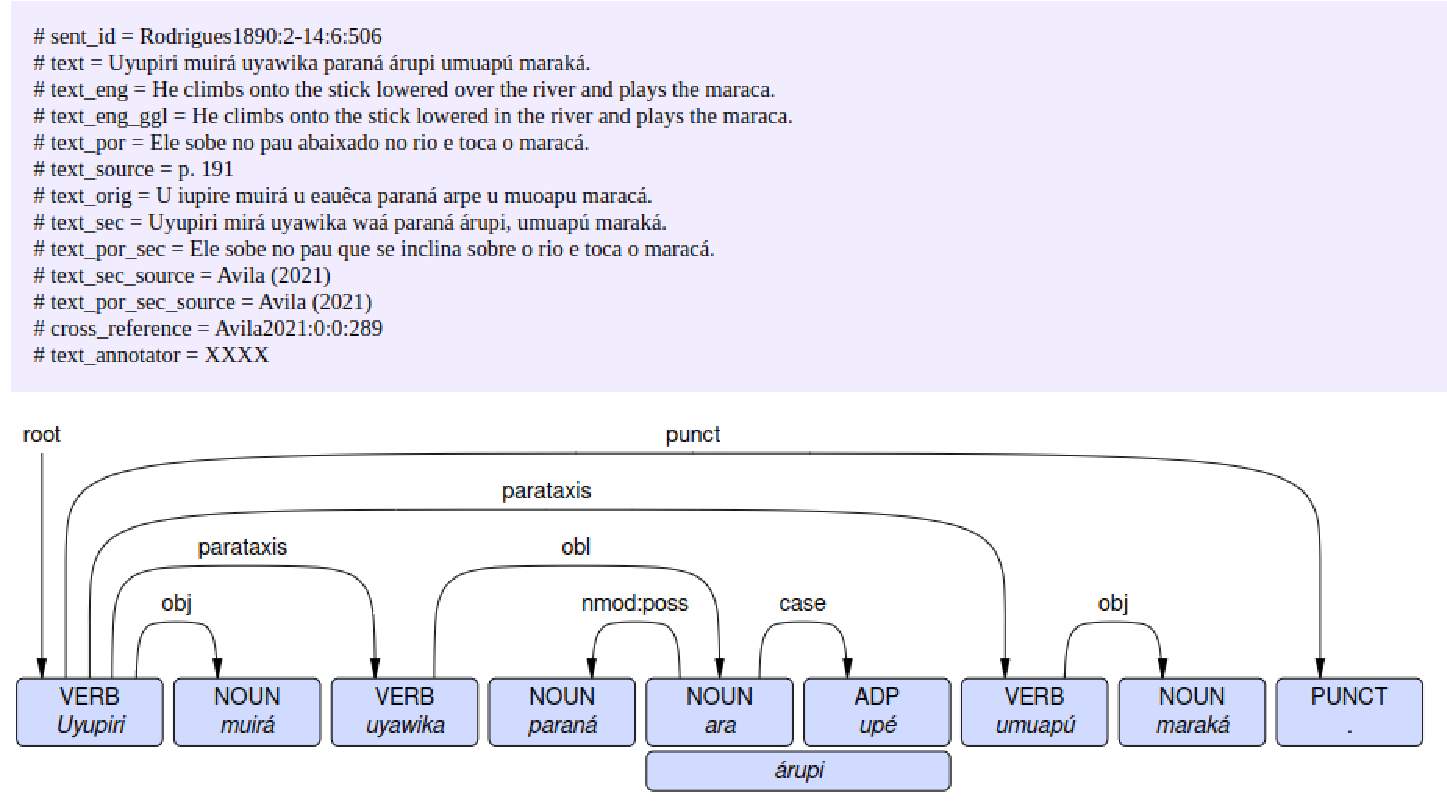
\includegraphics[width=\linewidth]{figures/rodrigues-avila.pdf}
    \caption{Comparação entre a adaptação textual do \tbc~e de \textcite{avila2021}.}
    \label{fig:rodrigues-avila}
    \source{Elaboração própria.}
  \end{minipage}
\end{figure}

Assinalamos determinadas idiossincrasias dos textos históricos com os traços \texttt{Style=\allowbreak Arch} e \texttt{Style=\allowbreak Rare}, indicando, no campo MISC, a forma canônica, como na Figura \ref{fig:style-arch}, na esteira de alguns \tbs~da \udc. Recorremos a essa estratégia, por exemplo, na anotação de sentenças com pronomes de segunda classe na função de objeto de um verbo sem marca de flexão, fenômeno que \textcite{avila2021} preserva nas suas abonações (Figura \ref{fig:style-arch}). No momento, o Yauti analisa esses pronomes, nessa configuração, erroneamente como sujeitos do verbo subsequente. Outras particularidades gramaticais do nheengatu do século XIX registradas nos exemplos de \textcite{avila2021}, como o prefixo \textit{e} de imperativo de segunda pessoa do singular e o dativo dos pronomes pessoais, são analisadas automaticamente pelo Yauti. Esses últimos fenômenos não estão marcados no \tbc~com \texttt{Style=\allowbreak Arch}, decisão que talvez alteremos no futuro.  

\begin{figure}[htbp]
  \centering
  \begin{minipage}{.75\textwidth}
    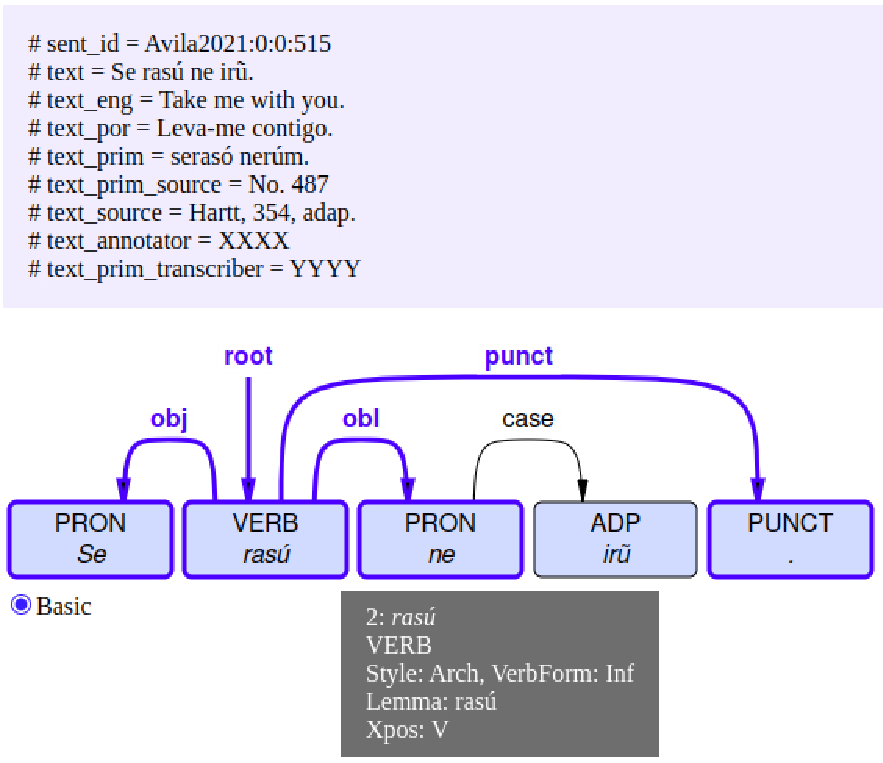
\includegraphics[width=\linewidth]{figures/style-arch.pdf}
    \caption{Exemplo com o traço \texttt{Style=Arch}.}
    \label{fig:style-arch}
    \source{Elaboração própria.}
  \end{minipage}
\end{figure}

Também discrepamos de \textcite{avila2021} ao seguirmos \textcite{cruz2011} na análise de formas como \wt{taumaã}{vêem} e \wt{tapurasí}{dançam} ao invés de desmembrá-las em \textit{ta umaã} e \textit{ta upurasí}, onde \textit{ta} constitui o pronome pessoal de terceira pessoa do plural. O Yauti trata \textit{tokens} desse tipo como formas do paradigma conjugacional, sem segmentá-los. No entanto, quando se depara com sequências do tipo de \textit{ta umaã}, preserva essa característica do texto, não realizando a junção do pronome e da forma verbal. 

\section{Aspectos da anotação}\label{sec:anotacao}
Esta seção aborda as principais decisões que nortearam a elaboração das representações no formato \conll~do \tbc, fornecendo também dados quantitativos nesse domínio. Começamos com a delimitação de sentenças e palavras, para em seguida tratar do preenchimento dos diferentes campos da tabela exemplificada na Figura \ref{fig:conllu}. Finalmente, apresentamos os resultados do \tbc~para as principais métricas de avaliação do projeto UD. 

\subsection{Segmentação sentencial e vocabular}\label{subsec:segmentacao}

Antes de proceder à anotação de textos conforme o modelo UD, cumpre determinar as unidades a serem anotadas. Na versão atual do \tbc, dois tipos de unidades são delimitadas: a sentença e a palavra sintática. O formato \conll~contempla também a segmentação dos textos em parágrafos, unidade que deixamos para incluir numa etapa futura. 

Por um lado, a marcação de parágrafos não é relevante para a anotação de grande parte dos materiais linguísticos do nheengatu, especialmente aqueles provenientes de exposições gramaticais, vocabulários e dicionários, como, por exemplo, \textcite{sympson1877} e \textcite{cruz2011}. Por outro lado, mesmo em narrativas comumente não se dividem os textos em parágrafos, como no caso das lendas coligidas por \textcite{Amorim1928} (Figuras \ref{fig:kukuhy-por} e \ref{fig:kukuhy-yrl}) e \textcite{casasnovas2006}. \textcite{magalhaes1876}, por sua vez, adota uma paragrafação irregular. Na lenda \textit{Como a noite apareceu}, constatamos indentações características de parágrafos, porém, essas marcas tipográficas parecem arbitrárias, não correspondendo aos parágrafos delimitados na tradução portuguesa. Enquanto na relativamente extensa lenda \textit{Jabuti e anta do mato} uma única indentação assinala o início do texto, na lenda \textit{O jabuti e a onça}, de menos de duas páginas, cada sentença é marcada por uma indentação.

\begin{figure}[htbp]
  \centering
  \begin{minipage}{.7\textwidth}
    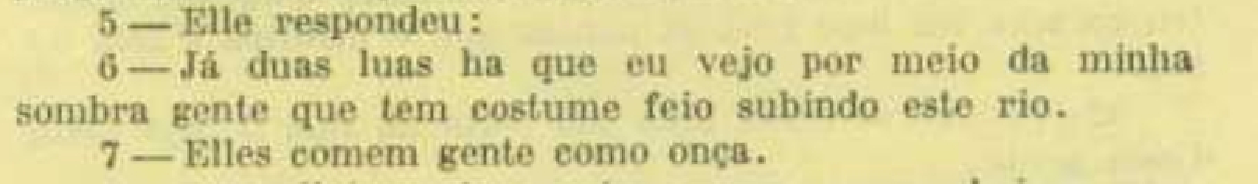
\includegraphics[width=\linewidth]{figures/Amorim-p301-por.pdf}
    \caption{Tradução de \textcite[p. 301]{Amorim1928} para o trecho da Figura \ref{fig:kukuhy-yrl}.}
    \label{fig:kukuhy-por}
    \source{Elaboração própria de recorte de página em PDF.}
  \end{minipage}
\end{figure}

\begin{figure}[htbp]
  \centering
  \begin{minipage}{.7\textwidth}
    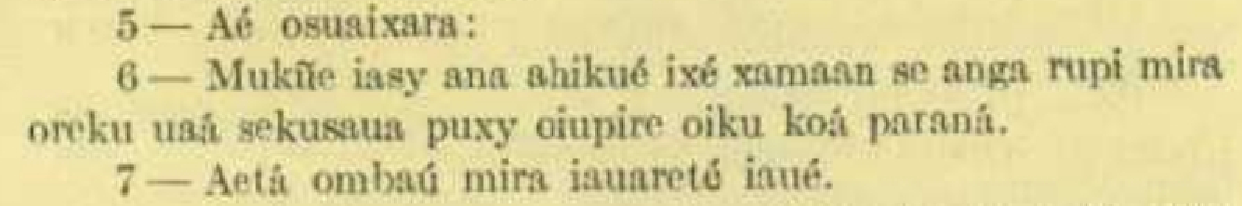
\includegraphics[width=\linewidth]{figures/Amorim-p309-yrl.pdf}
    \caption{Trecho da lenda \textit{Kukuhi} \parencite[p. 309]{Amorim1928}.}
    \label{fig:kukuhy-yrl}
    \source{Elaboração própria de recorte de página em PDF.}
  \end{minipage}
\end{figure}

Via de regra, consideramos sentenças individuais, nos textos em nheengatu, tanto as divisões de parágrafo delimitadas por pontuação final quanto segmentos numerados como o de número 7 da Figura \ref{fig:kukuhy-yrl}. Há casos, contudo, que discrepam dessa situação. Em narrativas, consideramos como partes de uma mesma sentença tanto a fala de personagem quanto o discurso, terminado por dois pontos, que a introduz, ainda que essas partes ocorram em parágrafos ou divisões numeradas distintas, como na Figura \ref{fig:kukuhy-yrl}. No \tbc, os segmentos cinco e seis constituem uma única sentença, a exemplo da sentença da Figura \ref{fig:aux-su}. 

A adoção desse critério de segmentação sentencial não é unânime nos \tbs~da coleção UD. Isso reflete-se na análise sintática da tradução em português, alemão ou inglês do exemplo da Figura \ref{fig:kukuhy-yrl} por meio do analisador sintático automático UDPipe 2. Quando se aplicam nessas traduções os modelos baseados nos \tbs~UD\_Portuguese-Bosque, UD\_German-GSD e UD\_English-Atis, todo o texto é tratado como uma única sentença, ao contrário do que ocorre no caso dos modelos treinados nos treebanks UD\_Portuguese-CINTIL, UD\_German-HDT e UD\_English-ParTUT, que dividem o texto em duas sentenças.

Em sentenças do tipo da Figura \ref{fig:kukuhy-yrl}, a segmentação (toquenização) vocabular constitui uma operação trivial: basta destacar das palavras os sinais de pontuação que as acompanham. Em diversas situações, porém, ocorre um descompasso entre as noções de palavra ortográfica, isto é, delimitada por espaço em branco ou sinal de pontuação, e de palavra sintática. Em nheengatu, esse é o caso, por exemplo, dos auxiliares incorporados (Figura \ref{fig:aux-incorp}) e de clíticos como o alomorfe monossilábico átono da partícula \textit{taá} de interrogativas parciais, o advérbio \wt{ntu}{somente} ou os alomorfes \textit{pe} e \textit{me} da adposição inessiva \wt{upé}{em} (Figuras \ref{fig:tata-pe-avila} e \ref{fig:paraname-avila}). 

\begin{figure}[htbp]
  \centering
  \begin{minipage}{.75\textwidth}
    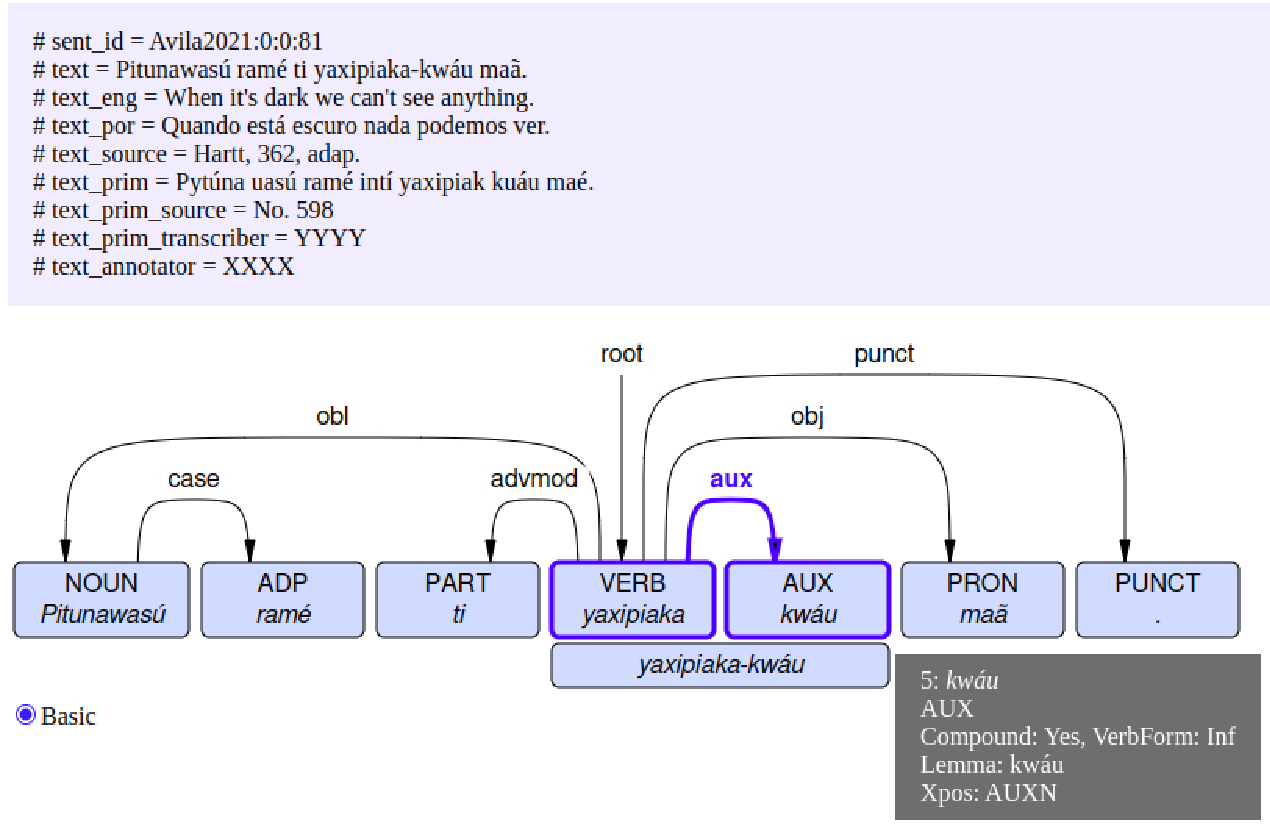
\includegraphics[width=\linewidth]{figures/aux-incorp.pdf}
    \caption{Anotação de auxiliar incorporado.}
    \label{fig:aux-incorp}
    \source{Elaboração própria.}
  \end{minipage}
\end{figure}

\begin{figure}[htbp]
  \centering
  \begin{minipage}{.75\textwidth}
    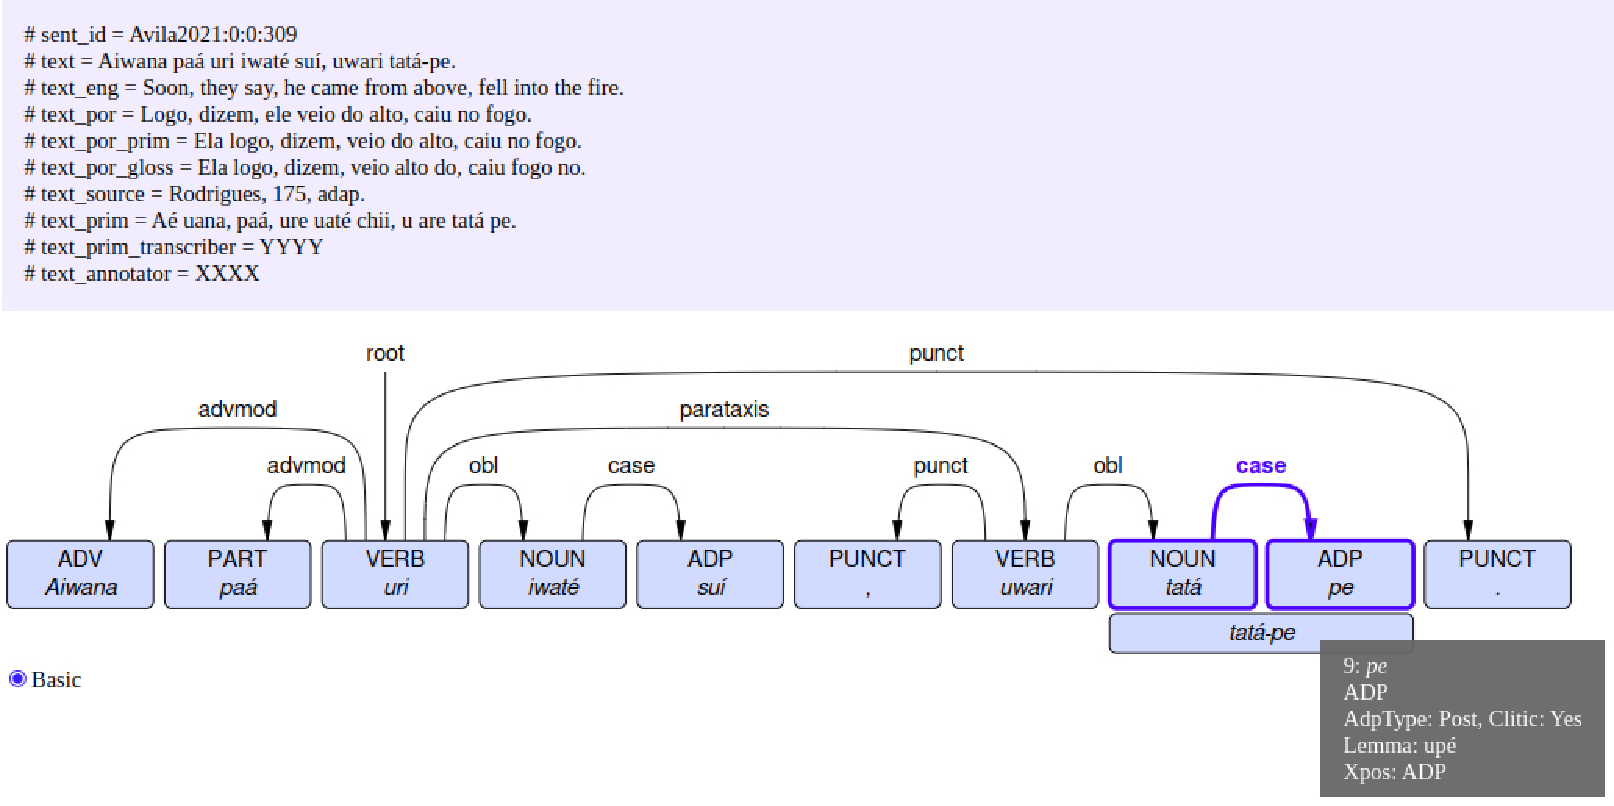
\includegraphics[width=\linewidth]{figures/tata-pe-avila.pdf}
    \caption{Anotação do alomorfe oral da posposição inessiva enclítica.}
    \label{fig:tata-pe-avila}
    \source{Elaboração própria.}
  \end{minipage}
\end{figure}

\begin{figure}[htbp]
  \centering
  \begin{minipage}{.75\textwidth}
    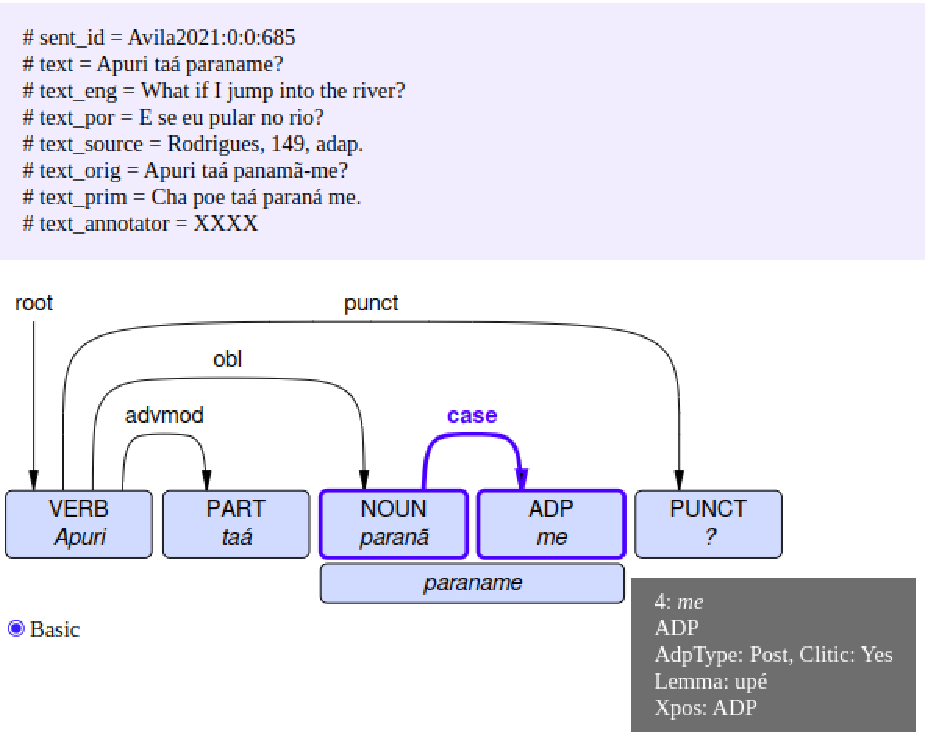
\includegraphics[width=\linewidth]{figures/paraname-avila.pdf}
    \caption{Anotação do alomorfe nasal da posposição inessiva enclítica.}
    \label{fig:paraname-avila}
    \source{Elaboração própria.}
  \end{minipage}
\end{figure}

A análise da Figura \ref{fig:tata-pe-avila} reflete a abordagem de \textcite[p. 588]{avila2021}, que considera \textit{pe} um alomorfe de \wt{upé}{em}, constituindo um clítico com verbete próprio de lema \textit{=pe}.\footnote{O sinal de igualdade indica a natureza clítica do morfema.} Ao nosso ver, essa análise estende-se naturalmente, no quadro de UD, ao exemplo da Figura \ref{fig:paraname-avila}. \textcite[p. 580]{avila2021}, pelo contrário, classifica \textit{paraname} como ``substantivo locativo'', equivalente a \textit{paranã upé} e traduzindo-se como \say{no rio}, constituindo a ``forma locativa'' de \wt{paraná}{rio}, lema com variante \textit{paranã}. No dicionário, \textit{paraná} e \textit{paraname} encabeçam verbetes principais, ao passo que \textit{paranã} constitui verbete que meramente remete a \textit{paraná}. Formas locativas análogas constituem verbetes de \textcite{avila2021}, como \wt{gantime}{na proa}, igualmente classificadas como substantivos locativos, classe que também engloba diversos lemas terminados em \textit{upi}, como \textit{árupi}, \textit{wírupi} e \textit{pitérupi}, formas locativas, respectivamente, de \wt{ara}{cima}, \wt{wira}{parte inferior} e \wt{pitera}{meio}. \textcite{navarro2016} classifica essas últimas formas como posposições, análise que inicialmente abraçamos, antes de adotarmos um tratamento consistente para todas as formas que \textcite{avila2021} considera substantivos locativos.  

\begin{figure}[htbp]
  \centering
  \begin{minipage}{.75\textwidth}
    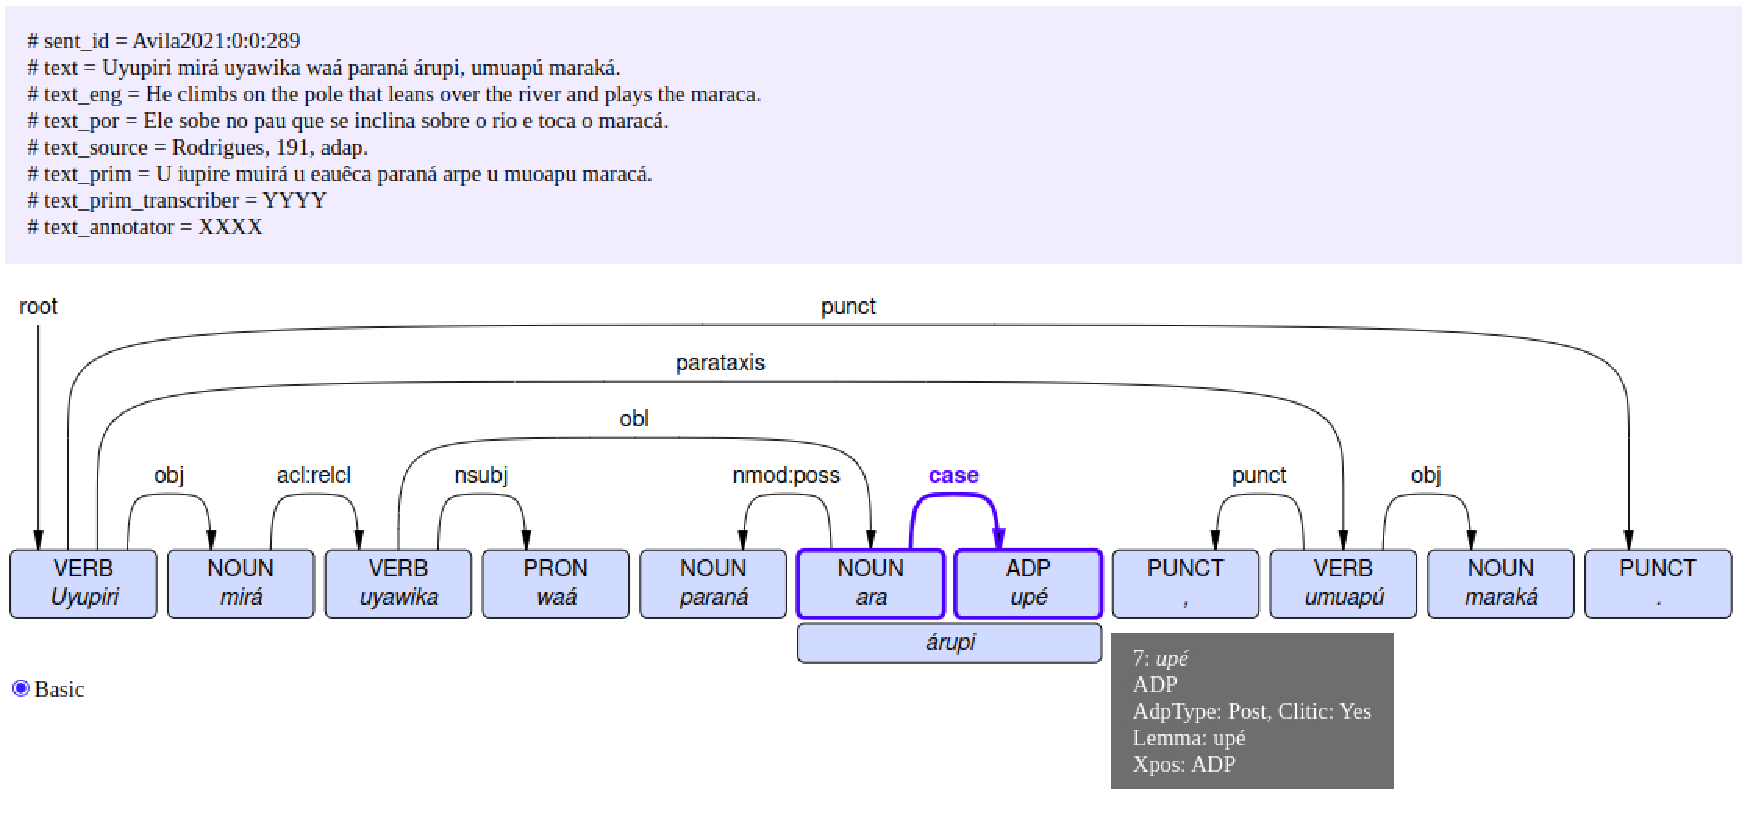
\includegraphics[width=\linewidth]{figures/arupi.pdf}
    \caption{Exemplo de anotação substantivo locativo.}
    \label{fig:arupi}
    \source{Elaboração própria.}
  \end{minipage}
\end{figure}

No modelo UD, palavras ortográficas que abrangem mais de uma palavra sintática, como nas Figuras \ref{fig:aux-incorp}, \ref{fig:tata-pe-avila}, \ref{fig:paraname-avila} e \ref{fig:arupi}, denominam-se palavras fusionadas, cujos componentes se ligam por hífen, conforme a ortografia de \textcite{avila2021}, apenas num subconjunto dos casos; comparem-se as Figuras \ref{fig:tata-pe-avila} e \ref{fig:paraname-avila}.  O Yauti identifica automaticamente os diferentes tipos de palavras fusionadas, segmentando e anotando os dois componentes, o segundo dos quais recebe o traço \texttt{Compound=Yes} ou \texttt{Clitic=Yes}, conforme se trata de composição (Figura \ref{fig:aux-incorp}) ou cliticização. Na anotação no formato \conll, uma palavra fusionada é assinalada na coluna 1 por um índice sob a forma de intervalo numérico \texttt{n-m}, em que \texttt{n} e \texttt{m} designam os índices da primeira e da última palavra sintática abrangida. Todos os campos da palavra fusionada são preenchidos por \texttt{—}, exceto o campo MISC. A anotação de uma palavra fusionada precede as anotações das palavras sintáticas que a integram.

\subsection{Lematização}\label{subsec:lematizacao}

Em línguas com morfologia flexional e derivacional como o nheengatu, o valor do campo LEMMA não coincide necessariamente com o campo FORM. Por exemplo, quando se trata de um substantivo uniforme no plural, ou seja, sufixado com \textit{-itá} (Figura \ref{fig:wira-miri-avila}), ou um verbo da série ativa conjugado (Figura \ref{fig:conllu}), o campo LEMMA abriga a forma de citação de dicionário, que, conforme \textcite{avila2021}, consiste no radical nominal e verbal, respectivamente, formas não marcadas de singular e infinitivo. 

\begin{figure}[htbp]
  \centering
  \begin{minipage}{.75\textwidth}
    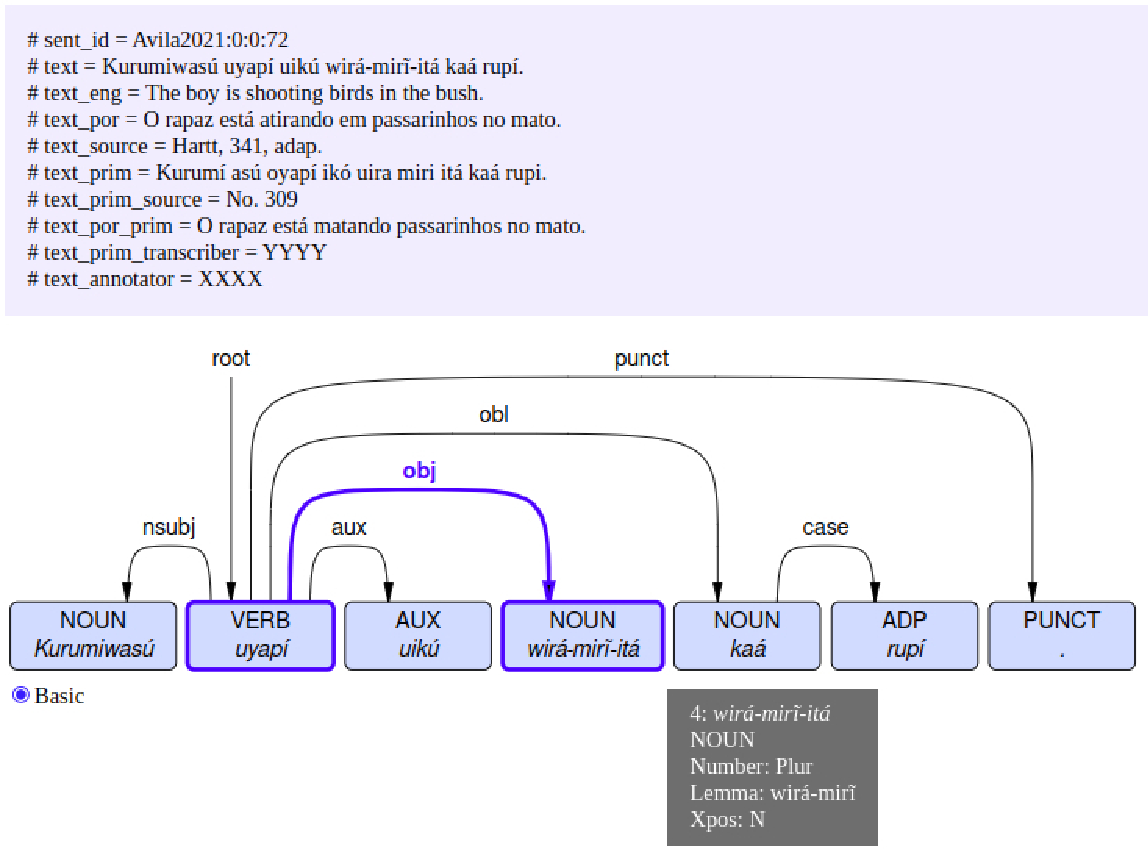
\includegraphics[width=\linewidth]{figures/wira-miri-avila.pdf}
    \caption{Lematização de substantivo uniforme no plural.}
    \label{fig:wira-miri-avila}
    \source{Elaboração própria.}
  \end{minipage}
\end{figure}

O prefixo \textit{yu-} de voz médio-passiva e os sufixos derivacionais modificadores, como os aspectuais, avaliativos, privativos ou de formação de coletivos, também são eliminados no processo de lematização. Nesses casos, as diferentes informações expressas por esses afixos são codificadas sob a forma de traços no campo FEATS (Figura \ref{fig:buyawasu}). De modo análogo procedemos com formas reduplicadas (Figura \ref{fig:redup}). 

\begin{figure}[htbp]
  \centering
  \begin{minipage}{.75\textwidth}
    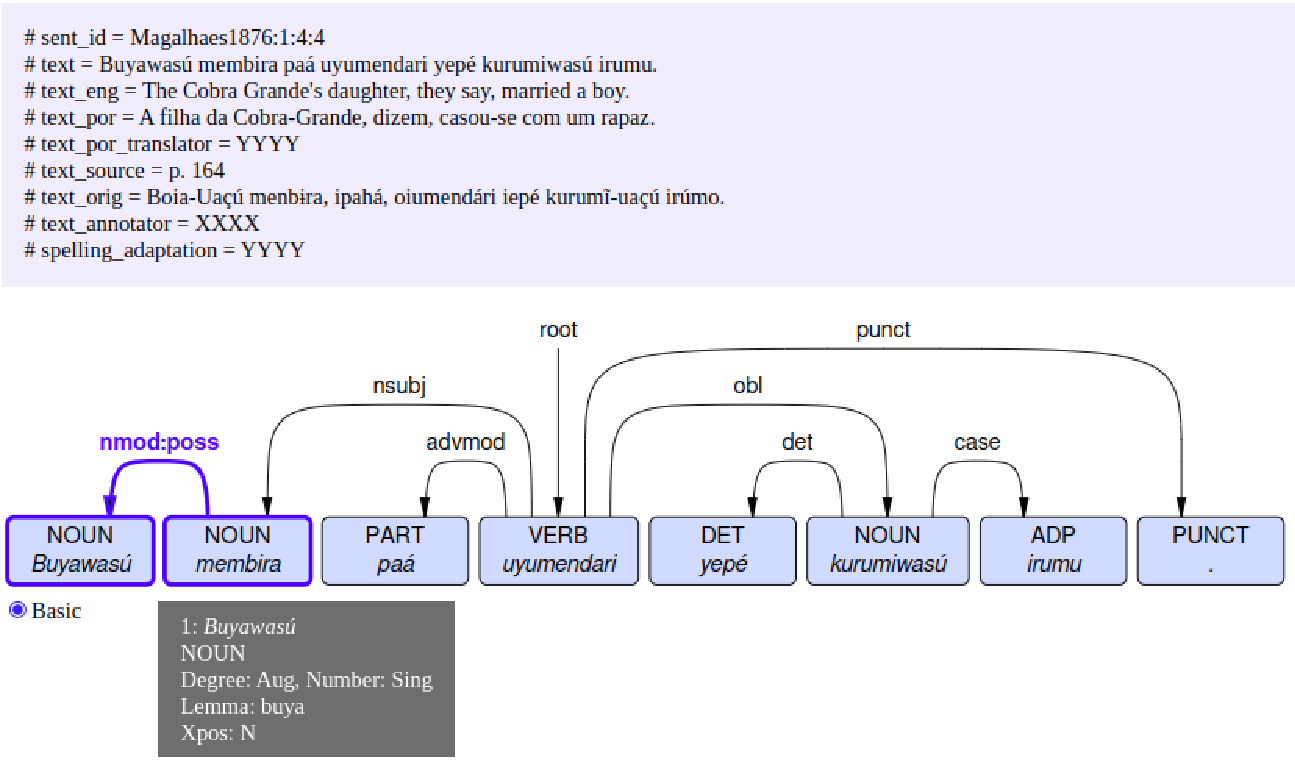
\includegraphics[width=\linewidth]{figures/buyawasu.pdf}
    \caption{Lematização de substantivo com sufixo aumentativo \textit{-wasú}.}
    \label{fig:buyawasu}
    \source{Elaboração própria.}
  \end{minipage}
\end{figure}

\begin{figure}[htbp]
  \centering
  \begin{minipage}{.75\textwidth}
    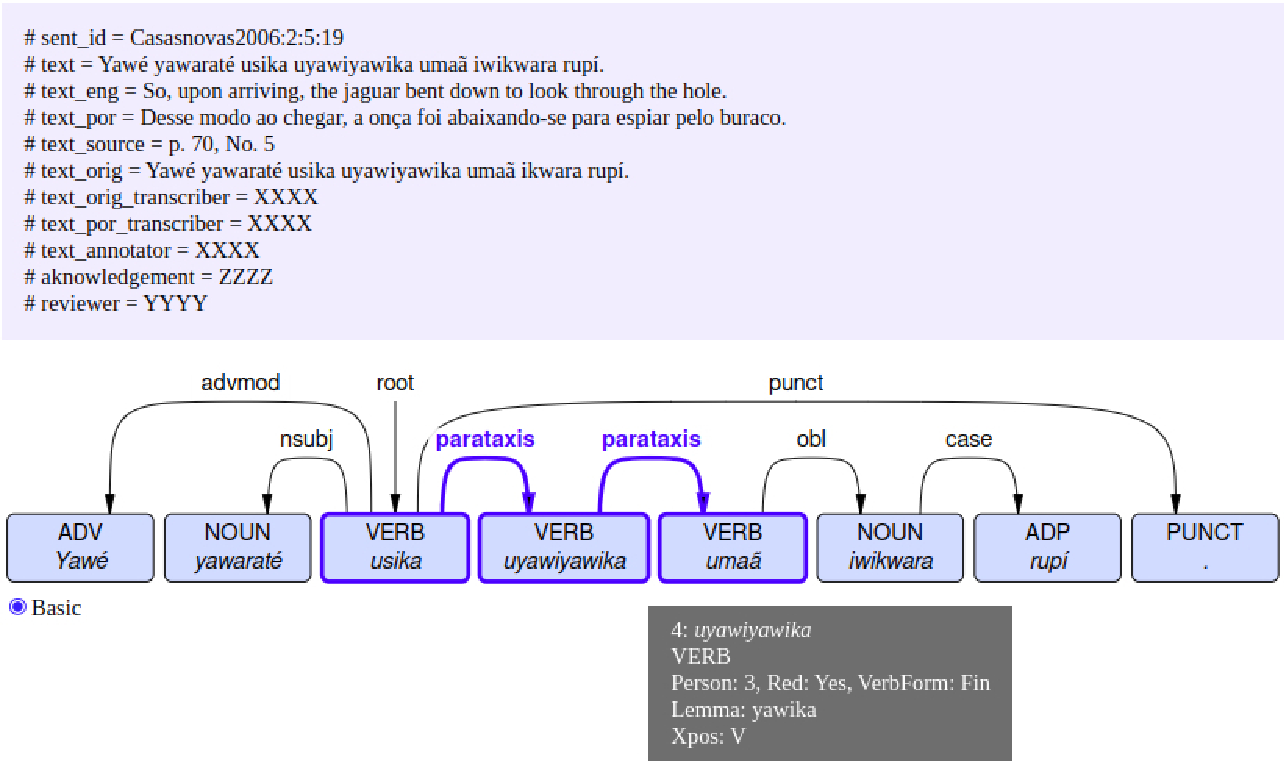
\includegraphics[width=\linewidth]{figures/redup.pdf}
    \caption{Lematização de verbo reduplicado.}
    \label{fig:redup}
    \source{Elaboração própria.}
  \end{minipage}
\end{figure}

O lema de formas lexicalizadas não composicionais, porém, preserva o afixo derivacional; comparem-se as formas \wt{buyawasú}{cobra grande} e \wt{kurumiwasú}{rapaz}, que lematizamos como \textit{buya} e \textit{kurumiwasú}, na esteira de \textcite{avila2021}. No \tbc, porém, nem sempre incluímos no campo LEMMA o lema da forma derivada de \textcite{avila2021}, preferindo a decomposição da forma quando composicional. Essa estratégia facilita o levantamento, no \tb, dos diferentes processos morfológicos que incidem sobre uma dada palavra, pois basta procurar pelo respectivo lema. Por exemplo, em \textcite{avila2021}, consta o verbete principal \textit{yumunhã}, parafraseado como \say{fazer-se; ser feito}, entre outras acepções. Em exemplos do \tb~com essa acepção, porém, o lema é \wt{munhã}{fazer}. Dado que lexicalização e composicionalidade são fenômenos graduais, é possível que decisões atuais no \tb~nesse domínio da lematização sejam revistas à luz de critérios que venham a ser definidos. 

De uma maneira geral, adotamos as decisões de lematização de \textcite{avila2021}. No entanto, em vez do radical das palavras com prefixos relacionais, preferimos acompanhar \textcite{navarro2016}, utilizando como lema a forma absoluta dos substantivos poliformes, v.g., \wt{tetama}{terra} com prefixo absolutivo \textit{t}, e a forma com prefixo de contiguidade \textit{r} de posposições e verbos de segunda classe, v.g., \wt{ruakí}{perto de} e \wt{rurí}{estar feliz}. Cremos que essa decisão se coaduna mais com o espírito lexicalista de UD. De fato, enquanto nos deparamos nos textos com formas como \textit{kwáu} (Figura \ref{fig:aux-incorp}) e \textit{sendú} (Figura \ref{fig:senu}), uma forma como \textit{urí} em vez de \textit{surí} ou \textit{rurí} não parece possível, pelo menos não encontramos registros em \textcite{avila2021}.

\begin{figure}[htbp]
  \centering
  \begin{minipage}{.75\textwidth}
    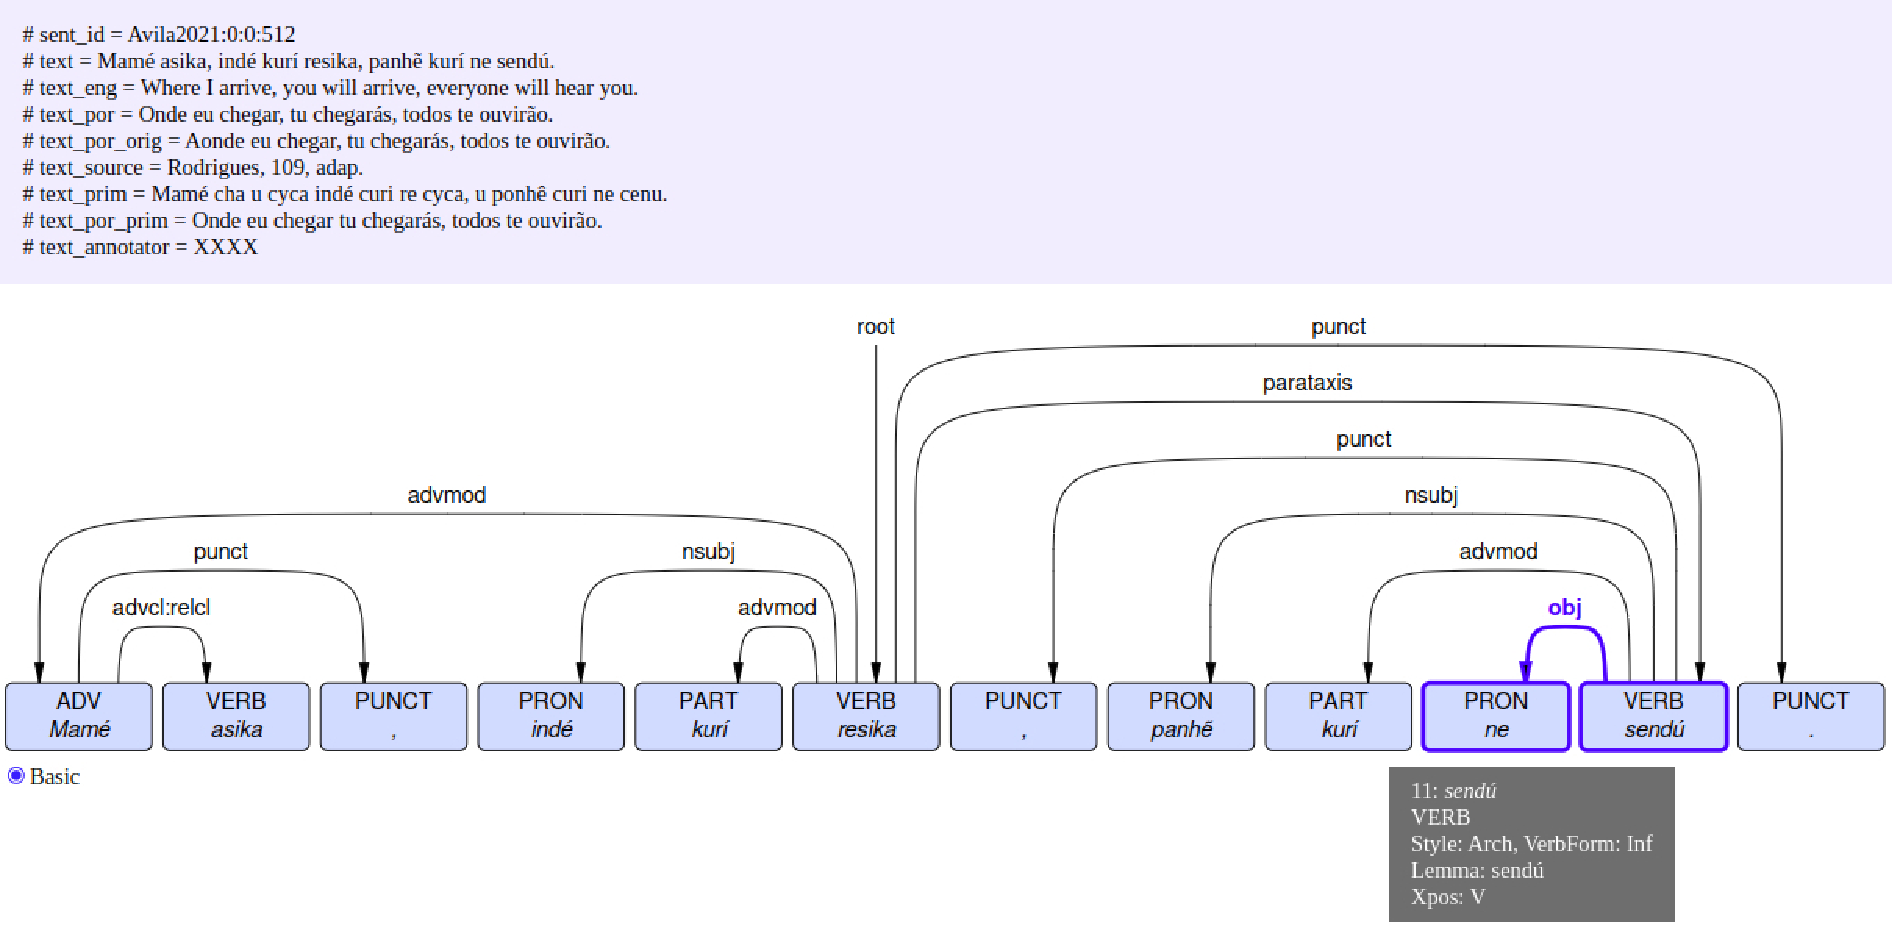
\includegraphics[width=\linewidth]{figures/senu.pdf}
    \caption{Exemplo com forma verbal no infinitivo.}
    \label{fig:senu}
    \source{Elaboração própria.}
  \end{minipage}
\end{figure}

\subsection{Classes de palavras, traços morfológicos e relações sintáticas}\label{classes}
Língua de gramática alheia a regulamentações oficiais, o nheengatu não dispõe de um inventário de classes de palavras normativo ou consensual. \textcite{sympson1877} e \textcite{moore-facundes-pires-1994} resumem o vocabulário da língua a conjuntos de sete e oito classes, respectivamente, cuja interseção se limita a cinco elementos. Faltam ao segundo conjunto as conjunções e \say{sinais} do primeiro, que, por sua vez, carece das partículas, pronomes e demonstrativos daquele, subsumidos noutras classes, como os adjetivos.\footnote{Na classe dos \say{sinais}, \textcite{sympson1877} abriga elementos heterogêneos como sufixos derivacionais, interjeições e partículas.} 

\textcite{cruz2011} propõe uma classificação hierárquica com diferentes classes e subclasses. Nesse sistema, as palavras da língua são agrupadas inicialmente em duas macroclasses, a saber, palavras lexicais e palavras gramaticais, perfazendo, ao todo, sete classes, das quais não constam os adjetivos, que inexistiriam no nheengatu. Integram a primeira macroclasse verbos, advérbios, posposições, \say{índices de pessoa} e nomes, os quais se dividem em substantivos e dêiticos, subclasse que abarca parte dos pronomes de outras abordagens. As palavras gramaticais classificam-se em partículas e clíticos, as primeiras englobando diferentes subclasses, como as conjunções, subordinadores, interjeições e mais de duas dezenas de subtipos de partículas, responsáveis pela expressão da interrogação, negação, tempo, aspecto, modo, modalidade 	\textit{etc.} Essa taxonomia não esgota o inventário terminológico de que \textcite{cruz2011} se vale para descrever as propriedades morfológicas e sintáticas das palavras nheengatus. Determinante, (artigo) indefinido, (verbo) auxiliar, quantificador e numeral são algumas das outras classes a que se refere, a última das quais sugere integrar a classe dos nomes.  

A proposta de \textcite{cruz2011} difere em pontos essenciais da abordagem do modelo UD (\Cref{tab:upos}). Nessa teoria, a distinção entre clíticos e não clíticos é ortogonal à classificação de palavras, que também não comporta os \say{índices de pessoa} de \textcite{cruz2011}, prefixos de nível subpalavra. Desse modo, no \tbc, assinalamos com o traço \texttt{Clitic=Yes} posposições, advérbios e partículas clíticas. Por outro lado, elementos classificados como morfemas flexionais, como os prefixos da série ativa, não constituem, no \tb, nós nas árvores sintáticas. Outra diferença refere-se à análise das partículas, que, conforme a \Cref{tab:upos}, constitui classe disjunta de conjunções e interjeições. Finalmente, as classes determinante, pronome e numeral de UD não possuem correlatos diretos na proposta de \textcite{cruz2011}. 

\textcite{avila2021}, pelo contrário, opera, na seção \textit{categoria gramatical} da microestrutura dos verbetes do dicionário, com uma classificação em linhas gerais mais próxima das duas primeiras colunas da \Cref{tab:upos}, das quais discrepa pela ausência das classes auxiliar e determinante e não distinção entre conjunções coordenativas e subordinativas. Na exposição gramatical que precede os verbetes do dicionário, contudo, \textcite{avila2021} identifica diversos tipos de subordinadores. Por outro lado, no corpo das acepções dos verbos \textit{ikú} e \textit{mupika}, refere-se ao emprego deles como auxiliares. A distinção entre determinantes e pronomes da \Cref{tab:upos} corresponde, em linhas gerias, aos rótulos pronomes substantivos e pronomes adjetivos de \textcite{avila2021}. \textcite{avila2021}, na trilha de \textcite{moore-facundes-pires-1994}, entre outros, defende a existência de adjetivos em nheengatu. 

A Figura \ref{fig:treebank-stats} permite comparar as quantidades de etiquetas de classes de palavras, traços morfológicos e relações de dependência do \tbc~com as dos cinco \textit{corpora} que o seguem na lista dos seis maiores \tbs~de línguas ameríndias da \udc. Abstraindo da etiqueta \texttt{X}, inusada no \tbc~e no UD\_Kiche-IU, e de \texttt{ADJ} e \texttt{PART}, inexistentes, respectivamente, no UD\_Guajajara-TuDeT e nos \tbs~do Nahuatl, os cinco \textit{corpora} compartilham o mesmo subconjunto das etiquetas da \Cref{tab:upos}, do qual apenas \texttt{SYM} não ocorre. Nas duas outras dimensões, o \tbc~iguala ou supera os demais \tbs. Ao todo, o \tbc~contém 36 relações sintáticas, das quais três são subtipadas, e 76 combinações diferentes de atributos e valores, fazendo jus à riqueza gramatical do nheengatu.    

\begin{figure}[htbp]
  \centering
  \begin{minipage}{.75\textwidth}
    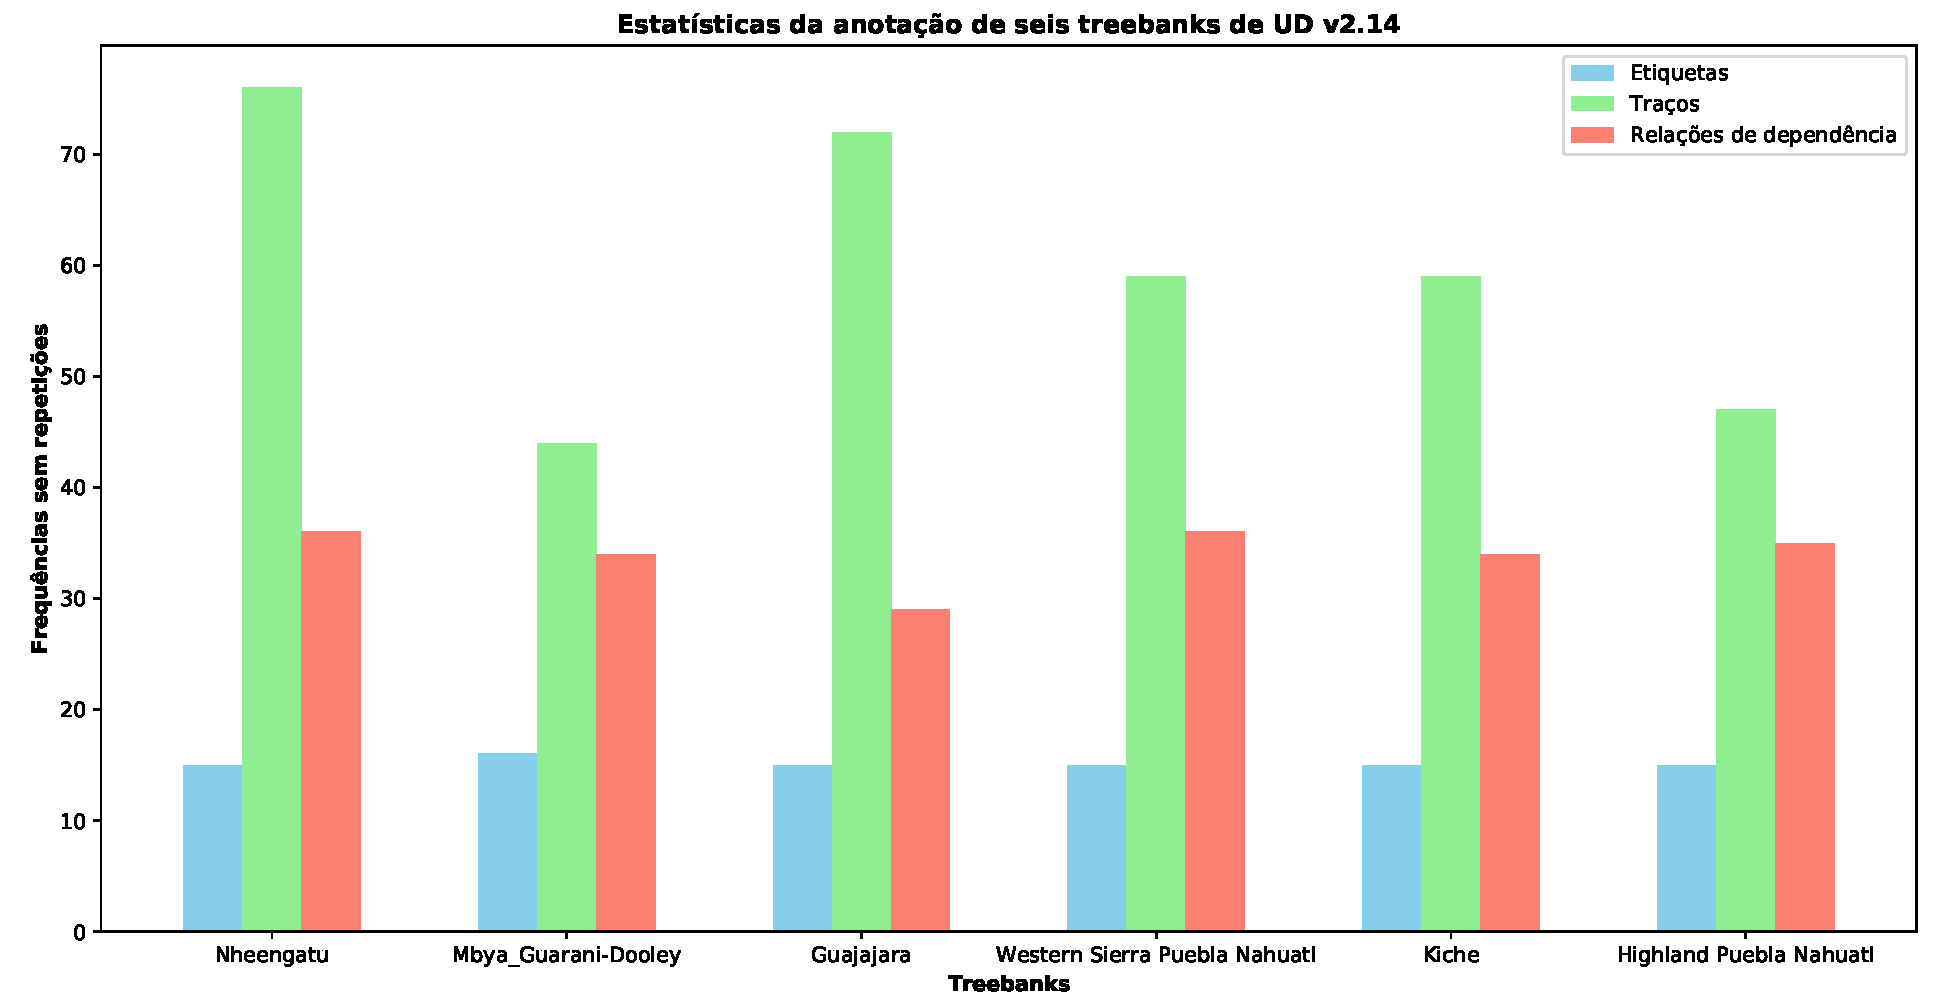
\includegraphics[width=\linewidth]{figures/TreebankStats6TBs.pdf}
    \caption{Quantidade sem repetições de etiquetas de classes de palavras, traços morfológicos e relações de dependência dos seis maiores \tbs~de línguas ameríndias da versão v2.14. da \udc.}
    \label{fig:treebank-stats}
    \source{Elaboração própria com base nos dados de \textcite{zeman2024universal}.}
  \end{minipage}
\end{figure}

A Figura \ref{fig:tag-freq} exibe as frequências absolutas das etiquetas de classes de palavras dos três maiores \tbs~de línguas indígenas sul-americanas e do maior de língua indígena norte-americana na \udc. O \tbc~ocupa a primeira ou segunda posição na quantidade de 11 das 16 etiquetas do seu conjunto de partes do discurso. A Figura \ref{fig:rel-tag-freq} contrasta os três maiores \tbs~de línguas indígenas brasileiras com o maior de língua portuguesa quanto às frequências relativas dessas etiquetas. Constatamos nos dois gráficos que o \tbc~possui um número razoável de ocorrências mesmo daquelas classes de palavras menos frequentes, como \texttt{CCONJ}, \texttt{NUM} e \texttt{INTJ}, diferentemente de outros \tbs~de línguas indígenas e mesmo do UD\_Portuguese-CINTIL, com uma frequência relativa de \texttt{INTJ} tão baixa que nem aparece na Figura \ref{fig:rel-tag-freq}, não obstante o quase meio milhão de palavras desse \tb. 

\begin{figure}[htbp]
  \centering
  \begin{minipage}{.75\textwidth}
    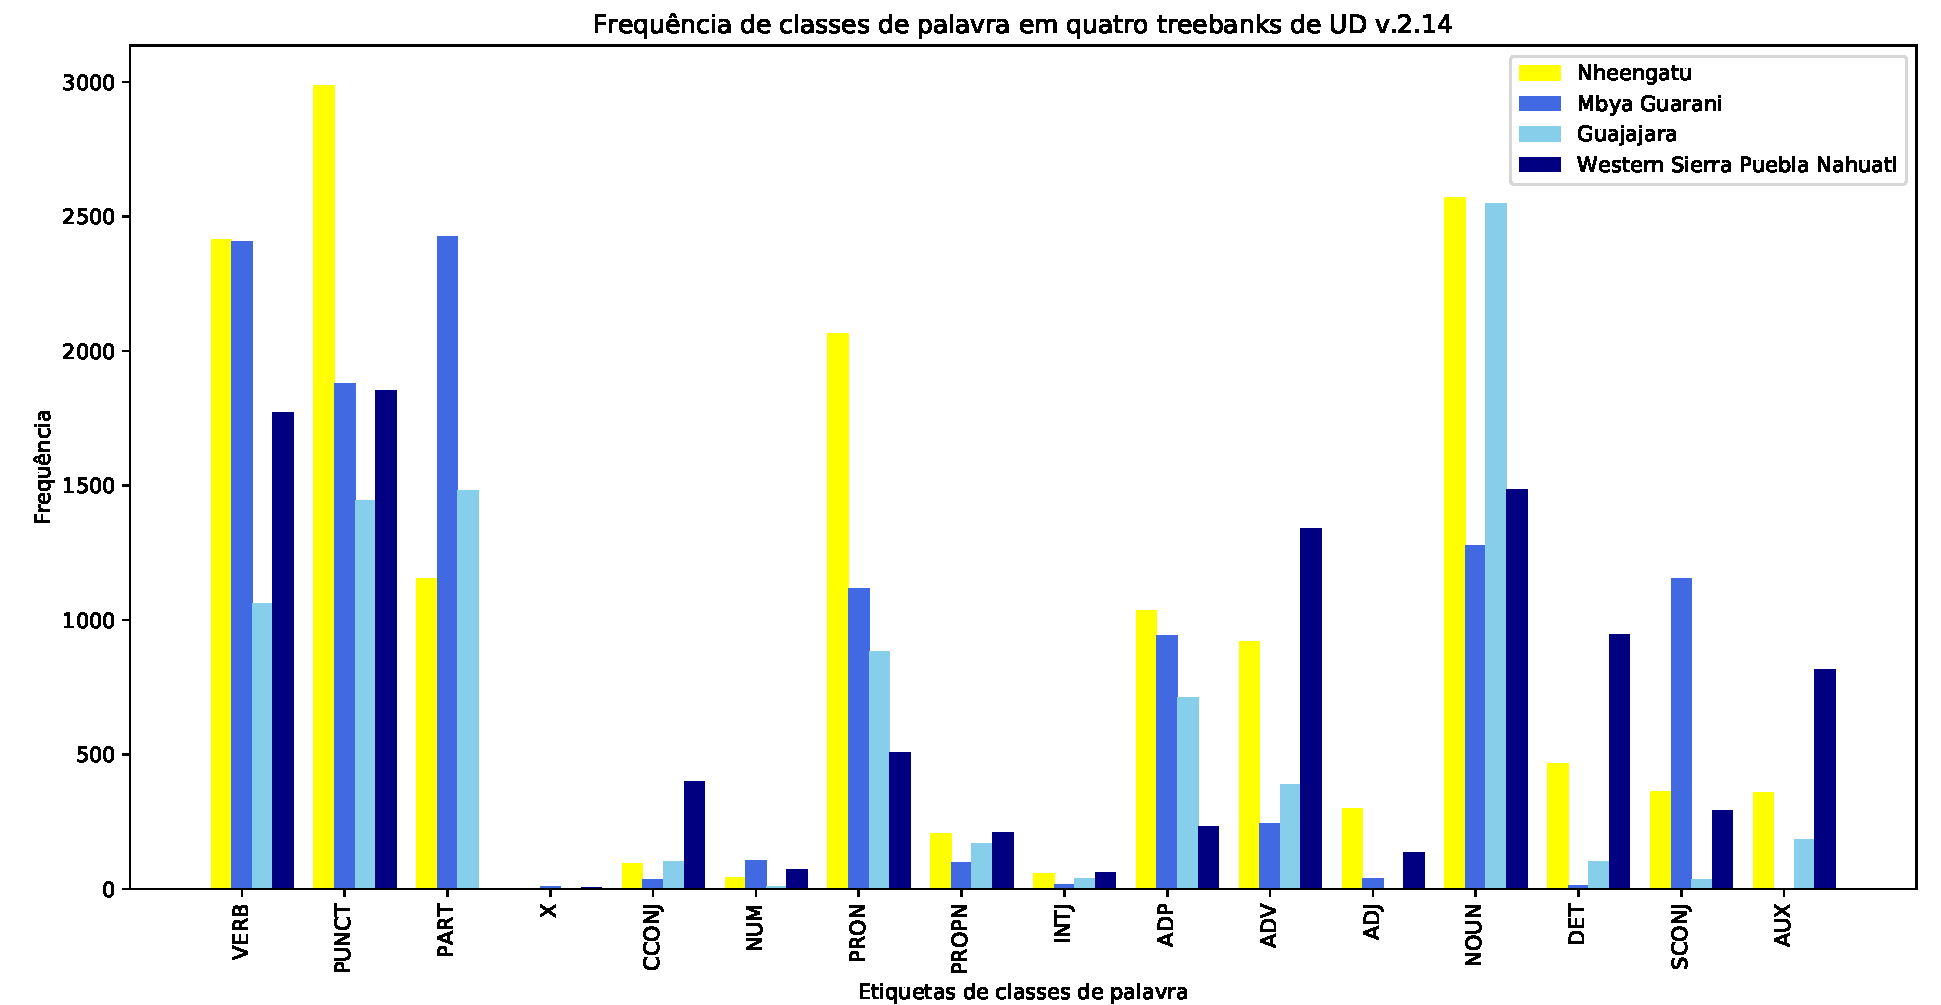
\includegraphics[width=\linewidth]{figures/TagFreq4TBs.pdf}
    \caption{Classes de palavra em quatro \tbs~de línguas ameríndias na \udc.}
    \label{fig:tag-freq}
    \source{Elaboração própria com base nos dados de \textcite{zeman2024universal}.}
  \end{minipage}
\end{figure}

\begin{figure}[htbp]
  \centering
  \begin{minipage}{.75\textwidth}
    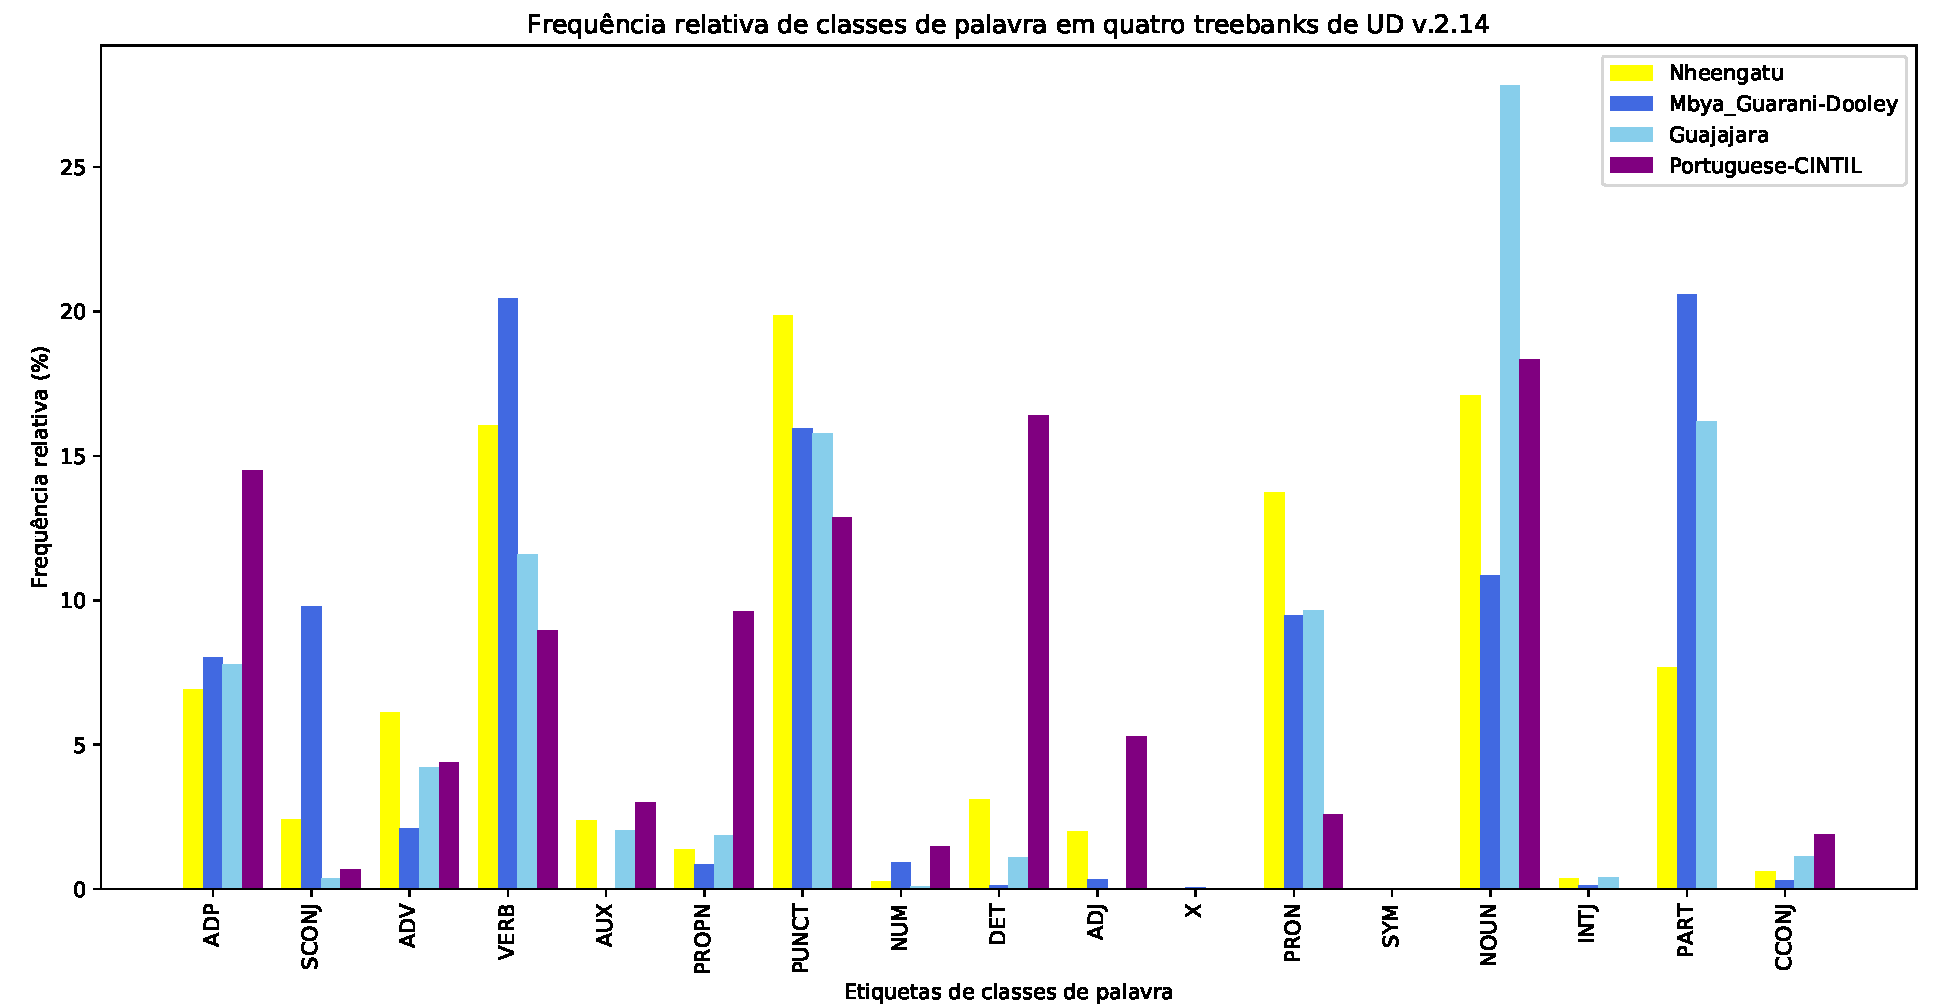
\includegraphics[width=\linewidth]{figures/RelTagFreq4TBsCINTIL.pdf}
    \caption{Frequências relativas das etiquetas de classe de palavra dos três maiores \tbs~de línguas indígenas brasileiras e do maior de língua portuguesa na \udc.}
    \label{fig:rel-tag-freq}
    \source{Elaboração própria com base nos dados de \textcite{zeman2024universal}.}
  \end{minipage}
\end{figure}

\subsection{Avaliação}\label{avaliacao}
Atualmente, o \textit{script} \href{https://github.com/UniversalDependencies/tools/blob/master/validate.py}{validate.py} sanciona integralmente todas as 1.470 sentenças do \tbc, a anotação de 28.37\% das quais foram revistas por um ou dois revisores. Esse \textit{script} constitui o principal crivo para admitir ou rejeitar um \tb~numa \textit{release} da \udc, servindo também para situar os \tbs~em diferentes faixas de validade. O \tbc~atualmente integra o grupo de 168 \tbs~(59,36\% de 283) de um total de 118 línguas (73,29\% de 161) com o status \texttt{CURRENT VALID}, o mais alto. 

O \textit{script} \href{https://github.com/UniversalDependencies/tools/blob/master/validate.py}{validate.py}, porém, não é abrangente o suficiente para detectar problemas de anotação específicos de uma língua particular ou mesmo análises que parecem implausíveis em qualquer língua, como um verbo regendo dois objetos diretos. Para assegurar uma maior qualidade de anotação, os \tbs~são submetidos também ao Udapi \parencite{popel-etal-2017-udapi-k}, um \textit{framework} que, entre outras funcionalidades, gera, para um dado \tb, um relatório de erros de anotação, como, por exemplo, múltiplos objetos diretos. No exemplo da Figura \ref{fig:erro-udapi}, o Udapi indica que as formas verbais finitas da sentença carecem de indicação de modo verbal. É questionável, porém, se isso realmente constitui erro, uma vez que, no nheengatu, o modo verbal, quando não subentendido, é normalmente indicado por meio de partículas.

\begin{figure}[htbp]
  \centering
  \begin{minipage}{.9\textwidth}
    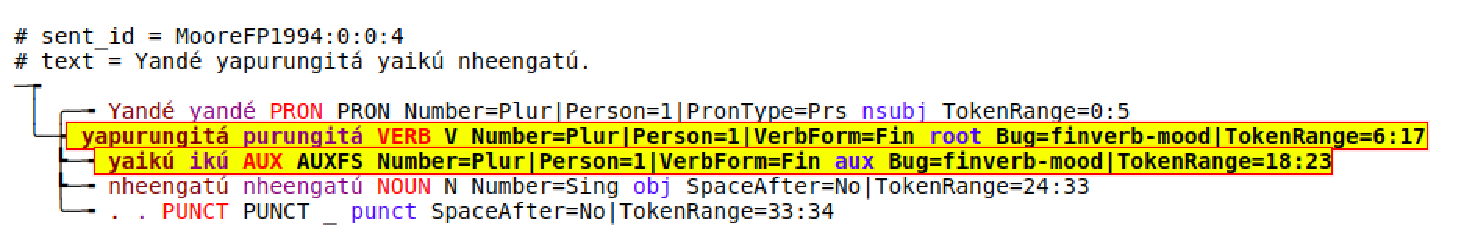
\includegraphics[width=\linewidth]{figures/erro-udapi.pdf}
    \caption{Relatório de erros de anotação gerado pelo comando \texttt{udapy -HAM ud.MarkBugs} para a sentença da Figura \ref{fig:conllu}. Os erros são assinalados pela palavra \textit{Bug}, seguida de uma abreviatura que identifica o tipo de erro.}
    \label{fig:erro-udapi}
    \source{Elaboração própria.}
  \end{minipage}
\end{figure}

O Udapi computa 2.726 erros de anotação para o \tbc, 2.580 dos quais são do tipo exemplificado na Figura \ref{fig:erro-udapi}. A abreviatura \texttt{fin-verb-mood} indica que a forma verbal finita carece de especificação de modo verbal. A quantidade desses erros compõe com uma série de outros parâmetros um cálculo, registrado no arquivo \texttt{eval.log} do ramo mestre do repositório de cada \tb, que atribui de zero a cinco estrelas aos \tbs~da \udc. Com duas estrelas, o \tbc~insere-se no grupo de \tbs~de línguas ameríndias mais bem avaliados, não obstante ultrapassar o patamar estabelecido de um erro por 10 palavras. 

\begin{figure}[htbp]
  \centering
  \begin{minipage}{.85\textwidth}
    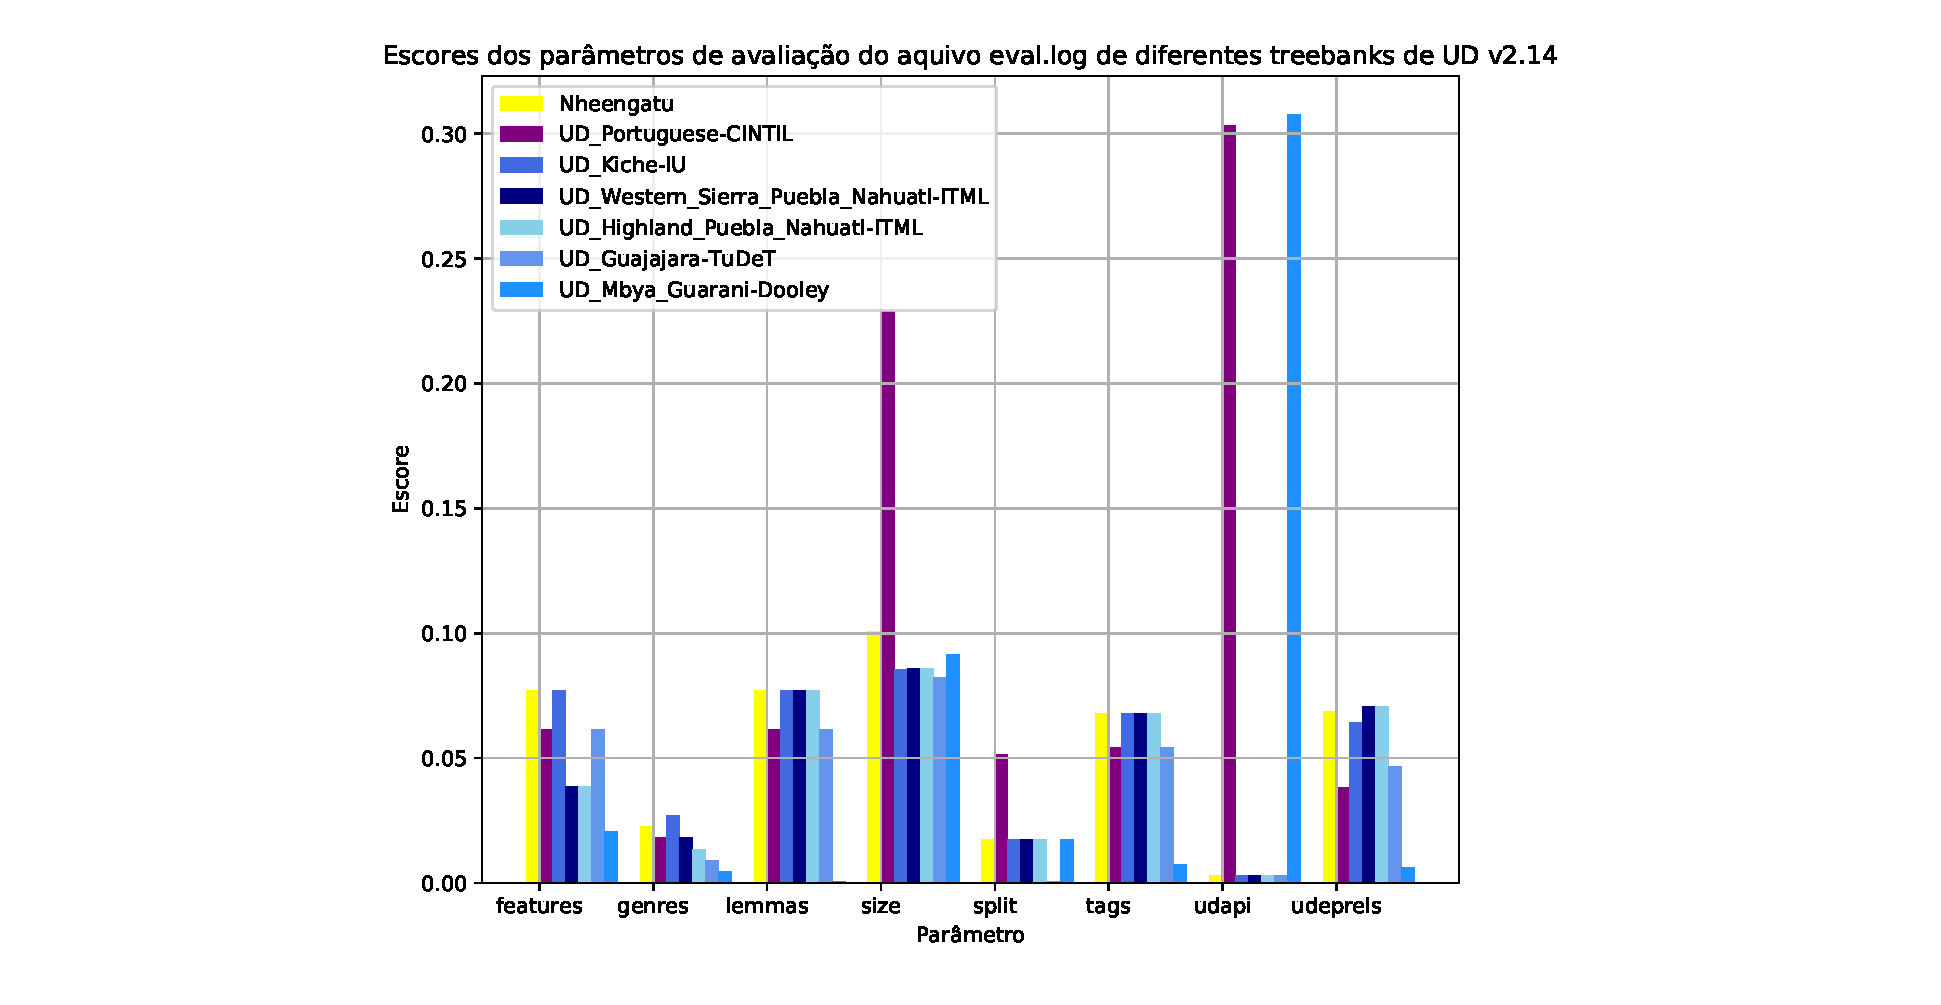
\includegraphics[width=\linewidth]{figures/eval-log.pdf}
    \caption{Avaliação de cinco \tbs~de UD v2.4 em termos de tamanho, diversidade de gêneros textuais, quantidade de erros computados pelo Udapi e diferentes aspectos da anotação.}
    \label{fig:eval-scores}
    \source{Elaboração própria com base nos dados de \textcite{zeman2024universal}.}
  \end{minipage}
\end{figure}

\begin{figure}[htbp]
  \centering
  \begin{minipage}{.75\textwidth}
    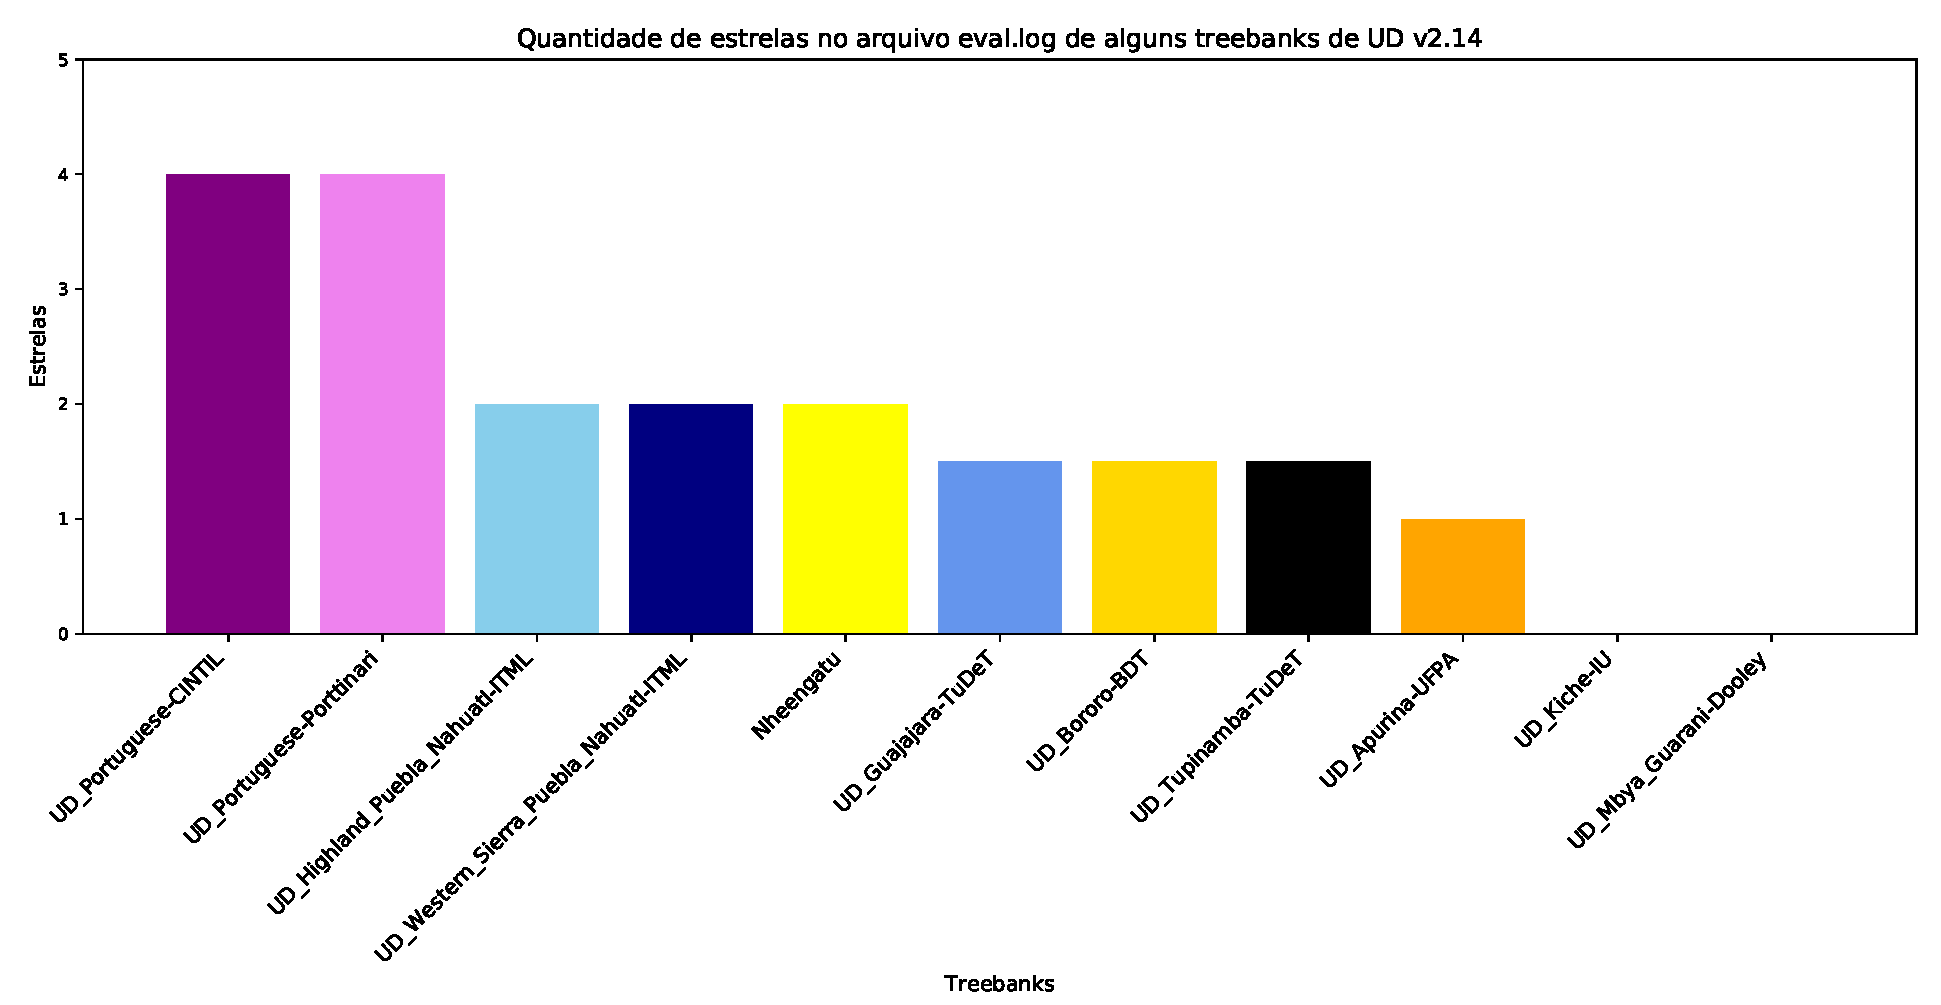
\includegraphics[width=\linewidth]{figures/EvalStarsTBs.pdf}
    \caption{Quantidade de estrelas de onze \tbs~com base nos escores da Figura \ref{fig:eval-scores}.}
    \label{fig:eval-stars}
    \source{Elaboração própria com base nos dados de \textcite{zeman2024universal}.}
  \end{minipage}
\end{figure}

\section{Considerações finais}\label{sec:finais}
Neste trabalho, partimos da premissa de que a inclusão digital é um fator de sobrevivência das línguas minoritárias. Isso é especialmente relevante no caso do nheengatu, dado o seu papel histórico de língua de contato. Como parte significativa dos falantes utiliza cotidianamente o português, com um índice de 0,97 de suporte digital uma das línguas mais privilegiadas do mundo, o nheengatu, com apenas 0,07, enfrenta mais um cenário adverso após mais de 150 anos de progressivo declínio.

Como aporte ao fortalecimento do nheengatu na seara tecnológica, construímos o \tbc, que reúne sentenças tanto mais curtas quanto mais longas extraídas de um total de 20 publicações de diferentes gêneros e épocas. Com 1,28 a 1,64 vezes mais palavras e 1,02 a 1,62 mais sentenças que os outros cinco maiores \tbs~de línguas ameríndias na versão v2.14 da \udc, o \tbc~iguala ou supera estes na maioria das dimensões aferidas pelo \textit{script} \href{https://github.com/UniversalDependencies/tools/blob/master/conllu-stats.pl}{conllu-stats.pl}, notadamente no que tange aos traços morfológicos, integrando o grupo de \tbs~de línguas ameríndias com a maior quantidade de estrelas. Todas essas características parecem propícias ao treino de um \textit{parser} voltado para anotação das demais sentenças do mesmo conjunto de publicações de onde provêm as sentenças atuais do \tb.    

Apesar de todos esses avanços, ainda há um longo caminho a percorrer para alcançar um \textit{parser} do nheengatu com desempenho próximo ao índice LAS de 95\% que \textcite{lopes-pardo-2024-towards-k} obtiveram no \textit{parsing} do português a partir de um \tb~de 8.418 sentenças. Para tanto, precisaríamos pelo menos quintuplicar o tamanho atual do \tbc, abarcando uma parcela maior de sentenças das fontes listadas na Figura \ref{fig:freqsources}. Num experimento de \textit{parsing} utilizando o UDPipe 1.2 com a versão anterior do \tb, \vquatro~obteve, por meio do método de décupla validação cruzada, índices de LAS de 64,51\% $\pm$1,85\% e 81,17\% $\pm$1,02\% para texto cru e texto com etiquetas-ouro, respectivamente. Em sentenças desambiguadas com etiquetas do conjunto XPOS e providas de etiquetas especiais prefixadas por \texttt{/=} para tratamento de palavras desconhecidas, num cenário análogo ao \textit{parsing} com etiquetas-ouro, o Yauti obteve LAS de 73,2\% \pvtres, 7,97 pontos percentuais abaixo do modelo do UDPipe. 

Isso sugere integrar um modelo treinado com mais sentenças no fluxograma de anotação da Figura \ref{fig:fluxograma-anotacao}. As Figuras \ref{fig:yauti-stradelli} e \ref{fig:udpipe-stradelli} permitem antecipar as vantagens da utilização do UDPipe: o \textit{parser} resolve automaticamente a ambiguidade da palavra \textit{kwá}, que, no exemplo em questão, funciona como advérbio ao invés de pronome ou determinante. No entanto, a Figura \ref{fig:udpipe-sapupema} evidencia um problema desse \textit{parser} no tratamento de palavras que inexistem no \textit{corpus} de treino e fogem ao padrão morfológico mais geral. De fato, o \textit{parser} não reconheceu o prefixo relacional de contiguidade desse substantivo poliforme, tratando-o como uniforme. Esse tipo de erro poderia passar despercebido a um anotador humano. O Yauti, pelo contrário, ao não gerar análise alguma para palavras desconhecidas, força o anotador a pesquisá-las em \textcite{avila2021}, incluindo-as no léxico da ferramenta, ou empregar as etiquetas especiais. 


\begin{figure}[htbp]
  \centering
  \begin{minipage}{.75\textwidth}
    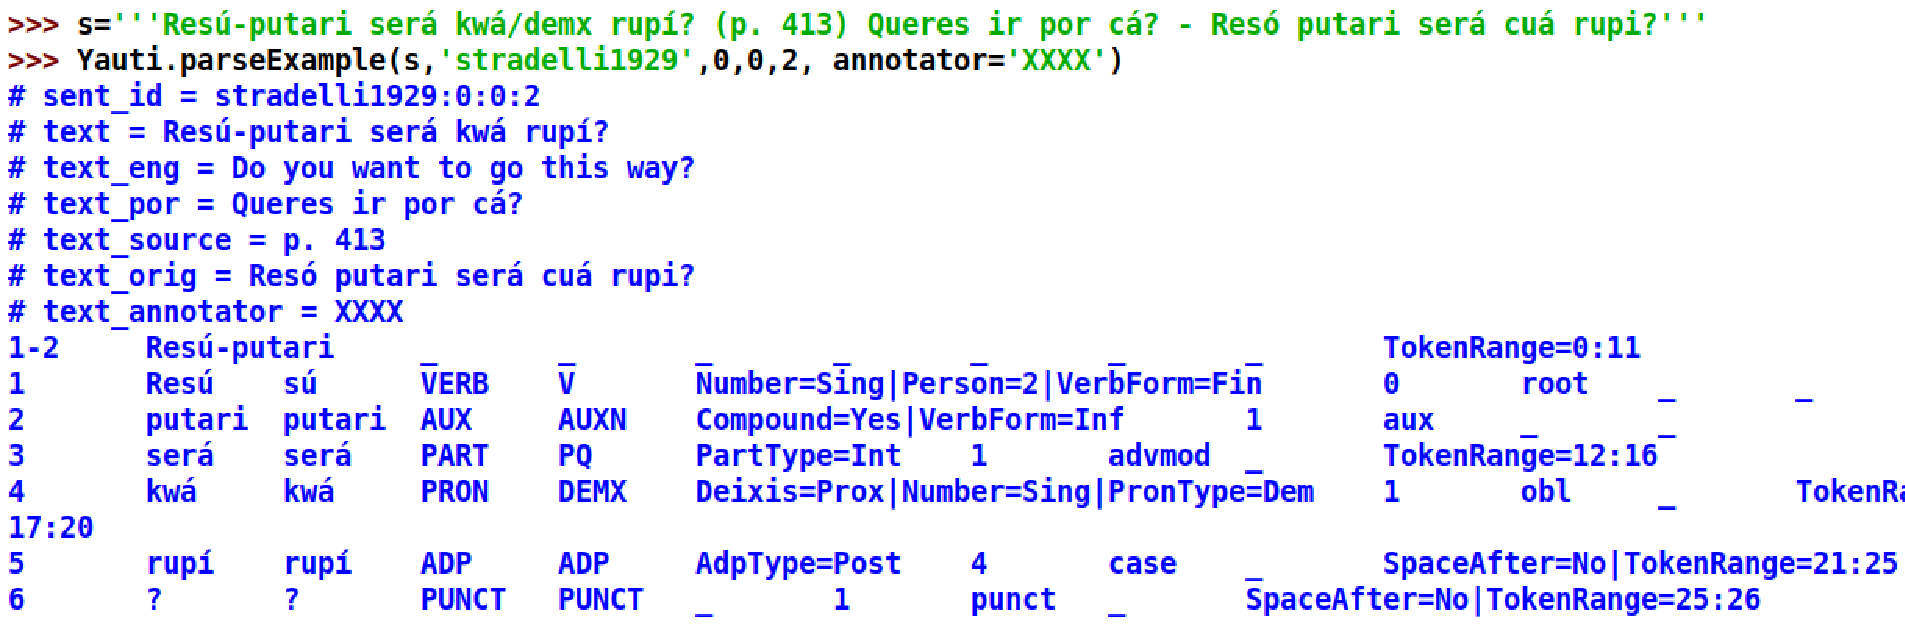
\includegraphics[width=\linewidth]{figures/yauti-stradelli.pdf}
    \caption{Análise de uma nova sentença com o Yauti.}
    \label{fig:yauti-stradelli}
    \source{Elaboração própria.}
  \end{minipage}
\end{figure}

\begin{figure}[htbp]
  \centering
  \begin{minipage}{.75\textwidth}
    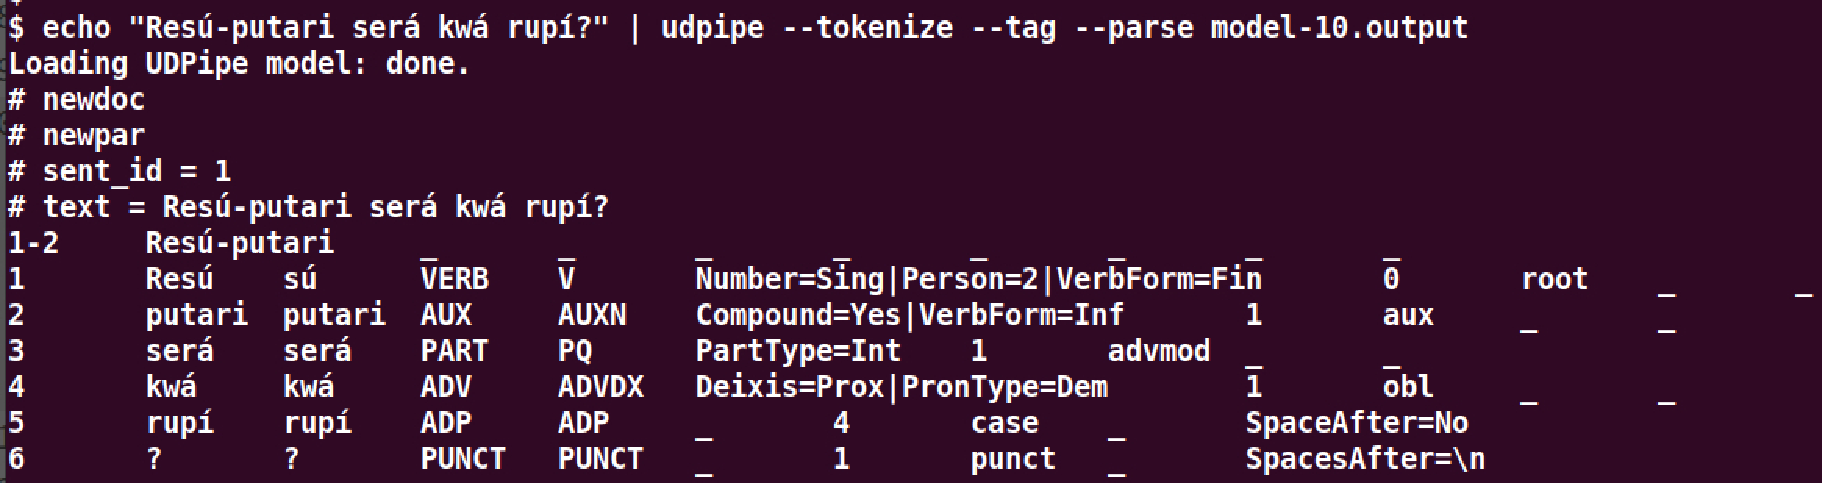
\includegraphics[width=\linewidth]{figures/udpipe-stradelli.pdf}
    \caption{Análise da sentença da Figura \ref{fig:yauti-stradelli} com um dos modelos do UDPipe 1.2. utilizados no experimento de décupla validação cruzada de \vquatro.}
    \label{fig:udpipe-stradelli}
    \source{Elaboração própria.}
  \end{minipage}
\end{figure}

\begin{figure}[htbp]
  \centering
  \begin{minipage}{.75\textwidth}
    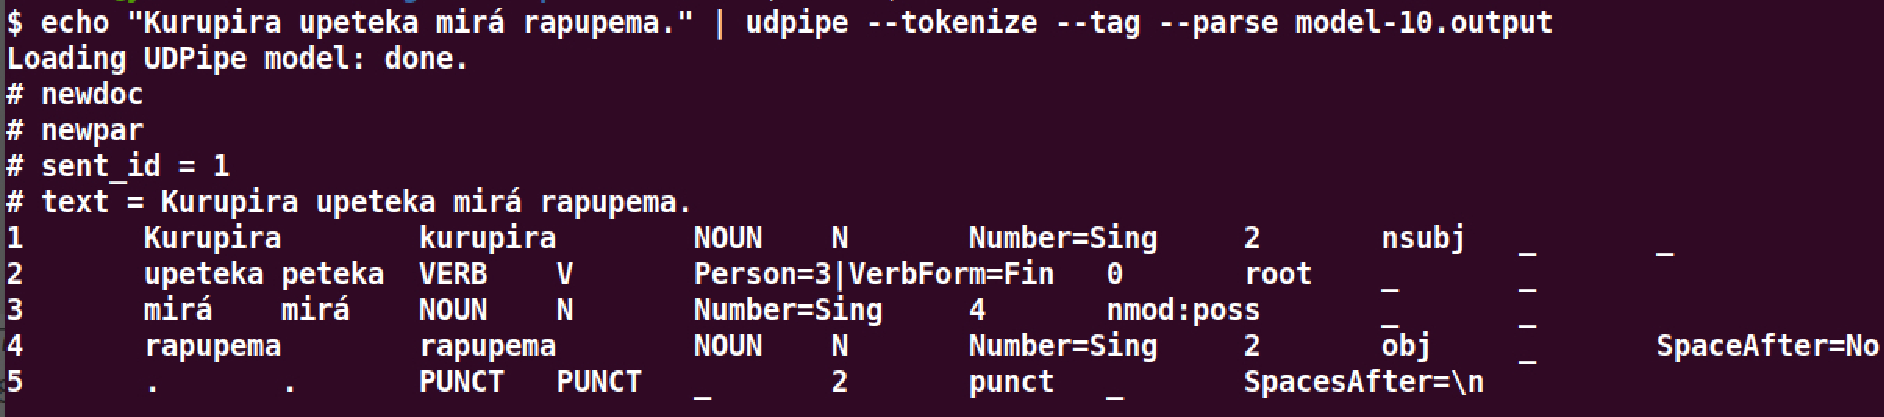
\includegraphics[width=\linewidth]{figures/udpipe-rapupema.pdf}
    \caption{Análise do exemplo da Figura \ref{fig:unknown-word-idle}.}
    \label{fig:udpipe-sapupema}
    \source{Elaboração própria.}
   \end{minipage}
\end{figure}

O \tbc~está em constante expansão e revisão. Uma das tarefas mais urgentes é resolver os erros de anotação apontados pelo Udapi. Esperamos também alcançar 2000 sentenças na próxima \textit{release} de UD e dobrar o número de sentenças revisadas.

\section*{Agradecimentos}

Agradecemos às diversas pessoas e instituições que contribuíram para o \tbc. A Fundação de Amparo à Pesquisa do Estado de São Paulo (FAPESP), no âmbito do projeto \href{https://bv.fapesp.br/57063}{DACILAT} (Processo No. 22/09158-5), e a Fundação Cearense de Apoio ao Desenvolvimento Científico e Tecnológico (Funcap) prestaram auxílio financeiro para o engajamento de estudantes na transcrição, anotação e revisão de sentenças. Nesse contexto, destacamos especialmente as contribuições de Juliana Lopes Gurgel, bolsista de treinamento técnico da FAPESP, e Dominick Maia Alexandre, bolsista de iniciação científica da Funcap. Eduardo de Almeida Navarro gentilmente cedeu os materiais textuais de \textcite{navarro2016}. A Editora da Universidade Federal do Amazonas (UFAM), na pessoa do seu diretor, Sérgio Freire, permitiu a utilização dos textos de \textcite{casasnovas2006}. Marcel Twardowsky Avila generosamente compartilhou conosco a sua \textit{expertise} filológica em nheengatu, esclarecendo muitas questões lexicais e gramaticais sobre a língua e adaptando o texto da lenda \textit{Como a noite apareceu} \parencite{magalhaes1876}. João Marcos Cardoso, especialista em pesquisa e curador da \href{https://www.bbm.usp.br/pt-br/}{Biblioteca Brasiliana Guita e José Mindlin} da Universidade de São Paulo (USP), franqueou-nos as transcrições das narrativas de \textcite{Amorim1928} e \textcite{rodrigues1890}, diligentemente realizadas por Gabriela Lourenço Fernandes e Susan Gabriela Huallpa Huanacuni, estagiárias daquela instituição. 

A versão final do artigo beneficiou-se imensamente dos comentários e sugestões dos dois revisores anônimos, a quem somos profundamente gratos. 

Reconhecemos a utilização do ChatGPT para acelerar a escrita de código em Python e \LaTeX. Examinamos, testamos e frequentemente corrigimos cada uma das sugestões dessa ferramenta.

\printbibliography\label{sec:bib}

\end{document}

